\documentclass{book}
\usepackage[a4paper,top=2.5cm,bottom=2.5cm,left=2.5cm,right=2.5cm]{geometry}
\usepackage{makeidx}
\usepackage{natbib}
\usepackage{graphicx}
\usepackage{multicol}
\usepackage{float}
\usepackage{listings}
\usepackage{color}
\usepackage{ifthen}
\usepackage[table]{xcolor}
\usepackage{textcomp}
\usepackage{alltt}
\usepackage{ifpdf}
\ifpdf
\usepackage[pdftex,
            pagebackref=true,
            colorlinks=true,
            linkcolor=blue,
            unicode
           ]{hyperref}
\else
\usepackage[ps2pdf,
            pagebackref=true,
            colorlinks=true,
            linkcolor=blue,
            unicode
           ]{hyperref}
\usepackage{pspicture}
\fi
\usepackage[utf8]{inputenc}
\usepackage{mathptmx}
\usepackage[scaled=.90]{helvet}
\usepackage{courier}
\usepackage{sectsty}
\usepackage{amssymb}
\usepackage[titles]{tocloft}
\usepackage{doxygen}
\lstset{language=C++,inputencoding=utf8,basicstyle=\footnotesize,breaklines=true,breakatwhitespace=true,tabsize=4,numbers=left }
\makeindex
\setcounter{tocdepth}{3}
\renewcommand{\footrulewidth}{0.4pt}
\renewcommand{\familydefault}{\sfdefault}
\hfuzz=15pt
\setlength{\emergencystretch}{15pt}
\hbadness=750
\tolerance=750
\begin{document}
\hypersetup{pageanchor=false,citecolor=blue}
\begin{titlepage}
\vspace*{7cm}
\begin{center}
{\Large My Project }\\
\vspace*{1cm}
{\large Generated by Doxygen 1.8.3.1}\\
\vspace*{0.5cm}
{\small Tue Dec 3 2013 02:22:03}\\
\end{center}
\end{titlepage}
\clearemptydoublepage
\pagenumbering{roman}
\tableofcontents
\clearemptydoublepage
\pagenumbering{arabic}
\hypersetup{pageanchor=true,citecolor=blue}
\chapter{Hierarchical Index}
\section{Class Hierarchy}
This inheritance list is sorted roughly, but not completely, alphabetically\-:\begin{DoxyCompactList}
\item \contentsline{section}{Barra\-Estado}{\pageref{classBarraEstado}}{}
\item \contentsline{section}{Box\-Opciones\-Basicas}{\pageref{classBoxOpcionesBasicas}}{}
\item \contentsline{section}{Celda}{\pageref{classCelda}}{}
\item \contentsline{section}{Columna}{\pageref{classColumna}}{}
\item \contentsline{section}{Info}{\pageref{classInfo}}{}
\item \contentsline{section}{Menu}{\pageref{classMenu}}{}
\item \contentsline{section}{Note\-Probabilidades}{\pageref{classNoteProbabilidades}}{}
\item \contentsline{section}{Persistidor}{\pageref{classPersistidor}}{}
\item \contentsline{section}{Probs}{\pageref{classProbs}}{}
\begin{DoxyCompactList}
\item \contentsline{section}{Prob\-Celdas}{\pageref{classProbCeldas}}{}
\item \contentsline{section}{Prob\-Columnas}{\pageref{classProbColumnas}}{}
\end{DoxyCompactList}
\item \contentsline{section}{Tablero}{\pageref{classTablero}}{}
\item Window\begin{DoxyCompactList}
\item \contentsline{section}{Main\-Window}{\pageref{classMainWindow}}{}
\end{DoxyCompactList}
\end{DoxyCompactList}

\chapter{Class Index}
\section{Class List}
Here are the classes, structs, unions and interfaces with brief descriptions\-:\begin{DoxyCompactList}
\item\contentsline{section}{\hyperlink{classBarraEstado}{Barra\-Estado} }{\pageref{classBarraEstado}}{}
\item\contentsline{section}{\hyperlink{classBoxOpcionesBasicas}{Box\-Opciones\-Basicas} }{\pageref{classBoxOpcionesBasicas}}{}
\item\contentsline{section}{\hyperlink{classCelda}{Celda} }{\pageref{classCelda}}{}
\item\contentsline{section}{\hyperlink{classColumna}{Columna} }{\pageref{classColumna}}{}
\item\contentsline{section}{\hyperlink{classInfo}{Info} }{\pageref{classInfo}}{}
\item\contentsline{section}{\hyperlink{classMainWindow}{Main\-Window} }{\pageref{classMainWindow}}{}
\item\contentsline{section}{\hyperlink{classMenu}{Menu} }{\pageref{classMenu}}{}
\item\contentsline{section}{\hyperlink{classNoteProbabilidades}{Note\-Probabilidades} }{\pageref{classNoteProbabilidades}}{}
\item\contentsline{section}{\hyperlink{classPersistidor}{Persistidor} }{\pageref{classPersistidor}}{}
\item\contentsline{section}{\hyperlink{classProbCeldas}{Prob\-Celdas} }{\pageref{classProbCeldas}}{}
\item\contentsline{section}{\hyperlink{classProbColumnas}{Prob\-Columnas} }{\pageref{classProbColumnas}}{}
\item\contentsline{section}{\hyperlink{classProbs}{Probs} }{\pageref{classProbs}}{}
\item\contentsline{section}{\hyperlink{classTablero}{Tablero} }{\pageref{classTablero}}{}
\end{DoxyCompactList}

\chapter{Class Documentation}
\hypertarget{classBar}{\section{Bar Class Reference}
\label{classBar}\index{Bar@{Bar}}
}
Inheritance diagram for Bar\-:\begin{figure}[H]
\begin{center}
\leavevmode
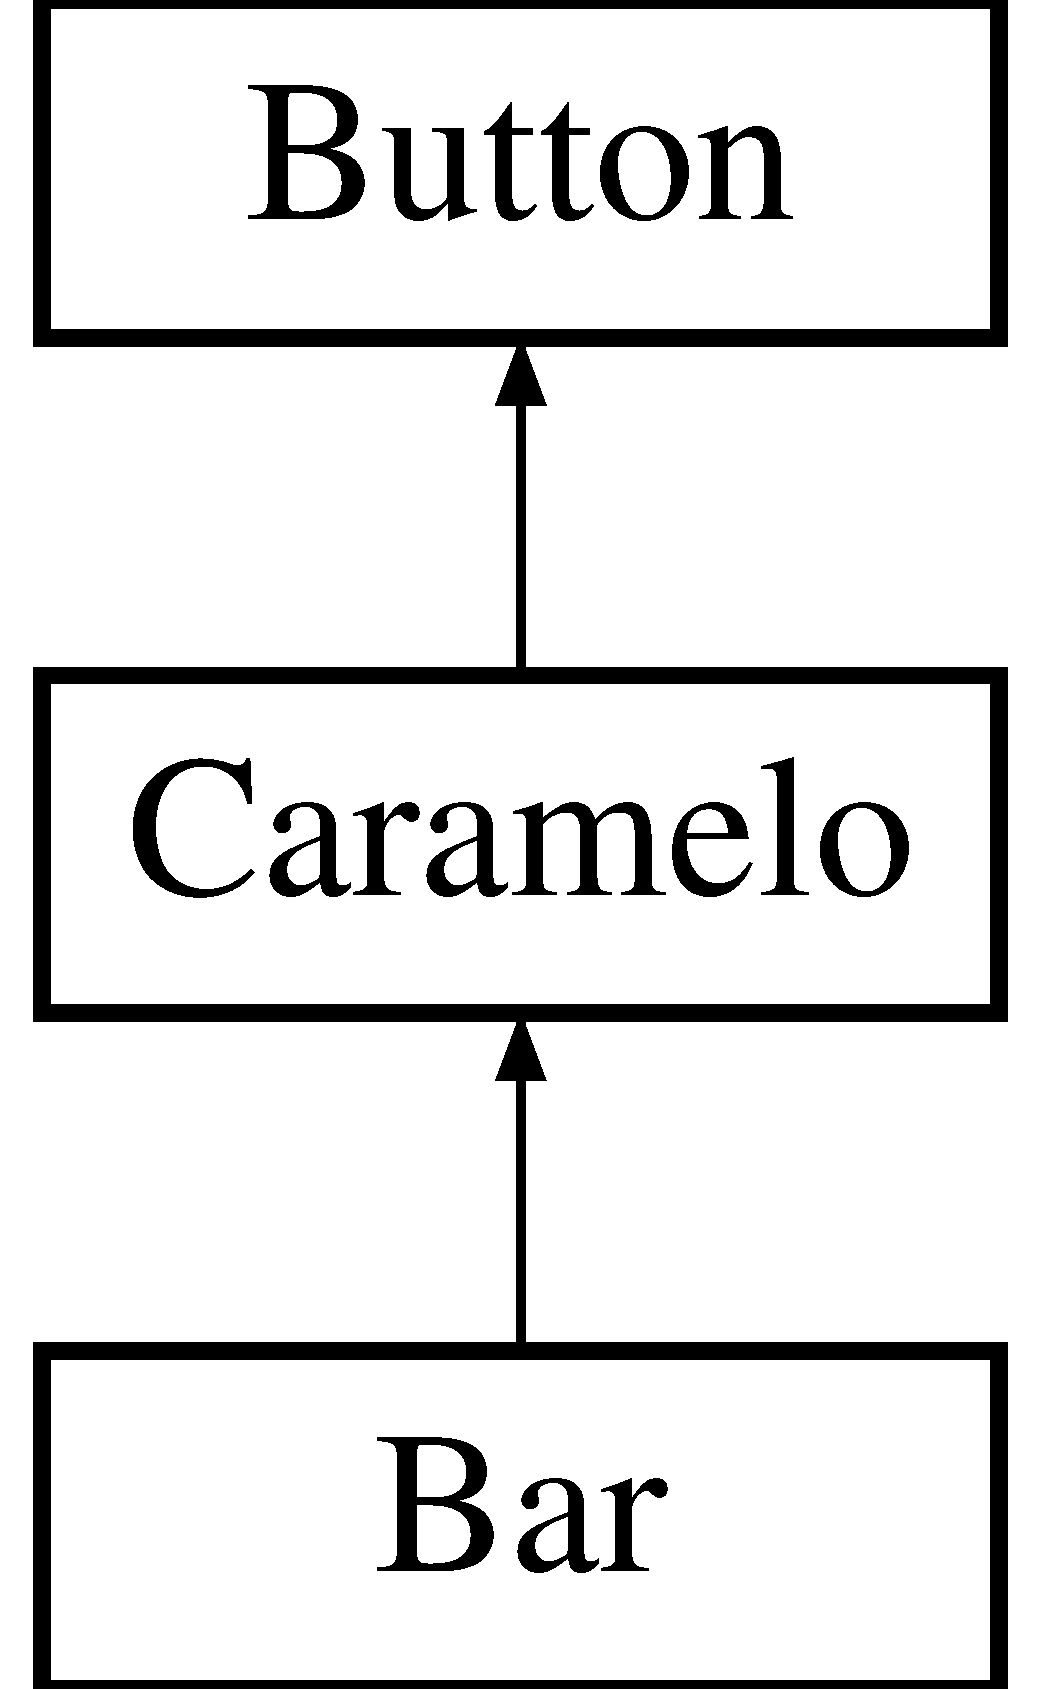
\includegraphics[height=3.000000cm]{classBar}
\end{center}
\end{figure}
\subsection*{Public Member Functions}
\begin{DoxyCompactItemize}
\item 
\hypertarget{classBar_adc31ab40c14d0dbe9f7f41f3bc629598}{{\bfseries Bar} (int id\-Caramelo, bool acostado, const std\-::string \&image\-Name, int i, int j)}\label{classBar_adc31ab40c14d0dbe9f7f41f3bc629598}

\end{DoxyCompactItemize}


The documentation for this class was generated from the following file\-:\begin{DoxyCompactItemize}
\item 
cliente.\-bar.\-h\end{DoxyCompactItemize}

\hypertarget{classButton}{\section{Button Class Reference}
\label{classButton}\index{Button@{Button}}
}
Inheritance diagram for Button\-:\begin{figure}[H]
\begin{center}
\leavevmode
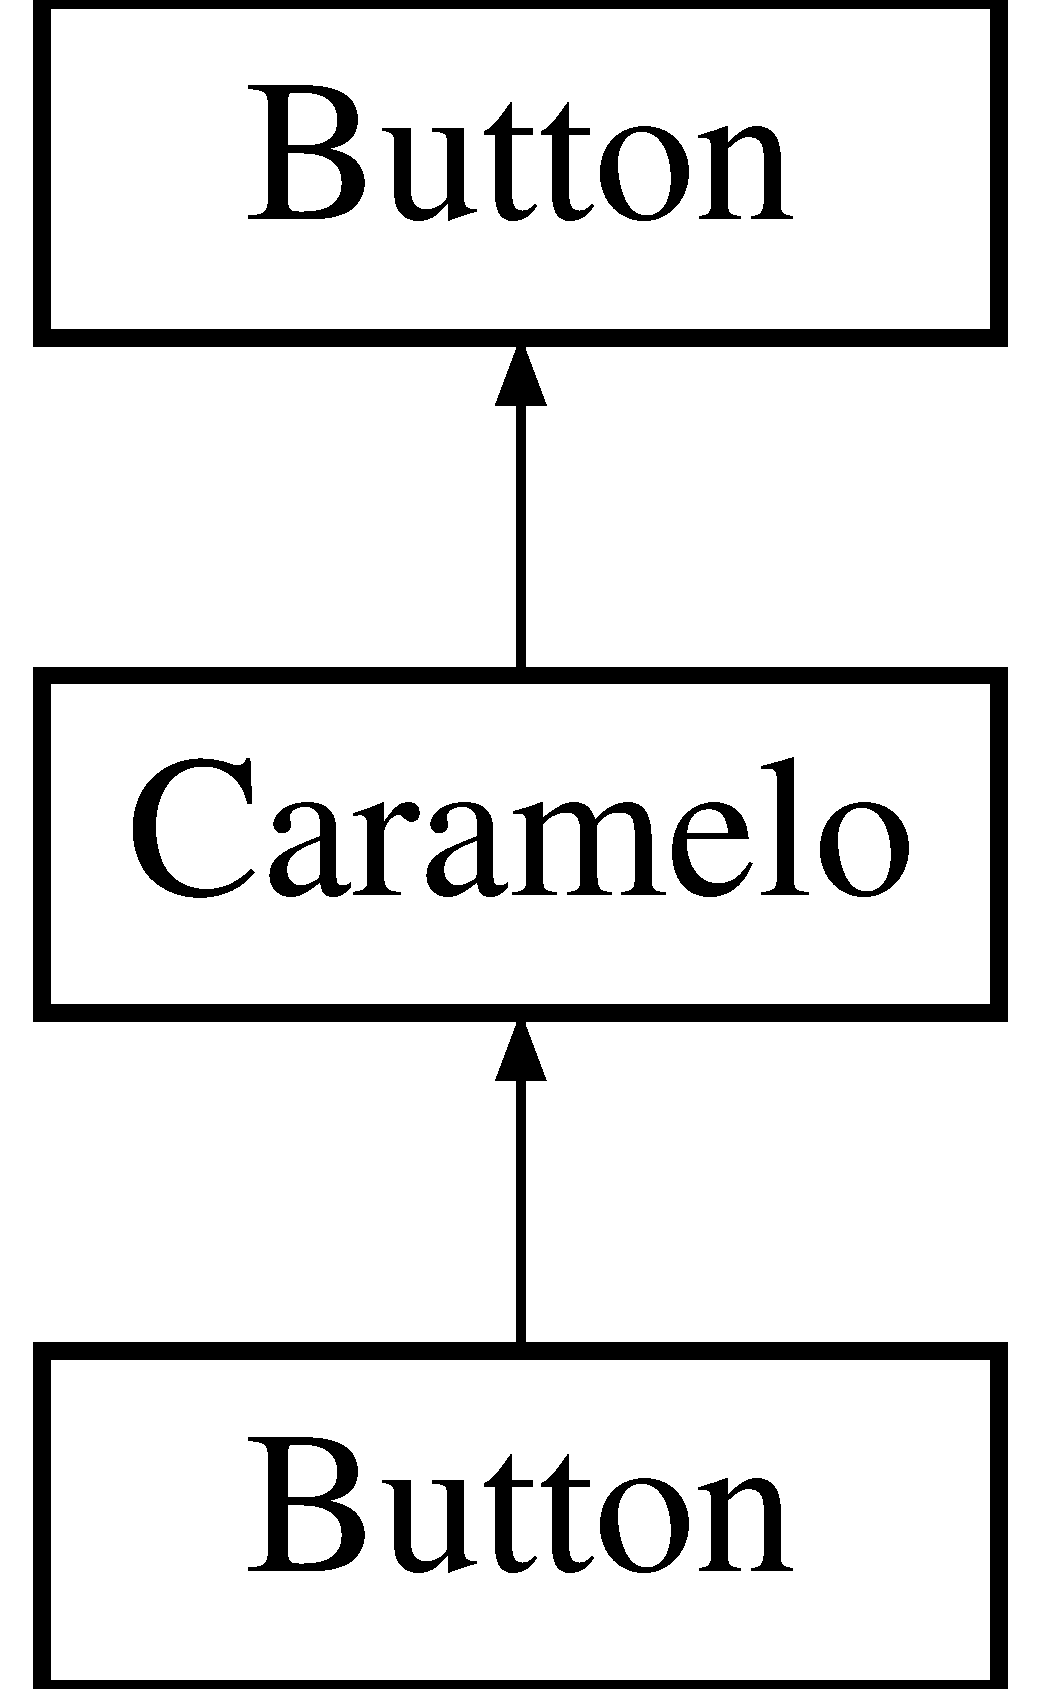
\includegraphics[height=3.000000cm]{classButton}
\end{center}
\end{figure}
\subsection*{Public Member Functions}
\begin{DoxyCompactItemize}
\item 
\hypertarget{classButton_adf73efd6bf6f6bc3c24cf98dc7e79501}{{\bfseries Button} (int id\-Caramelo, const std\-::string \&image\-Name, int i, int j)}\label{classButton_adf73efd6bf6f6bc3c24cf98dc7e79501}

\end{DoxyCompactItemize}


The documentation for this class was generated from the following file\-:\begin{DoxyCompactItemize}
\item 
cliente.\-button.\-h\end{DoxyCompactItemize}

\hypertarget{classCandyFactory}{\section{Candy\-Factory Class Reference}
\label{classCandyFactory}\index{Candy\-Factory@{Candy\-Factory}}
}
\subsection*{Static Public Member Functions}
\begin{DoxyCompactItemize}
\item 
\hypertarget{classCandyFactory_a2dcc29f3fdadc5694c22bcd500f7c4dd}{static \hyperlink{classCaramelo}{Caramelo} $\ast$ {\bfseries crear\-Caramelo} (int id, int i, int j)}\label{classCandyFactory_a2dcc29f3fdadc5694c22bcd500f7c4dd}

\end{DoxyCompactItemize}


The documentation for this class was generated from the following file\-:\begin{DoxyCompactItemize}
\item 
cliente.\-factory\-\_\-caramelos.\-h\end{DoxyCompactItemize}

\hypertarget{classCaramelo}{\section{Caramelo Class Reference}
\label{classCaramelo}\index{Caramelo@{Caramelo}}
}
Inheritance diagram for Caramelo\-:\begin{figure}[H]
\begin{center}
\leavevmode
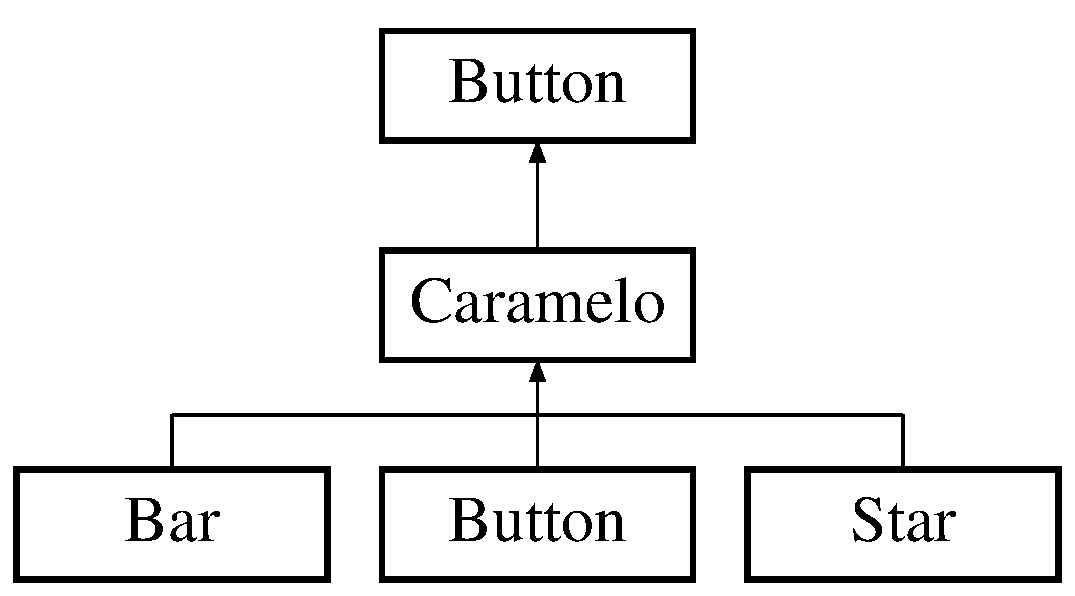
\includegraphics[height=3.000000cm]{classCaramelo}
\end{center}
\end{figure}
\subsection*{Public Member Functions}
\begin{DoxyCompactItemize}
\item 
\hypertarget{classCaramelo_ad644d804aa540a9e1c59c7c8f7f914f3}{{\bfseries Caramelo} (int id\-Caramelo, const std\-::string \&image\-Name, int i, int j)}\label{classCaramelo_ad644d804aa540a9e1c59c7c8f7f914f3}

\item 
bool \hyperlink{classCaramelo_a080a820b554dbeac08583e59151760d4}{mover} (int x, int y)
\item 
\hypertarget{classCaramelo_ae5196c6f1bd18fe6fba0aa15fd91df8d}{bool {\bfseries mover} ()}\label{classCaramelo_ae5196c6f1bd18fe6fba0aa15fd91df8d}

\item 
\hypertarget{classCaramelo_abb98e7f3265f171f4d394898b74e154a}{bool {\bfseries set\-Moviendo} (bool moviendo, int x, int y)}\label{classCaramelo_abb98e7f3265f171f4d394898b74e154a}

\item 
\hypertarget{classCaramelo_accd2373bc4d6ce8cd7837e5a2137e8bb}{bool {\bfseries set\-Moviendo} (bool moviendo)}\label{classCaramelo_accd2373bc4d6ce8cd7837e5a2137e8bb}

\item 
\hypertarget{classCaramelo_af8de0bc3a7f309ad710f19d3a75cbe2e}{void {\bfseries hablar} ()}\label{classCaramelo_af8de0bc3a7f309ad710f19d3a75cbe2e}

\item 
\hypertarget{classCaramelo_ab2c31f222a395e70b878bee9b77d3c74}{int {\bfseries get\-Id} ()}\label{classCaramelo_ab2c31f222a395e70b878bee9b77d3c74}

\item 
\hypertarget{classCaramelo_ac89c8be83cdb7c388d3af32aac6f1f75}{void {\bfseries opacar} ()}\label{classCaramelo_ac89c8be83cdb7c388d3af32aac6f1f75}

\item 
\hypertarget{classCaramelo_ad0f46a451e47d6be971cd3e23afb0eb0}{bool {\bfseries visible} ()}\label{classCaramelo_ad0f46a451e47d6be971cd3e23afb0eb0}

\item 
\hypertarget{classCaramelo_aecb211987104ab0ec6eab44abd8e4f3e}{bool {\bfseries fully\-Visible} ()}\label{classCaramelo_aecb211987104ab0ec6eab44abd8e4f3e}

\item 
\hypertarget{classCaramelo_a49718ac77a61f80481cf7f74c0199df6}{void {\bfseries hacer\-Aparecer} ()}\label{classCaramelo_a49718ac77a61f80481cf7f74c0199df6}

\item 
\hypertarget{classCaramelo_a3e5f9e699d501c9324799e35e4c25394}{int {\bfseries get\-X} ()}\label{classCaramelo_a3e5f9e699d501c9324799e35e4c25394}

\item 
\hypertarget{classCaramelo_a95797573b7a84df706a5e9b5646d67cc}{int {\bfseries get\-X\-Pos} ()}\label{classCaramelo_a95797573b7a84df706a5e9b5646d67cc}

\item 
\hypertarget{classCaramelo_ac6a91c3ecd8f4c483fa11366b6414aba}{int {\bfseries get\-Y} ()}\label{classCaramelo_ac6a91c3ecd8f4c483fa11366b6414aba}

\item 
\hypertarget{classCaramelo_a5942b03955e36c271584d692b90f9cfa}{int {\bfseries get\-Y\-Pos} ()}\label{classCaramelo_a5942b03955e36c271584d692b90f9cfa}

\item 
\hypertarget{classCaramelo_a0e7f0a1c901ea1e90efdab24e58eb96f}{void {\bfseries set\-X} (int x)}\label{classCaramelo_a0e7f0a1c901ea1e90efdab24e58eb96f}

\item 
\hypertarget{classCaramelo_abab0f58f3c11a5e299d0bec578b39890}{void {\bfseries set\-X\-Pos} (int x)}\label{classCaramelo_abab0f58f3c11a5e299d0bec578b39890}

\item 
\hypertarget{classCaramelo_a5ff09d8e6125beb748e2dd188aa4c5f2}{void {\bfseries set\-Y} (int y)}\label{classCaramelo_a5ff09d8e6125beb748e2dd188aa4c5f2}

\item 
\hypertarget{classCaramelo_a936df226e4293c9e77c0f4fe7fee2926}{void {\bfseries set\-Y\-Pos} (int y)}\label{classCaramelo_a936df226e4293c9e77c0f4fe7fee2926}

\end{DoxyCompactItemize}


\subsection{Member Function Documentation}
\hypertarget{classCaramelo_a080a820b554dbeac08583e59151760d4}{\index{Caramelo@{Caramelo}!mover@{mover}}
\index{mover@{mover}!Caramelo@{Caramelo}}
\subsubsection[{mover}]{\setlength{\rightskip}{0pt plus 5cm}bool Caramelo\-::mover (
\begin{DoxyParamCaption}
\item[{int}]{x, }
\item[{int}]{y}
\end{DoxyParamCaption}
)}}\label{classCaramelo_a080a820b554dbeac08583e59151760d4}
Chequea si el caramelo esta en movimiento. Si esta en movimiento, pero se pasan como parametros las coordenadas finales, devolvera false. 
\begin{DoxyParams}{Parameters}
{\em x,\-:} & coordenada final x \\
\hline
{\em y,\-:} & coordeanda final y \\
\hline
\end{DoxyParams}
\begin{DoxyReturn}{Returns}
verdadero si esta en movmiento, falso si no 
\end{DoxyReturn}


The documentation for this class was generated from the following files\-:\begin{DoxyCompactItemize}
\item 
cliente.\-caramelo.\-h\item 
cliente.\-caramelo.\-cpp\end{DoxyCompactItemize}

\hypertarget{classCliente}{\section{Cliente Class Reference}
\label{classCliente}\index{Cliente@{Cliente}}
}


{\ttfamily \#include $<$cliente.\-cliente.\-h$>$}

Inheritance diagram for Cliente\-:\begin{figure}[H]
\begin{center}
\leavevmode
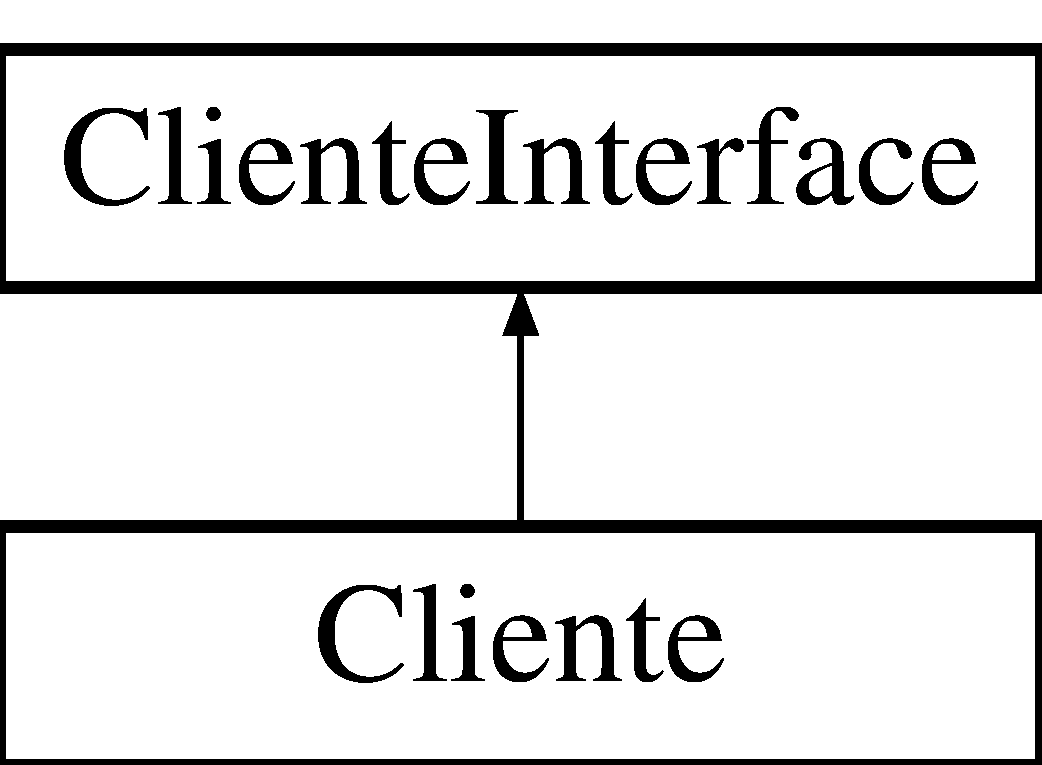
\includegraphics[height=2.000000cm]{classCliente}
\end{center}
\end{figure}
\subsection*{Public Member Functions}
\begin{DoxyCompactItemize}
\item 
void \hyperlink{classCliente_a5b3e7c10e1807cec36a65b527d3dea75}{mostrar\-Ventana\-I\-P} ()
\end{DoxyCompactItemize}


\subsection{Detailed Description}
Clase cliente. Viene a ser la entidad que representa al programa. 

\subsection{Member Function Documentation}
\hypertarget{classCliente_a5b3e7c10e1807cec36a65b527d3dea75}{\index{Cliente@{Cliente}!mostrar\-Ventana\-I\-P@{mostrar\-Ventana\-I\-P}}
\index{mostrar\-Ventana\-I\-P@{mostrar\-Ventana\-I\-P}!Cliente@{Cliente}}
\subsubsection[{mostrar\-Ventana\-I\-P}]{\setlength{\rightskip}{0pt plus 5cm}void Cliente\-::mostrar\-Ventana\-I\-P (
\begin{DoxyParamCaption}
{}
\end{DoxyParamCaption}
)}}\label{classCliente_a5b3e7c10e1807cec36a65b527d3dea75}
Muestra la ventana de Ip y login. 

The documentation for this class was generated from the following files\-:\begin{DoxyCompactItemize}
\item 
cliente.\-cliente.\-h\item 
cliente.\-cliente.\-cpp\end{DoxyCompactItemize}

\hypertarget{classClienteInterface}{\section{Cliente\-Interface Class Reference}
\label{classClienteInterface}\index{Cliente\-Interface@{Cliente\-Interface}}
}


{\ttfamily \#include $<$cliente.\-cliente\-\_\-interface.\-h$>$}

Inheritance diagram for Cliente\-Interface\-:\begin{figure}[H]
\begin{center}
\leavevmode
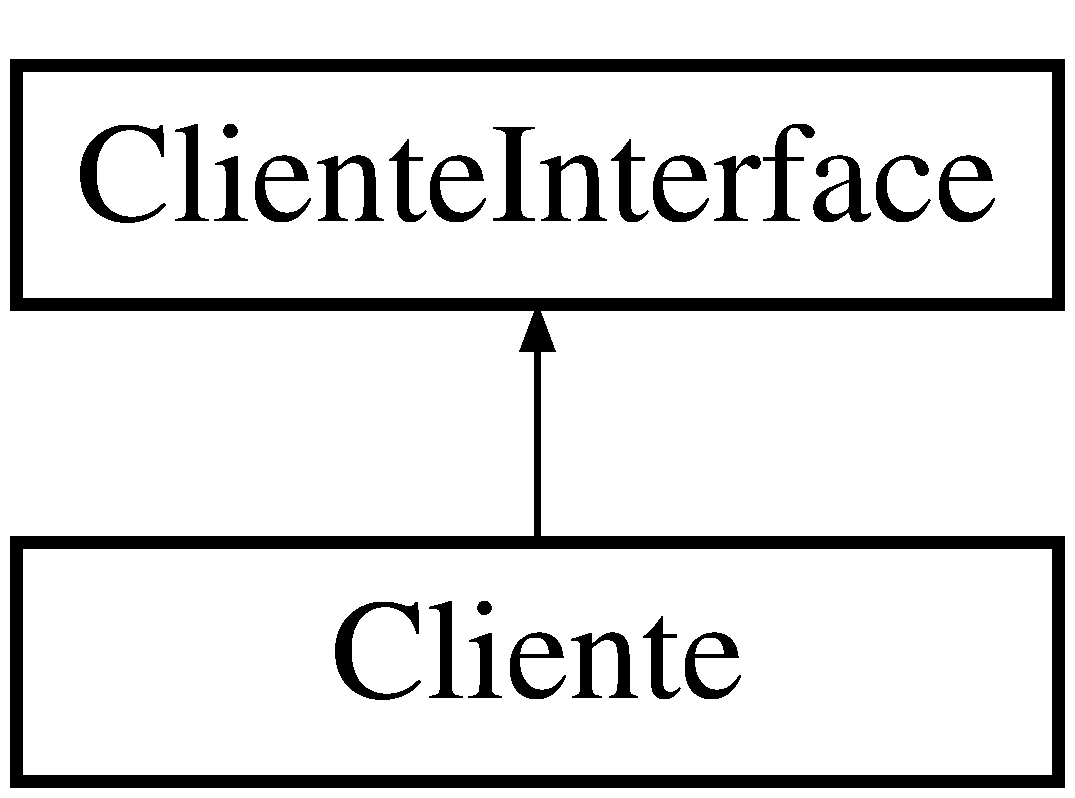
\includegraphics[height=2.000000cm]{classClienteInterface}
\end{center}
\end{figure}
\subsection*{Public Member Functions}
\begin{DoxyCompactItemize}
\item 
virtual void \hyperlink{classClienteInterface_af0e92a73261d0279e7309be763423217}{nuevo\-Mensaje} (Json\-::\-Value \&msj)=0
\end{DoxyCompactItemize}


\subsection{Detailed Description}
Interfaz de cliente. Es usada por \hyperlink{classThreadListener}{Thread\-Listener} para evitar la referencia circular con cliente. 

\subsection{Member Function Documentation}
\hypertarget{classClienteInterface_af0e92a73261d0279e7309be763423217}{\index{Cliente\-Interface@{Cliente\-Interface}!nuevo\-Mensaje@{nuevo\-Mensaje}}
\index{nuevo\-Mensaje@{nuevo\-Mensaje}!ClienteInterface@{Cliente\-Interface}}
\subsubsection[{nuevo\-Mensaje}]{\setlength{\rightskip}{0pt plus 5cm}virtual void Cliente\-Interface\-::nuevo\-Mensaje (
\begin{DoxyParamCaption}
\item[{Json\-::\-Value \&}]{msj}
\end{DoxyParamCaption}
)\hspace{0.3cm}{\ttfamily [pure virtual]}}}\label{classClienteInterface_af0e92a73261d0279e7309be763423217}
Agrega un nuevo mensaje a la cola de mensajes (bloque el mutex de la cola) 

The documentation for this class was generated from the following file\-:\begin{DoxyCompactItemize}
\item 
cliente.\-cliente\-\_\-interface.\-h\end{DoxyCompactItemize}

\hypertarget{classGameWindow}{\section{Game\-Window Class Reference}
\label{classGameWindow}\index{Game\-Window@{Game\-Window}}
}


{\ttfamily \#include $<$cliente.\-game.\-h$>$}

Inheritance diagram for Game\-Window\-:\begin{figure}[H]
\begin{center}
\leavevmode
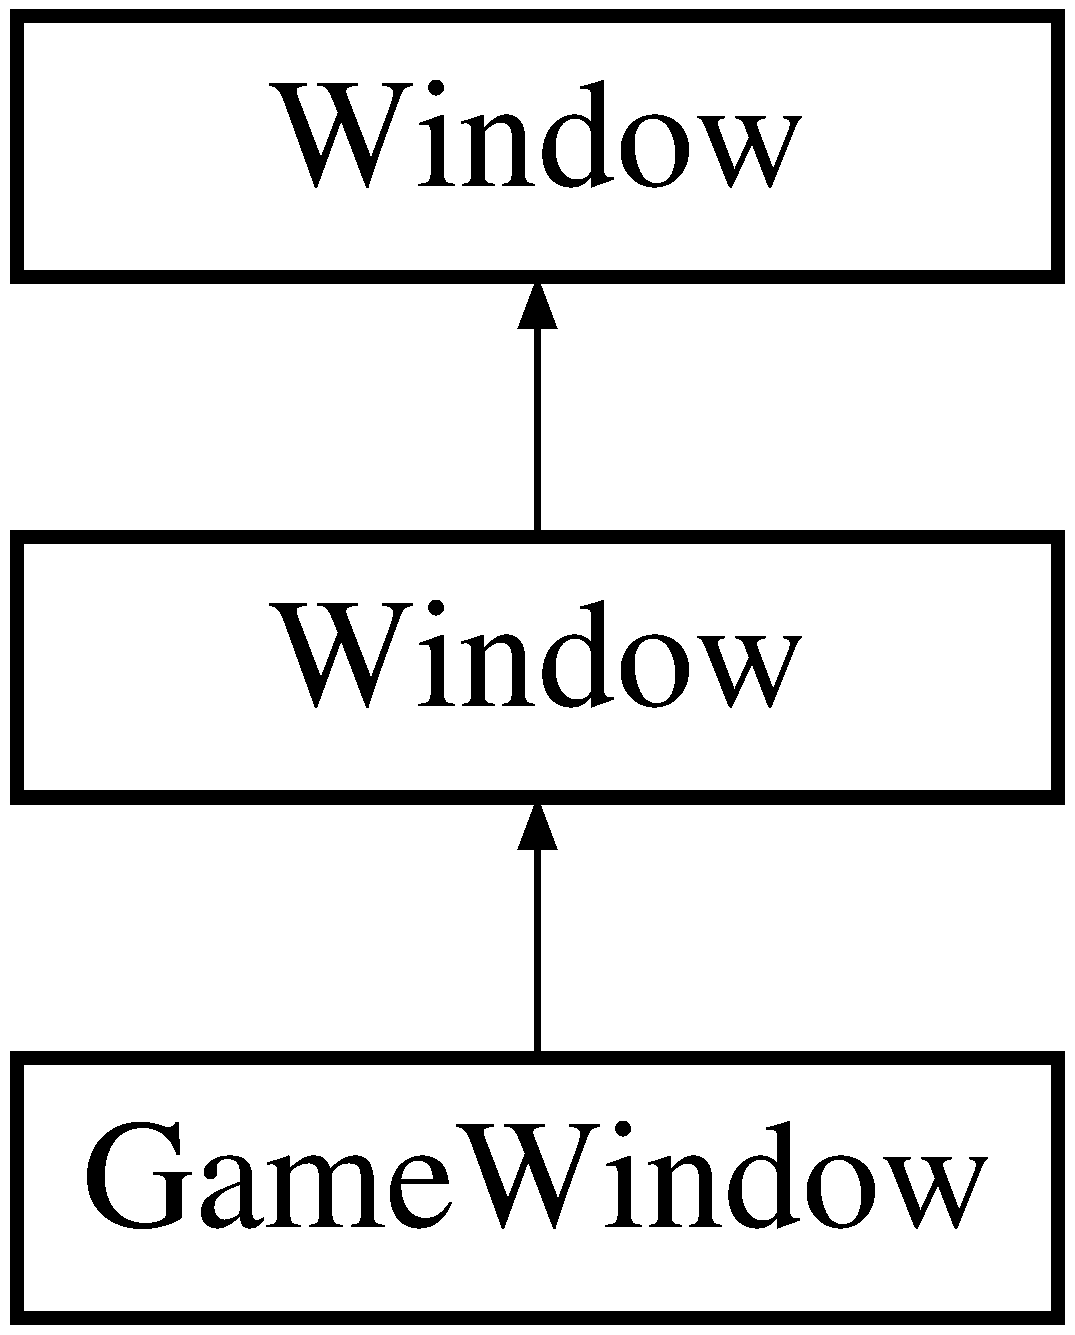
\includegraphics[height=3.000000cm]{classGameWindow}
\end{center}
\end{figure}
\subsection*{Public Member Functions}
\begin{DoxyCompactItemize}
\item 
virtual void \hyperlink{classGameWindow_a3c37318c59913c4232757afebec0e7e1}{mensaje} (Json\-::\-Value \&data)
\end{DoxyCompactItemize}
\subsection*{Protected Member Functions}
\begin{DoxyCompactItemize}
\item 
void \hyperlink{classGameWindow_ae8050c61cfb1a8e92b90e804ae52440f}{on\-\_\-mensaje} ()
\item 
\hypertarget{classGameWindow_ada57617f6a596aae2afabb6af2c4f8c5}{void {\bfseries on\-\_\-start\-\_\-game} ()}\label{classGameWindow_ada57617f6a596aae2afabb6af2c4f8c5}

\item 
\hypertarget{classGameWindow_a88f3f68a6d6b3ee5e9c70f17e7c354bf}{void {\bfseries on\-\_\-salir\-\_\-game} ()}\label{classGameWindow_a88f3f68a6d6b3ee5e9c70f17e7c354bf}

\item 
\hypertarget{classGameWindow_ae7f894b692d4473320e5fb8434a9b087}{void {\bfseries on\-\_\-tablero\-\_\-mensaje} (Json\-::\-Value data)}\label{classGameWindow_ae7f894b692d4473320e5fb8434a9b087}

\item 
\hypertarget{classGameWindow_af5db06b0e85117dff0c191b92693d82b}{void {\bfseries on\-\_\-salir} ()}\label{classGameWindow_af5db06b0e85117dff0c191b92693d82b}

\item 
\hypertarget{classGameWindow_a691183a64a0f14adaf29adb8124d81de}{void {\bfseries on\-\_\-desconectar} ()}\label{classGameWindow_a691183a64a0f14adaf29adb8124d81de}

\item 
\hypertarget{classGameWindow_a172ae0b0b00b7b6555772b9423895541}{virtual bool {\bfseries on\-Close} ()}\label{classGameWindow_a172ae0b0b00b7b6555772b9423895541}

\end{DoxyCompactItemize}
\subsection*{Protected Attributes}
\begin{DoxyCompactItemize}
\item 
\hypertarget{classGameWindow_a0a2cc5e0c631c80db7e93a27df9c2aa0}{Menu\-Bar\-Disconnect {\bfseries menubar}}\label{classGameWindow_a0a2cc5e0c631c80db7e93a27df9c2aa0}

\item 
\hypertarget{classGameWindow_a3caa99f7bcc9224449fd803bf80914e5}{Gtk\-::\-V\-Box {\bfseries m\-\_\-\-V\-Box}}\label{classGameWindow_a3caa99f7bcc9224449fd803bf80914e5}

\item 
\hypertarget{classGameWindow_a22ad7c38de3fa392fea3a61620070cb6}{Gtk\-::\-H\-Box {\bfseries pad\-Box}}\label{classGameWindow_a22ad7c38de3fa392fea3a61620070cb6}

\item 
\hypertarget{classGameWindow_aa42a4efd2b698160715828bb6f475ded}{Gtk\-::\-V\-Box {\bfseries main\-V}}\label{classGameWindow_aa42a4efd2b698160715828bb6f475ded}

\item 
\hypertarget{classGameWindow_aa664f8ee7000541aaa15b0064f88334f}{Gtk\-::\-Scrolled\-Window {\bfseries m\-\_\-\-Scrolled\-Window1}}\label{classGameWindow_aa664f8ee7000541aaa15b0064f88334f}

\item 
\hypertarget{classGameWindow_a9fd4b685bf00fc8b671973f2d034cc14}{Gtk\-::\-Text\-View {\bfseries m\-\_\-\-Text\-View1}}\label{classGameWindow_a9fd4b685bf00fc8b671973f2d034cc14}

\item 
\hypertarget{classGameWindow_abcaa6ff85393398d6333c2e71e840255}{Gtk\-::\-H\-Box {\bfseries m\-\_\-\-H\-Box}}\label{classGameWindow_abcaa6ff85393398d6333c2e71e840255}

\item 
\hypertarget{classGameWindow_ab57509e4b69cb9f7b94df23fa8c5164e}{Gtk\-::\-Entry {\bfseries text\-\_\-input}}\label{classGameWindow_ab57509e4b69cb9f7b94df23fa8c5164e}

\item 
\hypertarget{classGameWindow_afa7b1828170515c768052dd85181f4c3}{Glib\-::\-Ref\-Ptr$<$ Gtk\-::\-Text\-Buffer $>$ {\bfseries m\-\_\-ref\-Text\-Buffer1}}\label{classGameWindow_afa7b1828170515c768052dd85181f4c3}

\item 
\hypertarget{classGameWindow_a9fbf1b39329b4c0d070fde365c39ed07}{Gtk\-::\-Button {\bfseries m\-\_\-button\-\_\-send}}\label{classGameWindow_a9fbf1b39329b4c0d070fde365c39ed07}

\item 
\hypertarget{classGameWindow_ad53b5e021b0f8f6fb81ede5b4bd9666c}{Lista\-Usuarios {\bfseries user\-\_\-list}}\label{classGameWindow_ad53b5e021b0f8f6fb81ede5b4bd9666c}

\item 
\hypertarget{classGameWindow_a5fe5ef93d9549faafefb7a803f233a2a}{Gtk\-::\-H\-Box {\bfseries but\-\_\-hbox}}\label{classGameWindow_a5fe5ef93d9549faafefb7a803f233a2a}

\item 
\hypertarget{classGameWindow_ae280c8f6e002ff97599f2c96db1b1f5c}{Gtk\-::\-Button {\bfseries button\-\_\-start}}\label{classGameWindow_ae280c8f6e002ff97599f2c96db1b1f5c}

\item 
\hypertarget{classGameWindow_aa96a0119cc8b7579f2255ce025238c47}{Gtk\-::\-Button {\bfseries button\-\_\-salir}}\label{classGameWindow_aa96a0119cc8b7579f2255ce025238c47}

\item 
\hypertarget{classGameWindow_a0e7bdd4f6c6ce42d43c6b119b7329f5f}{\hyperlink{classTableroJuego}{Tablero\-Juego} $\ast$ {\bfseries tablero\-Juego}}\label{classGameWindow_a0e7bdd4f6c6ce42d43c6b119b7329f5f}

\end{DoxyCompactItemize}
\subsection*{Additional Inherited Members}


\subsection{Detailed Description}
Ventana de espera antes de que se mande la partida a jugar. Basicamente es un chat 

\subsection{Member Function Documentation}
\hypertarget{classGameWindow_a3c37318c59913c4232757afebec0e7e1}{\index{Game\-Window@{Game\-Window}!mensaje@{mensaje}}
\index{mensaje@{mensaje}!GameWindow@{Game\-Window}}
\subsubsection[{mensaje}]{\setlength{\rightskip}{0pt plus 5cm}void Game\-Window\-::mensaje (
\begin{DoxyParamCaption}
\item[{Json\-::\-Value \&}]{data}
\end{DoxyParamCaption}
)\hspace{0.3cm}{\ttfamily [virtual]}}}\label{classGameWindow_a3c37318c59913c4232757afebec0e7e1}
Metodo que reciben los mensajes del servidor, que deben mostrar. 

Implements \hyperlink{classWindow_a6034ea4f54b6647de07b19ff95fb22ae}{Window}.

\hypertarget{classGameWindow_ae8050c61cfb1a8e92b90e804ae52440f}{\index{Game\-Window@{Game\-Window}!on\-\_\-mensaje@{on\-\_\-mensaje}}
\index{on\-\_\-mensaje@{on\-\_\-mensaje}!GameWindow@{Game\-Window}}
\subsubsection[{on\-\_\-mensaje}]{\setlength{\rightskip}{0pt plus 5cm}void Game\-Window\-::on\-\_\-mensaje (
\begin{DoxyParamCaption}
{}
\end{DoxyParamCaption}
)\hspace{0.3cm}{\ttfamily [protected]}}}\label{classGameWindow_ae8050c61cfb1a8e92b90e804ae52440f}
Signal handler del click en el boton de send 

The documentation for this class was generated from the following files\-:\begin{DoxyCompactItemize}
\item 
cliente.\-game.\-h\item 
cliente.\-game.\-cpp\end{DoxyCompactItemize}

\hypertarget{classIpwindow}{\section{Ipwindow Class Reference}
\label{classIpwindow}\index{Ipwindow@{Ipwindow}}
}


{\ttfamily \#include $<$cliente.\-ipwindow.\-h$>$}

Inheritance diagram for Ipwindow\-:\begin{figure}[H]
\begin{center}
\leavevmode
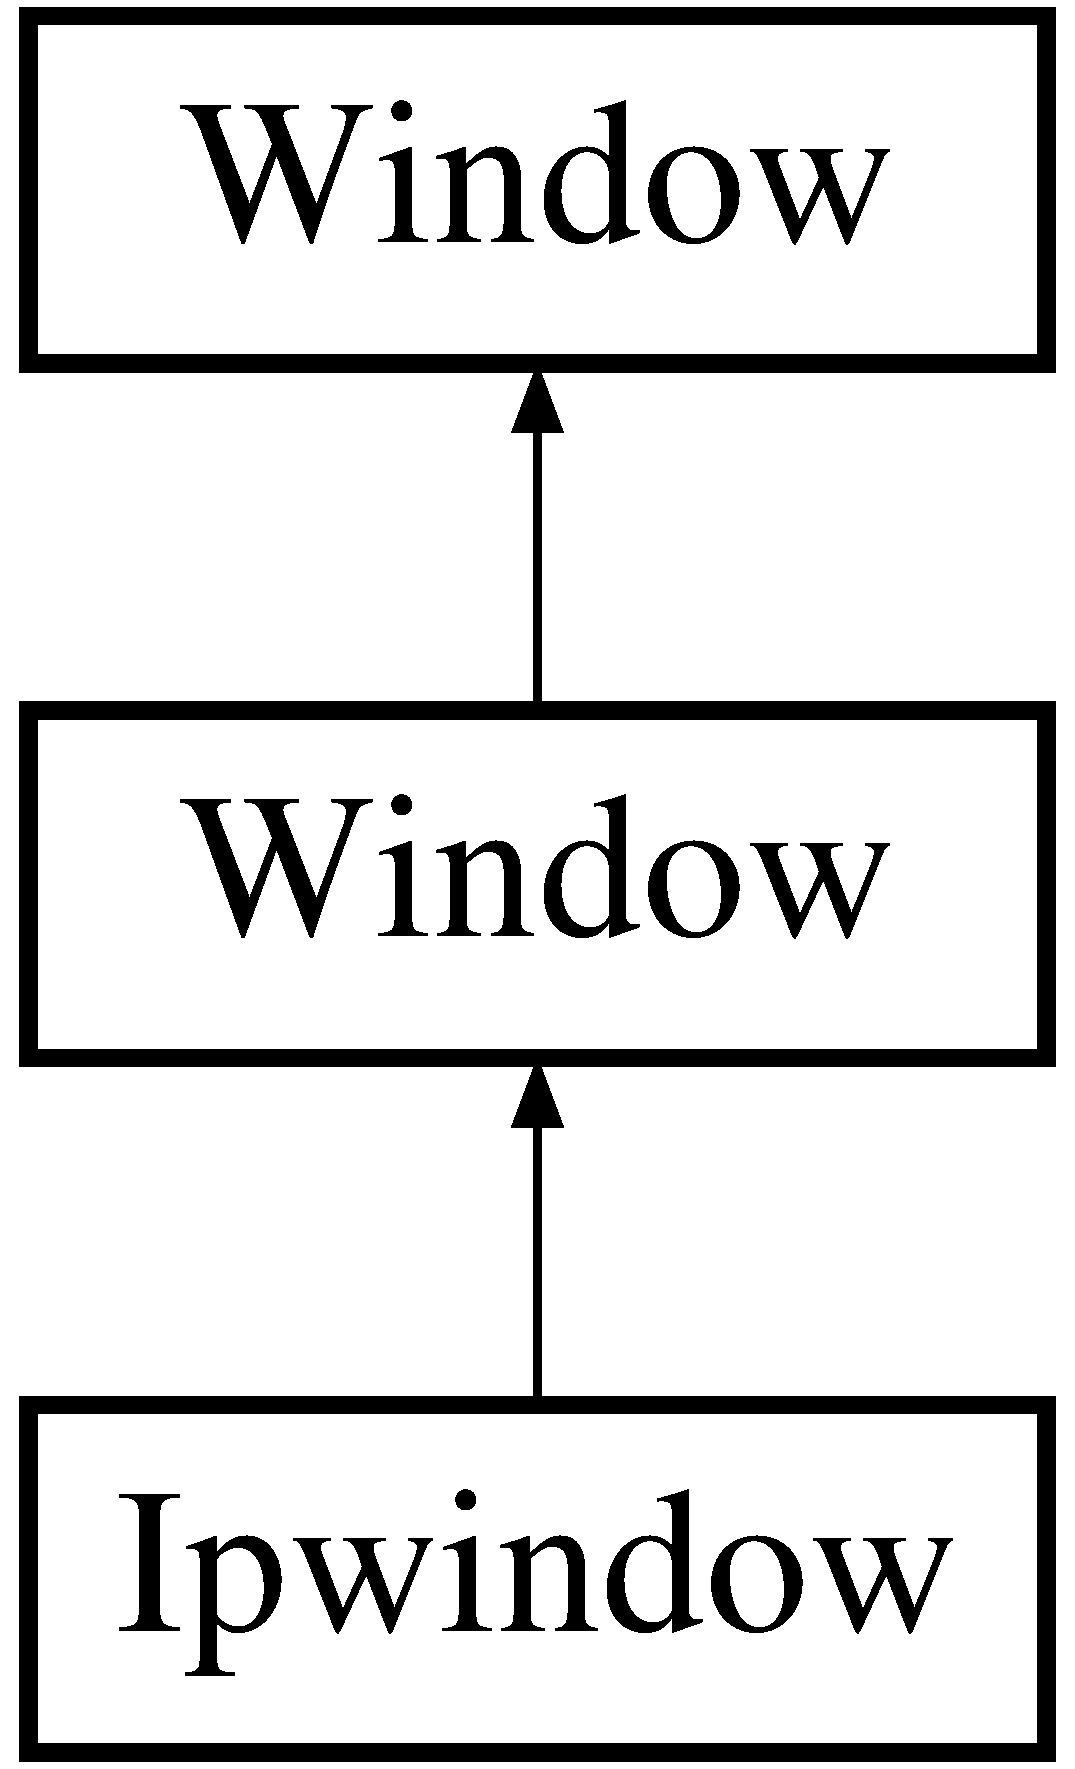
\includegraphics[height=3.000000cm]{classIpwindow}
\end{center}
\end{figure}
\subsection*{Public Types}
\begin{DoxyCompactItemize}
\item 
typedef sigc\-::signal$<$ void, \\*
std\-::string, std\-::string, \\*
std\-::string, bool $>$ \hyperlink{classIpwindow_a44657903a47dd87a70847e74abeb4e68}{type\-\_\-signal\-\_\-conectar}
\end{DoxyCompactItemize}
\subsection*{Public Member Functions}
\begin{DoxyCompactItemize}
\item 
\hypertarget{classIpwindow_a783772352ac8f6dd0cf0a36d57cec35d}{\hyperlink{classIpwindow_a44657903a47dd87a70847e74abeb4e68}{type\-\_\-signal\-\_\-conectar} {\bfseries signal\-\_\-conectar} ()}\label{classIpwindow_a783772352ac8f6dd0cf0a36d57cec35d}

\item 
\hypertarget{classIpwindow_a85d72685748603d08dc6f417288f179d}{void {\bfseries set\-\_\-editable} (bool is\-\_\-editable)}\label{classIpwindow_a85d72685748603d08dc6f417288f179d}

\item 
\hypertarget{classIpwindow_a244eef48968787746981770d1cadb964}{void {\bfseries set\-\_\-text} (std\-::string \&str)}\label{classIpwindow_a244eef48968787746981770d1cadb964}

\item 
virtual void \hyperlink{classIpwindow_ac2c428b415b6a9154ee37de6c8a9dd4d}{mensaje} (Json\-::\-Value \&data)
\end{DoxyCompactItemize}
\subsection*{Protected Member Functions}
\begin{DoxyCompactItemize}
\item 
\hypertarget{classIpwindow_ac8036a10cc5b5f42086291c44a29e7f5}{void {\bfseries on\-\_\-button\-\_\-conectar} ()}\label{classIpwindow_ac8036a10cc5b5f42086291c44a29e7f5}

\item 
\hypertarget{classIpwindow_a8edefd3ac4bdaefeac7bb164e6dba8f1}{virtual bool {\bfseries on\-Close} ()}\label{classIpwindow_a8edefd3ac4bdaefeac7bb164e6dba8f1}

\end{DoxyCompactItemize}
\subsection*{Protected Attributes}
\begin{DoxyCompactItemize}
\item 
\hypertarget{classIpwindow_a28805e1ff41ff9f0b3cffbb30e2bdd0d}{Gtk\-::\-Box {\bfseries m\-\_\-\-H\-Box}}\label{classIpwindow_a28805e1ff41ff9f0b3cffbb30e2bdd0d}

\item 
\hypertarget{classIpwindow_a299006ef69c379869a6a26f471ecedb0}{Gtk\-::\-Box {\bfseries m\-\_\-\-V\-Box}}\label{classIpwindow_a299006ef69c379869a6a26f471ecedb0}

\item 
\hypertarget{classIpwindow_ab8f5709fe4d1ca0afd28544962ad08fd}{Menu\-Bar {\bfseries menubar}}\label{classIpwindow_ab8f5709fe4d1ca0afd28544962ad08fd}

\item 
\hypertarget{classIpwindow_a4a130aa2ef61b6c552bff2f41fc71202}{Gtk\-::\-Image {\bfseries img}}\label{classIpwindow_a4a130aa2ef61b6c552bff2f41fc71202}

\item 
\hypertarget{classIpwindow_af1defcc0555d17fb3c8b0c73c5f9e158}{Label\-Entry {\bfseries m\-\_\-host}}\label{classIpwindow_af1defcc0555d17fb3c8b0c73c5f9e158}

\item 
\hypertarget{classIpwindow_ab1f1531c35d31ae1cba7f57d1cf82ce1}{Label\-Entry {\bfseries m\-\_\-user}}\label{classIpwindow_ab1f1531c35d31ae1cba7f57d1cf82ce1}

\item 
\hypertarget{classIpwindow_a3555431a7095a33d4124818ccc324684}{Label\-Entry {\bfseries m\-\_\-pass}}\label{classIpwindow_a3555431a7095a33d4124818ccc324684}

\item 
\hypertarget{classIpwindow_acea1c6559b084099ca7c44c9687224e1}{Gtk\-::\-Label {\bfseries m\-\_\-text}}\label{classIpwindow_acea1c6559b084099ca7c44c9687224e1}

\item 
\hypertarget{classIpwindow_aa18922eb8ffaffa92abf1abac099a34c}{Gtk\-::\-Check\-Button {\bfseries m\-\_\-check}}\label{classIpwindow_aa18922eb8ffaffa92abf1abac099a34c}

\item 
\hypertarget{classIpwindow_addc90368cfd7161254f0d51e8ccb343a}{Gtk\-::\-H\-Box {\bfseries m\-\_\-\-Button\-\_\-box}}\label{classIpwindow_addc90368cfd7161254f0d51e8ccb343a}

\item 
\hypertarget{classIpwindow_a5284efc19c09dc1a1d5ec4e6011f68ca}{Gtk\-::\-Button {\bfseries m\-\_\-\-Button\-\_\-conectar}}\label{classIpwindow_a5284efc19c09dc1a1d5ec4e6011f68ca}

\item 
\hypertarget{classIpwindow_a6eaceaf031bc400b3347bcfb19f21396}{\hyperlink{classIpwindow_a44657903a47dd87a70847e74abeb4e68}{type\-\_\-signal\-\_\-conectar} {\bfseries m\-\_\-signal\-\_\-conectar}}\label{classIpwindow_a6eaceaf031bc400b3347bcfb19f21396}

\end{DoxyCompactItemize}


\subsection{Detailed Description}
Ventana de login y seleccionar servidor. 

\subsection{Member Typedef Documentation}
\hypertarget{classIpwindow_a44657903a47dd87a70847e74abeb4e68}{\index{Ipwindow@{Ipwindow}!type\-\_\-signal\-\_\-conectar@{type\-\_\-signal\-\_\-conectar}}
\index{type\-\_\-signal\-\_\-conectar@{type\-\_\-signal\-\_\-conectar}!Ipwindow@{Ipwindow}}
\subsubsection[{type\-\_\-signal\-\_\-conectar}]{\setlength{\rightskip}{0pt plus 5cm}typedef sigc\-::signal$<$void, std\-::string, std\-::string, std\-::string, bool$>$ {\bf Ipwindow\-::type\-\_\-signal\-\_\-conectar}}}\label{classIpwindow_a44657903a47dd87a70847e74abeb4e68}
Signal para que el \hyperlink{classCliente}{Cliente} realice la coneccion con el servidor 

\subsection{Member Function Documentation}
\hypertarget{classIpwindow_ac2c428b415b6a9154ee37de6c8a9dd4d}{\index{Ipwindow@{Ipwindow}!mensaje@{mensaje}}
\index{mensaje@{mensaje}!Ipwindow@{Ipwindow}}
\subsubsection[{mensaje}]{\setlength{\rightskip}{0pt plus 5cm}void Ipwindow\-::mensaje (
\begin{DoxyParamCaption}
\item[{Json\-::\-Value \&}]{data}
\end{DoxyParamCaption}
)\hspace{0.3cm}{\ttfamily [virtual]}}}\label{classIpwindow_ac2c428b415b6a9154ee37de6c8a9dd4d}
Metodo que reciben los mensajes del servidor, que deben mostrar. 

Implements \hyperlink{classWindow_a6034ea4f54b6647de07b19ff95fb22ae}{Window}.



The documentation for this class was generated from the following files\-:\begin{DoxyCompactItemize}
\item 
cliente.\-ipwindow.\-h\item 
cliente.\-ipwindow.\-cpp\end{DoxyCompactItemize}

\hypertarget{classListador}{\section{Listador Class Reference}
\label{classListador}\index{Listador@{Listador}}
}


{\ttfamily \#include $<$server.\-listador.\-h$>$}

\subsection*{Static Public Member Functions}
\begin{DoxyCompactItemize}
\item 
static Json\-::\-Value \hyperlink{classListador_aa0ec4ac7afaa1a25676292902bd2ec38}{listar} ()
\item 
\hypertarget{classListador_a202b60bca5249bbfeccd308607d71cc1}{static int {\bfseries get\-Nivel} (std\-::string \&file\-Name)}\label{classListador_a202b60bca5249bbfeccd308607d71cc1}

\item 
\hypertarget{classListador_a5019f12bd56c5dcd3adfae2bb227da5e}{static int {\bfseries get\-Mapa} (std\-::string \&file\-Name, Json\-::\-Value \&mapa)}\label{classListador_a5019f12bd56c5dcd3adfae2bb227da5e}

\end{DoxyCompactItemize}


\subsection{Detailed Description}
Clase que se encarga de proveer metodos para traer informacion acerca de los mapas. 

\subsection{Member Function Documentation}
\hypertarget{classListador_aa0ec4ac7afaa1a25676292902bd2ec38}{\index{Listador@{Listador}!listar@{listar}}
\index{listar@{listar}!Listador@{Listador}}
\subsubsection[{listar}]{\setlength{\rightskip}{0pt plus 5cm}static Json\-::\-Value Listador\-::listar (
\begin{DoxyParamCaption}
{}
\end{DoxyParamCaption}
)\hspace{0.3cm}{\ttfamily [inline]}, {\ttfamily [static]}}}\label{classListador_aa0ec4ac7afaa1a25676292902bd2ec38}
Devuelve un objeto (hash) con\-: \{ nombre de archivo \-: nivel del mapa, \} 

The documentation for this class was generated from the following file\-:\begin{DoxyCompactItemize}
\item 
server.\-listador.\-h\end{DoxyCompactItemize}

\hypertarget{classLogger}{\section{Logger Class Reference}
\label{classLogger}\index{Logger@{Logger}}
}


{\ttfamily \#include $<$common.\-logger.\-h$>$}

\subsection*{Static Public Member Functions}
\begin{DoxyCompactItemize}
\item 
\hypertarget{classLogger_ad9f38f9cc2d75a6207f4972427aa74f1}{static void {\bfseries init} ()}\label{classLogger_ad9f38f9cc2d75a6207f4972427aa74f1}

\item 
\hypertarget{classLogger_a45bbe5b05294541b9ee7e2758c6c30b7}{static void {\bfseries destroy} ()}\label{classLogger_a45bbe5b05294541b9ee7e2758c6c30b7}

\item 
static void \hyperlink{classLogger_aba76d45e4a7eb8704fe408c7e8a0d035}{log} (const std\-::string \&str)
\item 
\hypertarget{classLogger_a5db1668abe71e787c3ad2ad35de6a2e5}{static void {\bfseries log} (const char $\ast$str)}\label{classLogger_a5db1668abe71e787c3ad2ad35de6a2e5}

\end{DoxyCompactItemize}
\subsection*{Protected Member Functions}
\begin{DoxyCompactItemize}
\item 
\hypertarget{classLogger_aae0dca7faca4a0288fa8c379197844e1}{void {\bfseries print} (const std\-::string \&str)}\label{classLogger_aae0dca7faca4a0288fa8c379197844e1}

\end{DoxyCompactItemize}
\subsection*{Protected Attributes}
\begin{DoxyCompactItemize}
\item 
\hypertarget{classLogger_a1cd59b63f5c68f080afe1165730dfbc6}{\hyperlink{classMutex}{Mutex} {\bfseries mut}}\label{classLogger_a1cd59b63f5c68f080afe1165730dfbc6}

\end{DoxyCompactItemize}
\subsection*{Static Protected Attributes}
\begin{DoxyCompactItemize}
\item 
\hypertarget{classLogger_af200e19cfe86c599f8dd1d982f36ee57}{static \hyperlink{classLogger}{Logger} $\ast$ {\bfseries me} = N\-U\-L\-L}\label{classLogger_af200e19cfe86c599f8dd1d982f36ee57}

\end{DoxyCompactItemize}


\subsection{Detailed Description}
Clase singleton usada para logger. Bloque mutex antes de escribir al stdout, se la debe iniciar con init y destruir con destroy. 

\subsection{Member Function Documentation}
\hypertarget{classLogger_aba76d45e4a7eb8704fe408c7e8a0d035}{\index{Logger@{Logger}!log@{log}}
\index{log@{log}!Logger@{Logger}}
\subsubsection[{log}]{\setlength{\rightskip}{0pt plus 5cm}static void Logger\-::log (
\begin{DoxyParamCaption}
\item[{const std\-::string \&}]{str}
\end{DoxyParamCaption}
)\hspace{0.3cm}{\ttfamily [static]}}}\label{classLogger_aba76d45e4a7eb8704fe408c7e8a0d035}
Funciones usadas para logear. 

The documentation for this class was generated from the following files\-:\begin{DoxyCompactItemize}
\item 
common.\-logger.\-h\item 
common.\-logger.\-cpp\end{DoxyCompactItemize}

\hypertarget{classMainWindow}{\section{Main\-Window Class Reference}
\label{classMainWindow}\index{Main\-Window@{Main\-Window}}
}


{\ttfamily \#include $<$cliente.\-main\-\_\-window.\-h$>$}

Inheritance diagram for Main\-Window\-:\begin{figure}[H]
\begin{center}
\leavevmode
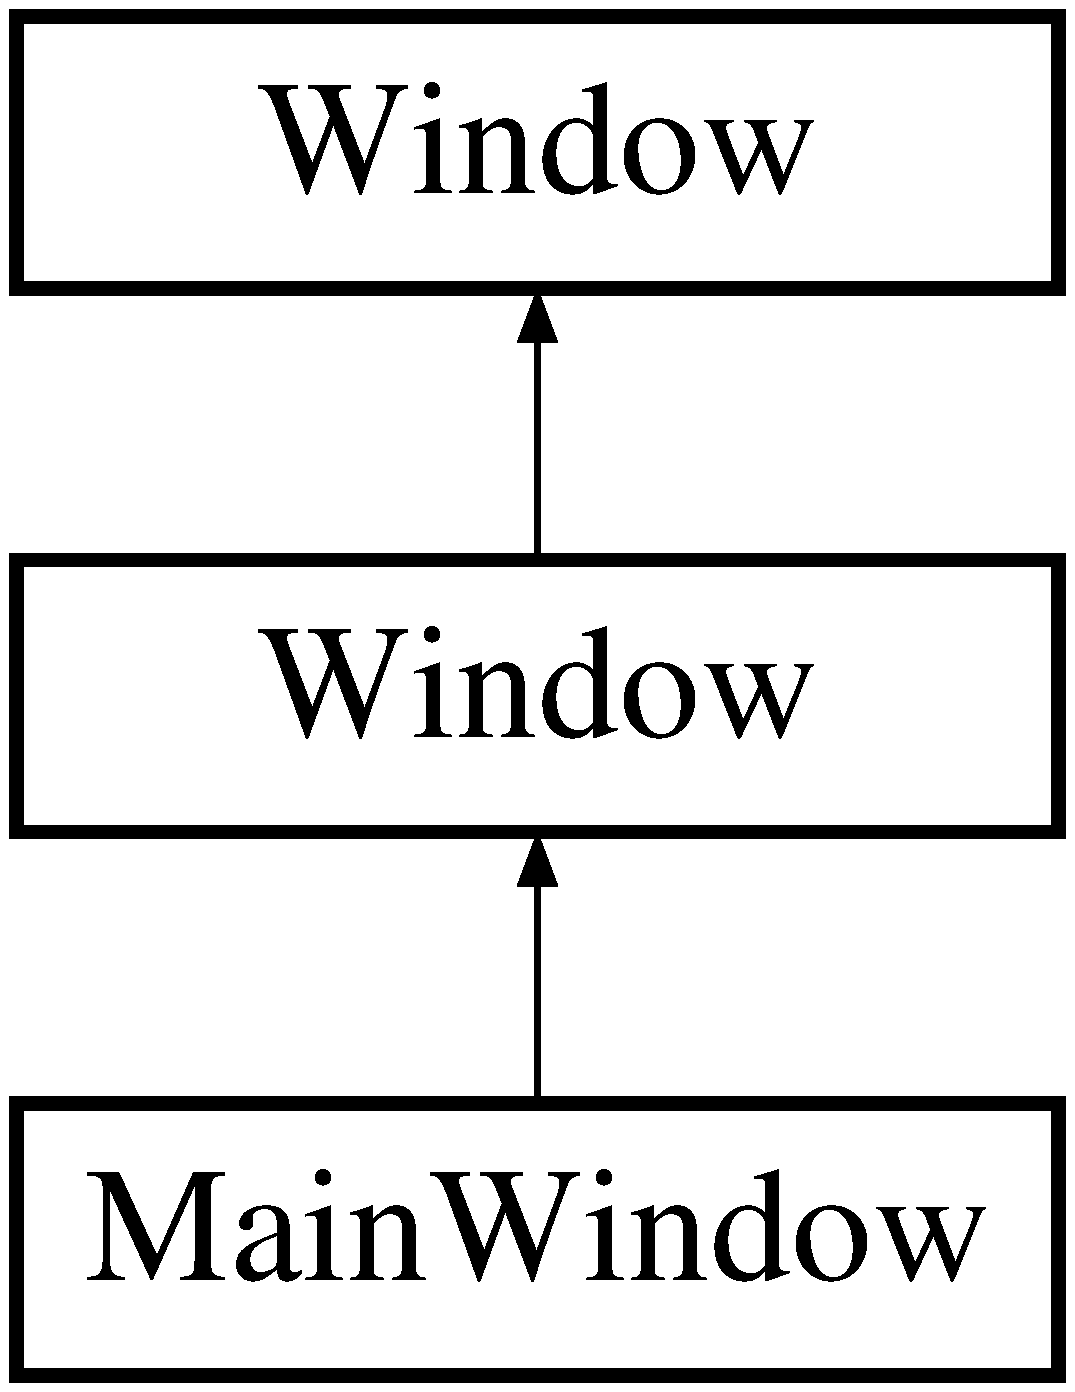
\includegraphics[height=3.000000cm]{classMainWindow}
\end{center}
\end{figure}
\subsection*{Public Member Functions}
\begin{DoxyCompactItemize}
\item 
\hypertarget{classMainWindow_a5a199f2a565bea157bf757965231009b}{void {\bfseries set\-Text} (std\-::string \&str)}\label{classMainWindow_a5a199f2a565bea157bf757965231009b}

\item 
virtual void \hyperlink{classMainWindow_a735c7caa0682694dc016f8bb80ef1f8c}{mensaje} (Json\-::\-Value \&data)
\end{DoxyCompactItemize}
\subsection*{Protected Member Functions}
\begin{DoxyCompactItemize}
\item 
\hypertarget{classMainWindow_a84f1debb16a5d9433115085502664ff1}{void {\bfseries on\-List\-Games} (int code, Json\-::\-Value \&data)}\label{classMainWindow_a84f1debb16a5d9433115085502664ff1}

\item 
\hypertarget{classMainWindow_af1f2f2aa17dcf3f727dca0935e0f9903}{void {\bfseries on\-List\-Maps} (int code, Json\-::\-Value \&data)}\label{classMainWindow_af1f2f2aa17dcf3f727dca0935e0f9903}

\item 
\hypertarget{classMainWindow_a67675f346522095602ef474d1d4a5168}{void {\bfseries on\-\_\-partidas} ()}\label{classMainWindow_a67675f346522095602ef474d1d4a5168}

\item 
\hypertarget{classMainWindow_a9d05b4619e7e5424768cca963922968e}{void {\bfseries join\-\_\-partidas} ()}\label{classMainWindow_a9d05b4619e7e5424768cca963922968e}

\item 
\hypertarget{classMainWindow_a3a1541637c02219b285d5bf9bc6381a1}{void {\bfseries on\-\_\-mapas} ()}\label{classMainWindow_a3a1541637c02219b285d5bf9bc6381a1}

\item 
\hypertarget{classMainWindow_a42724db9575b3be2f1a734351ab51262}{void {\bfseries on\-\_\-crear\-\_\-partida} ()}\label{classMainWindow_a42724db9575b3be2f1a734351ab51262}

\item 
\hypertarget{classMainWindow_acc25dd6bdbfdf9d4cf04c4a099b00e54}{virtual bool {\bfseries on\-Close} ()}\label{classMainWindow_acc25dd6bdbfdf9d4cf04c4a099b00e54}

\end{DoxyCompactItemize}
\subsection*{Protected Attributes}
\begin{DoxyCompactItemize}
\item 
\hypertarget{classMainWindow_adc5c31aa7147c5273128a37c61531935}{Menu\-Bar\-Disconnect {\bfseries menubar}}\label{classMainWindow_adc5c31aa7147c5273128a37c61531935}

\item 
\hypertarget{classMainWindow_a528b74e7fb62a056c7db7e4cc3405f0e}{Gtk\-::\-Notebook {\bfseries tabs}}\label{classMainWindow_a528b74e7fb62a056c7db7e4cc3405f0e}

\item 
\hypertarget{classMainWindow_a3f6985d785f060685e1cd28526fa7f03}{Gtk\-::\-Label {\bfseries label\-Partidas}}\label{classMainWindow_a3f6985d785f060685e1cd28526fa7f03}

\item 
\hypertarget{classMainWindow_a07cf47f1cb3a6fe3e533390db18b9040}{Gtk\-::\-V\-Box {\bfseries m\-\_\-\-V\-Box\-\_\-partidas}}\label{classMainWindow_a07cf47f1cb3a6fe3e533390db18b9040}

\item 
\hypertarget{classMainWindow_ac6f0abacd5af95429201d40b4ec9ca95}{Gtk\-::\-H\-Box {\bfseries m\-\_\-\-H\-Box\-\_\-partidas\-\_\-buttons}}\label{classMainWindow_ac6f0abacd5af95429201d40b4ec9ca95}

\item 
\hypertarget{classMainWindow_ad6a19e7c9f49905bd7bc0c25a1cd50f2}{Gtk\-::\-Button {\bfseries button\-\_\-partidas\-\_\-act}}\label{classMainWindow_ad6a19e7c9f49905bd7bc0c25a1cd50f2}

\item 
\hypertarget{classMainWindow_a1af69f7c49665084fb746433fb7e6fd3}{Gtk\-::\-Button {\bfseries button\-\_\-partidas\-\_\-con}}\label{classMainWindow_a1af69f7c49665084fb746433fb7e6fd3}

\item 
\hypertarget{classMainWindow_a395e40c010bd07252453e9adc64faeb4}{Gtk\-::\-Scrolled\-Window {\bfseries m\-\_\-\-Scrolled\-Partidas}}\label{classMainWindow_a395e40c010bd07252453e9adc64faeb4}

\item 
\hypertarget{classMainWindow_a37807219b285408f8d30efe28a822e62}{Lista\-Partidas {\bfseries m\-\_\-\-Tree\-View}}\label{classMainWindow_a37807219b285408f8d30efe28a822e62}

\item 
\hypertarget{classMainWindow_ae037e61673e84e41a6f28975dd730fd4}{Gtk\-::\-Label {\bfseries label\-Mapas}}\label{classMainWindow_ae037e61673e84e41a6f28975dd730fd4}

\item 
\hypertarget{classMainWindow_a60812cc8e7aa530e73ea1f6515eb7acb}{Gtk\-::\-V\-Box {\bfseries m\-\_\-\-V\-Box\-\_\-mapas}}\label{classMainWindow_a60812cc8e7aa530e73ea1f6515eb7acb}

\item 
\hypertarget{classMainWindow_ab04dad89a39bd6a05ab9b360ca301544}{Gtk\-::\-H\-Box {\bfseries m\-\_\-\-H\-Box\-\_\-mapas\-\_\-buttons}}\label{classMainWindow_ab04dad89a39bd6a05ab9b360ca301544}

\item 
\hypertarget{classMainWindow_ab2355dd68ee5c74d391062fa873ad826}{Gtk\-::\-Button {\bfseries button\-\_\-mapas\-\_\-act}}\label{classMainWindow_ab2355dd68ee5c74d391062fa873ad826}

\item 
\hypertarget{classMainWindow_afc9a680bd1aa98e092db560b592c4467}{Gtk\-::\-Button {\bfseries button\-\_\-mapas\-\_\-cre}}\label{classMainWindow_afc9a680bd1aa98e092db560b592c4467}

\item 
\hypertarget{classMainWindow_a8048011e7fd4242ec20a1a5756ad5bf3}{Gtk\-::\-Scrolled\-Window {\bfseries m\-\_\-\-Scrolled\-Mapas}}\label{classMainWindow_a8048011e7fd4242ec20a1a5756ad5bf3}

\item 
\hypertarget{classMainWindow_a978da20f46529029b3ff46b246fcee09}{Lista\-Mapas {\bfseries m\-\_\-\-Tree\-View\-Mapas}}\label{classMainWindow_a978da20f46529029b3ff46b246fcee09}

\item 
\hypertarget{classMainWindow_a6f9f64b3e9d8baef03dc65513cb68530}{Gtk\-::\-V\-Box {\bfseries main\-V}}\label{classMainWindow_a6f9f64b3e9d8baef03dc65513cb68530}

\item 
\hypertarget{classMainWindow_a7d222c50fa848d67546c7f212875f4c1}{Gtk\-::\-H\-Box {\bfseries tab\-Box}}\label{classMainWindow_a7d222c50fa848d67546c7f212875f4c1}

\item 
\hypertarget{classMainWindow_abe645ed1d8d45e5ba978f324c29d7e09}{Gtk\-::\-Label {\bfseries status\-Label}}\label{classMainWindow_abe645ed1d8d45e5ba978f324c29d7e09}

\end{DoxyCompactItemize}
\subsection*{Additional Inherited Members}


\subsection{Detailed Description}
Ventana de Seleccionar y/o crear partida 

\subsection{Member Function Documentation}
\hypertarget{classMainWindow_a735c7caa0682694dc016f8bb80ef1f8c}{\index{Main\-Window@{Main\-Window}!mensaje@{mensaje}}
\index{mensaje@{mensaje}!MainWindow@{Main\-Window}}
\subsubsection[{mensaje}]{\setlength{\rightskip}{0pt plus 5cm}void Main\-Window\-::mensaje (
\begin{DoxyParamCaption}
\item[{Json\-::\-Value \&}]{data}
\end{DoxyParamCaption}
)\hspace{0.3cm}{\ttfamily [virtual]}}}\label{classMainWindow_a735c7caa0682694dc016f8bb80ef1f8c}
Metodo que reciben los mensajes del servidor, que deben mostrar. 

Implements \hyperlink{classWindow_a6034ea4f54b6647de07b19ff95fb22ae}{Window}.



The documentation for this class was generated from the following files\-:\begin{DoxyCompactItemize}
\item 
cliente.\-main\-\_\-window.\-h\item 
cliente.\-main\-\_\-window.\-cpp\end{DoxyCompactItemize}

\hypertarget{classMutex}{\section{Mutex Class Reference}
\label{classMutex}\index{Mutex@{Mutex}}
}


{\ttfamily \#include $<$common.\-mutex.\-h$>$}

\subsection*{Public Member Functions}
\begin{DoxyCompactItemize}
\item 
int \hyperlink{classMutex_ab779f47fd979c9645703b2110ad48a6b}{lock} ()
\item 
int \hyperlink{classMutex_a73ffa1b2f7fef95563bdb83fed8e57ee}{unlock} ()
\end{DoxyCompactItemize}


\subsection{Detailed Description}
Encapsulamiento del mutex. 

\subsection{Member Function Documentation}
\hypertarget{classMutex_ab779f47fd979c9645703b2110ad48a6b}{\index{Mutex@{Mutex}!lock@{lock}}
\index{lock@{lock}!Mutex@{Mutex}}
\subsubsection[{lock}]{\setlength{\rightskip}{0pt plus 5cm}int Mutex\-::lock (
\begin{DoxyParamCaption}
{}
\end{DoxyParamCaption}
)}}\label{classMutex_ab779f47fd979c9645703b2110ad48a6b}
Lockea al mutex \hypertarget{classMutex_a73ffa1b2f7fef95563bdb83fed8e57ee}{\index{Mutex@{Mutex}!unlock@{unlock}}
\index{unlock@{unlock}!Mutex@{Mutex}}
\subsubsection[{unlock}]{\setlength{\rightskip}{0pt plus 5cm}int Mutex\-::unlock (
\begin{DoxyParamCaption}
{}
\end{DoxyParamCaption}
)}}\label{classMutex_a73ffa1b2f7fef95563bdb83fed8e57ee}
Desloquea al mutex 

The documentation for this class was generated from the following files\-:\begin{DoxyCompactItemize}
\item 
common.\-mutex.\-h\item 
common.\-mutex.\-cpp\end{DoxyCompactItemize}

\hypertarget{classPartida}{\section{Partida Class Reference}
\label{classPartida}\index{Partida@{Partida}}
}


{\ttfamily \#include $<$server.\-partida.\-h$>$}

Inheritance diagram for Partida\-:\begin{figure}[H]
\begin{center}
\leavevmode
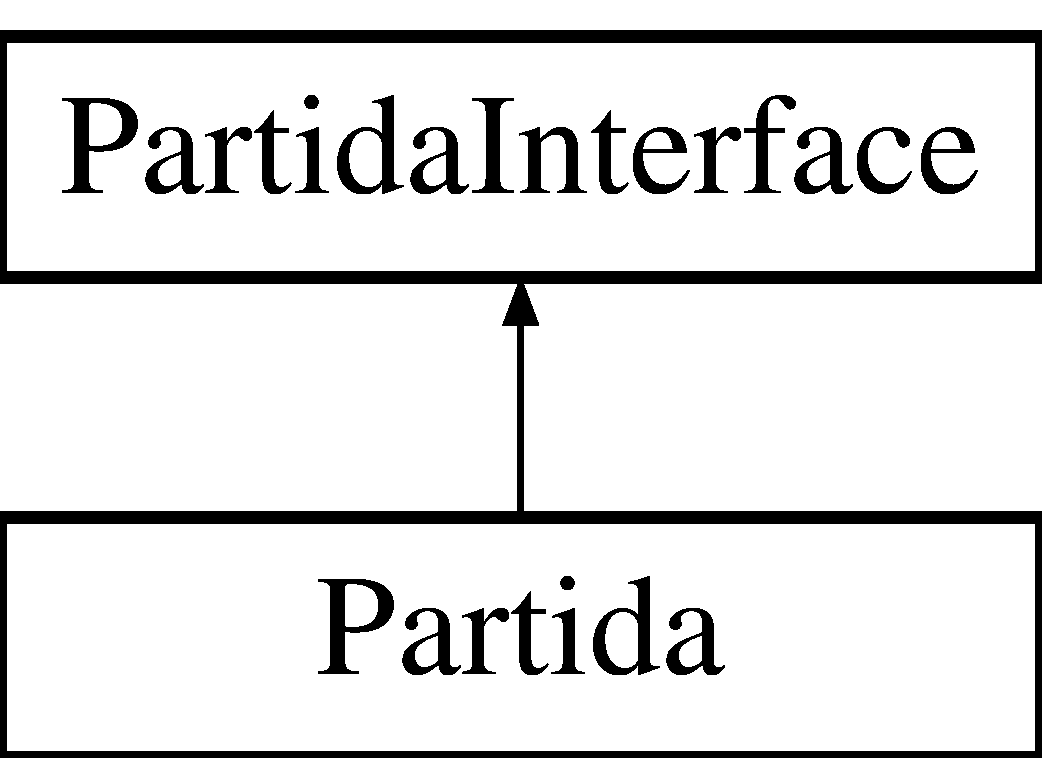
\includegraphics[height=2.000000cm]{classPartida}
\end{center}
\end{figure}
\subsection*{Public Member Functions}
\begin{DoxyCompactItemize}
\item 
\hyperlink{classPartida_a1f7ba9752005060a408c563d8c906767}{Partida} (\hyperlink{classServerInterface}{Server\-Interface} $\ast$server, int nivel, std\-::string \&nombre)
\item 
void \hyperlink{classPartida_a9a6ada8180923f577dbcac9954ef4ac4}{add\-Usuario} (\hyperlink{classThreadSocket}{Thread\-Socket} $\ast$u, Json\-::\-Value \&user)
\item 
void \hyperlink{classPartida_a1676a8787a71098ed0bf65bb27782ceb}{rm\-Usuario} (\hyperlink{classThreadSocket}{Thread\-Socket} $\ast$u)
\item 
int \hyperlink{classPartida_af4035771592061632b5d16879d858cdc}{get\-Nivel} ()
\item 
\hypertarget{classPartida_a8a8fdd55c05f1040dda9fd6df76bfeb2}{int {\bfseries get\-Usuarios} ()}\label{classPartida_a8a8fdd55c05f1040dda9fd6df76bfeb2}

\item 
\hypertarget{classPartida_a32af6c611e9e4556f63633a32c7eb677}{int {\bfseries get\-Max\-Usuarios} ()}\label{classPartida_a32af6c611e9e4556f63633a32c7eb677}

\item 
\hypertarget{classPartida_a74e4a34c63247eb4764a744e54678b8e}{Partida\-Estado {\bfseries get\-Estado} ()}\label{classPartida_a74e4a34c63247eb4764a744e54678b8e}

\item 
\hypertarget{classPartida_a797de83b25e6ff8ebd149f414e9509c7}{std\-::string {\bfseries get\-Nombre} ()}\label{classPartida_a797de83b25e6ff8ebd149f414e9509c7}

\item 
virtual int \hyperlink{classPartida_af5f9e1261116d75042a87ad0b5990700}{mensaje} (Json\-::\-Value \&m, \hyperlink{classThreadSocket}{Thread\-Socket} $\ast$u)
\end{DoxyCompactItemize}
\subsection*{Protected Member Functions}
\begin{DoxyCompactItemize}
\item 
void \hyperlink{classPartida_a515de07436fd6423d7da5d97952031e3}{broadcast\-Msj} (Json\-::\-Value \&msj)
\item 
void \hyperlink{classPartida_a395fb43392e03670c4c6a4a5f23bbd0c}{msj\-Error} (\hyperlink{classThreadSocket}{Thread\-Socket} $\ast$u, const char $\ast$msj)
\item 
\hypertarget{classPartida_af92865c689cd13fc25e16ee0424a6b80}{void {\bfseries msj\-Error} (\hyperlink{classThreadSocket}{Thread\-Socket} $\ast$u, const std\-::string \&msj)}\label{classPartida_af92865c689cd13fc25e16ee0424a6b80}

\end{DoxyCompactItemize}
\subsection*{Protected Attributes}
\begin{DoxyCompactItemize}
\item 
\hypertarget{classPartida_abc3809c4e626bdf312e5b16eb1bd195e}{\hyperlink{classServerInterface}{Server\-Interface} $\ast$ {\bfseries server}}\label{classPartida_abc3809c4e626bdf312e5b16eb1bd195e}

\item 
\hypertarget{classPartida_a462fceca3e2eb8254f06b1d13333a11b}{std\-::vector$<$ \hyperlink{classThreadSocket}{Thread\-Socket} $\ast$ $>$ {\bfseries usuarios}}\label{classPartida_a462fceca3e2eb8254f06b1d13333a11b}

\item 
\hypertarget{classPartida_a3a4835c9999f5eac84192ff85b46d1ad}{std\-::vector$<$ Json\-::\-Value $>$ {\bfseries usuarios\-\_\-data}}\label{classPartida_a3a4835c9999f5eac84192ff85b46d1ad}

\item 
\hypertarget{classPartida_a21aa4e691f8b813a6fb3f79bb7b22a1d}{int {\bfseries nivel}}\label{classPartida_a21aa4e691f8b813a6fb3f79bb7b22a1d}

\item 
\hypertarget{classPartida_a80eb2d37509b6783a1a024c87be409c6}{std\-::string {\bfseries nombre}}\label{classPartida_a80eb2d37509b6783a1a024c87be409c6}

\item 
\hypertarget{classPartida_afb0345f9fa6b54ac3ad4014537dee53d}{\hyperlink{classMutex}{Mutex} {\bfseries usuarios\-Lock}}\label{classPartida_afb0345f9fa6b54ac3ad4014537dee53d}

\item 
\hypertarget{classPartida_a37dc0887b6d2afcbab3373c0dc1f9fcb}{Partida\-Estado {\bfseries estado}}\label{classPartida_a37dc0887b6d2afcbab3373c0dc1f9fcb}

\item 
\hypertarget{classPartida_a514d8e0bcb39b2ae8faae11e3b1ea0e2}{Json\-::\-Value {\bfseries mapa}}\label{classPartida_a514d8e0bcb39b2ae8faae11e3b1ea0e2}

\item 
\hypertarget{classPartida_a0bffb19c265fdc9c973399272719c4d8}{int {\bfseries max\-Usuarios}}\label{classPartida_a0bffb19c265fdc9c973399272719c4d8}

\item 
\hypertarget{classPartida_ac9fac6752ce5e3aa9c8f7ce795911045}{\hyperlink{classMutex}{Mutex} {\bfseries tablero\-Lock}}\label{classPartida_ac9fac6752ce5e3aa9c8f7ce795911045}

\item 
\hypertarget{classPartida_a41e4d9dcd48938f8b52b00a2b136669e}{\hyperlink{classTablero}{Tablero} $\ast$ {\bfseries tablero}}\label{classPartida_a41e4d9dcd48938f8b52b00a2b136669e}

\item 
\hypertarget{classPartida_acbfcc23796a6f67dba56ca8200ee4457}{int {\bfseries puntos\-Max}}\label{classPartida_acbfcc23796a6f67dba56ca8200ee4457}

\end{DoxyCompactItemize}


\subsection{Detailed Description}
Entidad que representa una partida. 

\subsection{Constructor \& Destructor Documentation}
\hypertarget{classPartida_a1f7ba9752005060a408c563d8c906767}{\index{Partida@{Partida}!Partida@{Partida}}
\index{Partida@{Partida}!Partida@{Partida}}
\subsubsection[{Partida}]{\setlength{\rightskip}{0pt plus 5cm}Partida\-::\-Partida (
\begin{DoxyParamCaption}
\item[{{\bf Server\-Interface} $\ast$}]{server, }
\item[{int}]{nivel, }
\item[{std\-::string \&}]{nombre}
\end{DoxyParamCaption}
)}}\label{classPartida_a1f7ba9752005060a408c563d8c906767}
Creador de la partida. 
\begin{DoxyParams}{Parameters}
{\em server\mbox{[}in\mbox{]},\-:} & instancia de servidor \\
\hline
{\em nivel\mbox{[}in\mbox{]},\-:} & nivel de la partida \\
\hline
{\em nombre\mbox{[}in\mbox{]},\-:} & nombre del mapa \\
\hline
\end{DoxyParams}


\subsection{Member Function Documentation}
\hypertarget{classPartida_a9a6ada8180923f577dbcac9954ef4ac4}{\index{Partida@{Partida}!add\-Usuario@{add\-Usuario}}
\index{add\-Usuario@{add\-Usuario}!Partida@{Partida}}
\subsubsection[{add\-Usuario}]{\setlength{\rightskip}{0pt plus 5cm}void Partida\-::add\-Usuario (
\begin{DoxyParamCaption}
\item[{{\bf Thread\-Socket} $\ast$}]{u, }
\item[{Json\-::\-Value \&}]{user}
\end{DoxyParamCaption}
)\hspace{0.3cm}{\ttfamily [virtual]}}}\label{classPartida_a9a6ada8180923f577dbcac9954ef4ac4}
Agrega un usuario a la partida. 
\begin{DoxyParams}{Parameters}
{\em u\mbox{[}in\mbox{]},\-:} & threadsocket del usuario \\
\hline
{\em user\mbox{[}in\mbox{]},\-:} & nombre de usuario \\
\hline
\end{DoxyParams}


Implements \hyperlink{classPartidaInterface}{Partida\-Interface}.

\hypertarget{classPartida_a515de07436fd6423d7da5d97952031e3}{\index{Partida@{Partida}!broadcast\-Msj@{broadcast\-Msj}}
\index{broadcast\-Msj@{broadcast\-Msj}!Partida@{Partida}}
\subsubsection[{broadcast\-Msj}]{\setlength{\rightskip}{0pt plus 5cm}void Partida\-::broadcast\-Msj (
\begin{DoxyParamCaption}
\item[{Json\-::\-Value \&}]{msj}
\end{DoxyParamCaption}
)\hspace{0.3cm}{\ttfamily [protected]}}}\label{classPartida_a515de07436fd6423d7da5d97952031e3}
Envia msj a todos los usuarios de la partida \hypertarget{classPartida_af4035771592061632b5d16879d858cdc}{\index{Partida@{Partida}!get\-Nivel@{get\-Nivel}}
\index{get\-Nivel@{get\-Nivel}!Partida@{Partida}}
\subsubsection[{get\-Nivel}]{\setlength{\rightskip}{0pt plus 5cm}int Partida\-::get\-Nivel (
\begin{DoxyParamCaption}
{}
\end{DoxyParamCaption}
)\hspace{0.3cm}{\ttfamily [virtual]}}}\label{classPartida_af4035771592061632b5d16879d858cdc}
Metodos que devuelven informacion acerca de la partida 

Implements \hyperlink{classPartidaInterface}{Partida\-Interface}.

\hypertarget{classPartida_af5f9e1261116d75042a87ad0b5990700}{\index{Partida@{Partida}!mensaje@{mensaje}}
\index{mensaje@{mensaje}!Partida@{Partida}}
\subsubsection[{mensaje}]{\setlength{\rightskip}{0pt plus 5cm}int Partida\-::mensaje (
\begin{DoxyParamCaption}
\item[{Json\-::\-Value \&}]{m, }
\item[{{\bf Thread\-Socket} $\ast$}]{u}
\end{DoxyParamCaption}
)\hspace{0.3cm}{\ttfamily [virtual]}}}\label{classPartida_af5f9e1261116d75042a87ad0b5990700}
Metodo usado para mandarle mensajes a la partida. 
\begin{DoxyParams}{Parameters}
{\em m\mbox{[}in\mbox{]},\-:} & mensaje encondeado en J\-S\-O\-N que recibe la partida \\
\hline
{\em u\mbox{[}in\mbox{]},\-:} & \hyperlink{classThreadSocket}{Thread\-Socket} que le envio el mensaje \\
\hline
\end{DoxyParams}


Implements \hyperlink{classPartidaInterface_a72c79ab5c06e2ec804260dc98a977e60}{Partida\-Interface}.

\hypertarget{classPartida_a395fb43392e03670c4c6a4a5f23bbd0c}{\index{Partida@{Partida}!msj\-Error@{msj\-Error}}
\index{msj\-Error@{msj\-Error}!Partida@{Partida}}
\subsubsection[{msj\-Error}]{\setlength{\rightskip}{0pt plus 5cm}void Partida\-::msj\-Error (
\begin{DoxyParamCaption}
\item[{{\bf Thread\-Socket} $\ast$}]{u, }
\item[{const char $\ast$}]{msj}
\end{DoxyParamCaption}
)\hspace{0.3cm}{\ttfamily [protected]}}}\label{classPartida_a395fb43392e03670c4c6a4a5f23bbd0c}
Envia un mensaje a u, (E\-V\-E\-N\-T\-\_\-\-G\-A\-M\-E\-\_\-\-M\-S\-G). \hypertarget{classPartida_a1676a8787a71098ed0bf65bb27782ceb}{\index{Partida@{Partida}!rm\-Usuario@{rm\-Usuario}}
\index{rm\-Usuario@{rm\-Usuario}!Partida@{Partida}}
\subsubsection[{rm\-Usuario}]{\setlength{\rightskip}{0pt plus 5cm}void Partida\-::rm\-Usuario (
\begin{DoxyParamCaption}
\item[{{\bf Thread\-Socket} $\ast$}]{u}
\end{DoxyParamCaption}
)\hspace{0.3cm}{\ttfamily [virtual]}}}\label{classPartida_a1676a8787a71098ed0bf65bb27782ceb}
Borra un usuario de la partida 
\begin{DoxyParams}{Parameters}
{\em u\mbox{[}in\mbox{]},\-:} & threasocket del usuario \\
\hline
\end{DoxyParams}


Implements \hyperlink{classPartidaInterface}{Partida\-Interface}.



The documentation for this class was generated from the following files\-:\begin{DoxyCompactItemize}
\item 
server.\-partida.\-h\item 
server.\-partida.\-cpp\end{DoxyCompactItemize}

\hypertarget{classPartidaInterface}{\section{Partida\-Interface Class Reference}
\label{classPartidaInterface}\index{Partida\-Interface@{Partida\-Interface}}
}


{\ttfamily \#include $<$server.\-partida\-\_\-interface.\-h$>$}

Inheritance diagram for Partida\-Interface\-:\begin{figure}[H]
\begin{center}
\leavevmode
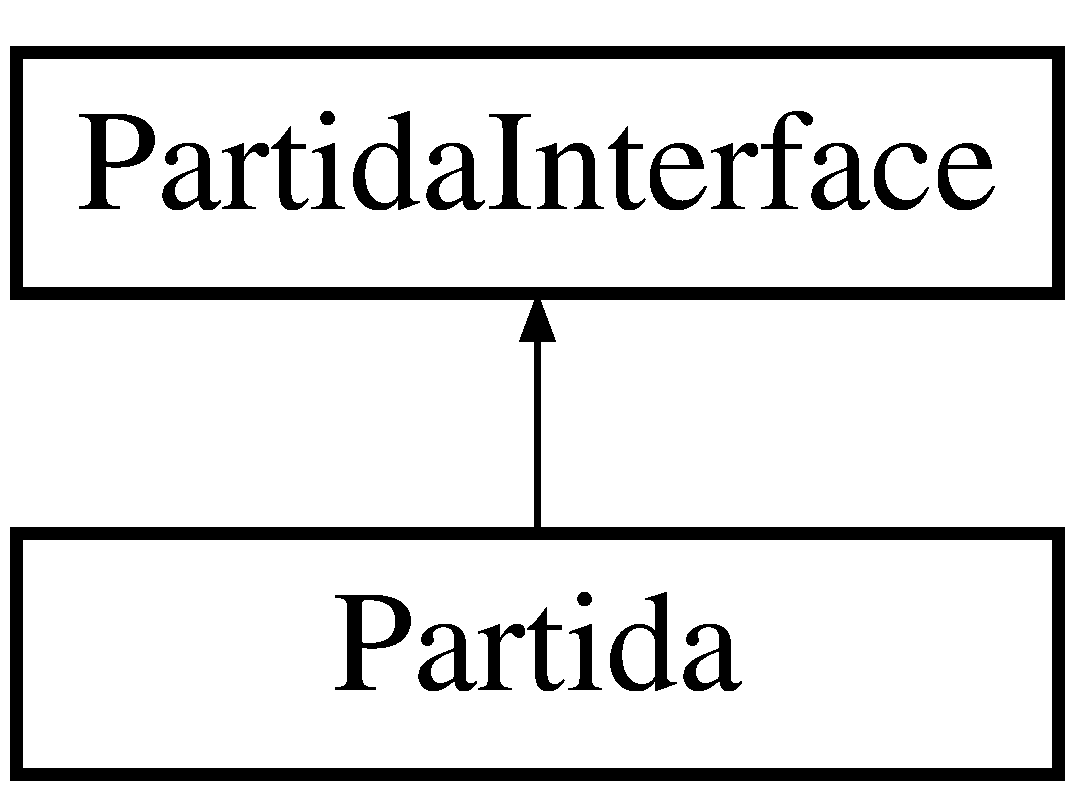
\includegraphics[height=2.000000cm]{classPartidaInterface}
\end{center}
\end{figure}
\subsection*{Public Member Functions}
\begin{DoxyCompactItemize}
\item 
\hypertarget{classPartidaInterface_a1190634ccd9ce1b78a83ef0e68c67bc5}{virtual void {\bfseries add\-Usuario} (\hyperlink{classThreadSocket}{Thread\-Socket} $\ast$u, Json\-::\-Value \&user)=0}\label{classPartidaInterface_a1190634ccd9ce1b78a83ef0e68c67bc5}

\item 
\hypertarget{classPartidaInterface_a41823671d949f4c2b9abbaca3709ca63}{virtual void {\bfseries rm\-Usuario} (\hyperlink{classThreadSocket}{Thread\-Socket} $\ast$u)=0}\label{classPartidaInterface_a41823671d949f4c2b9abbaca3709ca63}

\item 
virtual int \hyperlink{classPartidaInterface_a72c79ab5c06e2ec804260dc98a977e60}{mensaje} (Json\-::\-Value \&m, \hyperlink{classThreadSocket}{Thread\-Socket} $\ast$u)=0
\item 
\hypertarget{classPartidaInterface_af3e878d3e1de9d64f17e12b32dcc7643}{virtual int {\bfseries get\-Nivel} ()=0}\label{classPartidaInterface_af3e878d3e1de9d64f17e12b32dcc7643}

\item 
\hypertarget{classPartidaInterface_a8788de756e14af6febdf8bd44f8ff02b}{virtual int {\bfseries get\-Usuarios} ()=0}\label{classPartidaInterface_a8788de756e14af6febdf8bd44f8ff02b}

\item 
\hypertarget{classPartidaInterface_aa3b96356d4b96b799900c9425da251ba}{virtual int {\bfseries get\-Max\-Usuarios} ()=0}\label{classPartidaInterface_aa3b96356d4b96b799900c9425da251ba}

\item 
\hypertarget{classPartidaInterface_ac6b479769dd8d53ced7e0cbc147ca4d5}{virtual Partida\-Estado {\bfseries get\-Estado} ()=0}\label{classPartidaInterface_ac6b479769dd8d53ced7e0cbc147ca4d5}

\item 
\hypertarget{classPartidaInterface_a0287b2294f48e9bbda0173df9544964c}{virtual std\-::string {\bfseries get\-Nombre} ()=0}\label{classPartidaInterface_a0287b2294f48e9bbda0173df9544964c}

\end{DoxyCompactItemize}


\subsection{Detailed Description}
Interface de partida, para evitar referencia circular. 

\subsection{Member Function Documentation}
\hypertarget{classPartidaInterface_a72c79ab5c06e2ec804260dc98a977e60}{\index{Partida\-Interface@{Partida\-Interface}!mensaje@{mensaje}}
\index{mensaje@{mensaje}!PartidaInterface@{Partida\-Interface}}
\subsubsection[{mensaje}]{\setlength{\rightskip}{0pt plus 5cm}virtual int Partida\-Interface\-::mensaje (
\begin{DoxyParamCaption}
\item[{Json\-::\-Value \&}]{m, }
\item[{{\bf Thread\-Socket} $\ast$}]{u}
\end{DoxyParamCaption}
)\hspace{0.3cm}{\ttfamily [pure virtual]}}}\label{classPartidaInterface_a72c79ab5c06e2ec804260dc98a977e60}
Se le pasan todos los E\-V\-E\-N\-T\-\_\-\-G\-A\-M\-E\-\_\-\-M\-I\-S\-C. Devuelve 0 si todo bien, o 1, si el usuario se desconecto (saca usuario-\/$>$partida). La parida se debe encargar de toda la borrada de datos de si misma. 

Implemented in \hyperlink{classPartida_af5f9e1261116d75042a87ad0b5990700}{Partida}.



The documentation for this class was generated from the following file\-:\begin{DoxyCompactItemize}
\item 
server.\-partida\-\_\-interface.\-h\end{DoxyCompactItemize}

\hypertarget{classServer}{\section{Server Class Reference}
\label{classServer}\index{Server@{Server}}
}


{\ttfamily \#include $<$server.\-server.\-h$>$}

Inheritance diagram for Server\-:\begin{figure}[H]
\begin{center}
\leavevmode
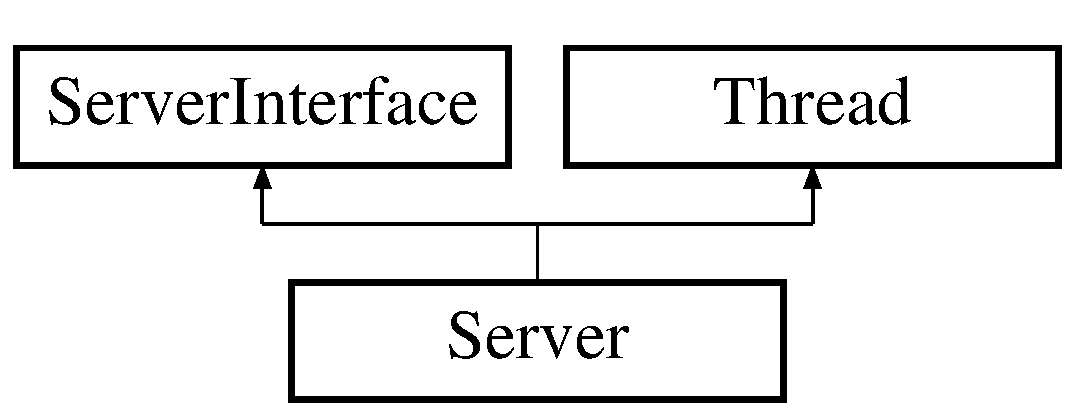
\includegraphics[height=2.000000cm]{classServer}
\end{center}
\end{figure}
\subsection*{Public Member Functions}
\begin{DoxyCompactItemize}
\item 
\hypertarget{classServer_a7d1fe6ba5f0fe9190a4f039662ea0e85}{{\bfseries Server} (int port)}\label{classServer_a7d1fe6ba5f0fe9190a4f039662ea0e85}

\item 
\hypertarget{classServer_ab16debc269fb57db4976b7199076b899}{void {\bfseries remove\-Client} (\hyperlink{classThreadSocket}{Thread\-Socket} $\ast$cli)}\label{classServer_ab16debc269fb57db4976b7199076b899}

\item 
\hypertarget{classServer_a710a8ebac1aa95fbb02458483b3bb408}{\hyperlink{classPartidaInterface}{Partida\-Interface} $\ast$ {\bfseries new\-Partida} (int nivel, std\-::string \&nombre)}\label{classServer_a710a8ebac1aa95fbb02458483b3bb408}

\item 
void \hyperlink{classServer_a1a5e9b3a3a6e4fc697163ab461fb11c6}{remove\-Partida} (\hyperlink{classPartidaInterface}{Partida\-Interface} $\ast$p)
\item 
virtual void \hyperlink{classServer_adf00f10f95cf9b49761475c73caead06}{list\-Partidas} (int nivel, Json\-::\-Value \&parts)
\item 
\hypertarget{classServer_a2af125bb682122c14979d9ead546b1a5}{virtual \hyperlink{classPartidaInterface}{Partida\-Interface} $\ast$ {\bfseries connect\-Partidas} (long id)}\label{classServer_a2af125bb682122c14979d9ead546b1a5}

\item 
\hypertarget{classServer_a83eef32fcef955048cc7ba7d35ff7552}{void {\bfseries end} ()}\label{classServer_a83eef32fcef955048cc7ba7d35ff7552}

\end{DoxyCompactItemize}
\subsection*{Protected Member Functions}
\begin{DoxyCompactItemize}
\item 
\hypertarget{classServer_a481bc16ea121723ce0fbc0af843a3648}{void {\bfseries add\-Client} (\hyperlink{classThreadUsuario}{Thread\-Usuario} $\ast$cli)}\label{classServer_a481bc16ea121723ce0fbc0af843a3648}

\item 
\hypertarget{classServer_a707bd1cc6a43cb4a444fc5e2bec11533}{int {\bfseries main} ()}\label{classServer_a707bd1cc6a43cb4a444fc5e2bec11533}

\item 
\hypertarget{classServer_a6defda6a554b733c833987f85d2e509d}{virtual void $\ast$ {\bfseries run} ()}\label{classServer_a6defda6a554b733c833987f85d2e509d}

\end{DoxyCompactItemize}
\subsection*{Protected Attributes}
\begin{DoxyCompactItemize}
\item 
\hypertarget{classServer_a926c9dae229a62b6d33fdbb41dca6d82}{int {\bfseries port}}\label{classServer_a926c9dae229a62b6d33fdbb41dca6d82}

\item 
std\-::vector$<$ \hyperlink{classThreadUsuario}{Thread\-Usuario} $\ast$ $>$ \hyperlink{classServer_a295a2426aee46c5a82085fa5b70828c2}{clientes}
\item 
\hypertarget{classServer_a8f5063d67347091cd0d210fafe8d5cf1}{std\-::vector$<$ \hyperlink{classPartida}{Partida} $\ast$ $>$ {\bfseries partidas}}\label{classServer_a8f5063d67347091cd0d210fafe8d5cf1}

\item 
\hypertarget{classServer_aba30475b0b0ec7c39bc70c852c0d582e}{\hyperlink{classTCPSocketListener}{T\-C\-P\-Socket\-Listener} {\bfseries sock}}\label{classServer_aba30475b0b0ec7c39bc70c852c0d582e}

\item 
\hypertarget{classServer_ad33f68ad78c3045c49dcf066afb5c102}{\hyperlink{classMutex}{Mutex} {\bfseries clientes\-Lock}}\label{classServer_ad33f68ad78c3045c49dcf066afb5c102}

\item 
\hypertarget{classServer_a757a2d8318b9443d168bf4c772c76260}{\hyperlink{classMutex}{Mutex} {\bfseries partidas\-Lock}}\label{classServer_a757a2d8318b9443d168bf4c772c76260}

\end{DoxyCompactItemize}


\subsection{Detailed Description}
Clase de servidor. Esta bloqueada escuchando, cada vez que se conecta un cliente se lanza un nuevo thread con el socket creado (se lanza un \hyperlink{classThreadUsuario}{Thread\-Usuario}) 

\subsection{Member Function Documentation}
\hypertarget{classServer_adf00f10f95cf9b49761475c73caead06}{\index{Server@{Server}!list\-Partidas@{list\-Partidas}}
\index{list\-Partidas@{list\-Partidas}!Server@{Server}}
\subsubsection[{list\-Partidas}]{\setlength{\rightskip}{0pt plus 5cm}void Server\-::list\-Partidas (
\begin{DoxyParamCaption}
\item[{int}]{nivel, }
\item[{Json\-::\-Value \&}]{parts}
\end{DoxyParamCaption}
)\hspace{0.3cm}{\ttfamily [virtual]}}}\label{classServer_adf00f10f95cf9b49761475c73caead06}
Devuelve un J\-S\-O\-N con las partidas de nivel menor o igual al especificado. 

Implements \hyperlink{classServerInterface}{Server\-Interface}.

\hypertarget{classServer_a1a5e9b3a3a6e4fc697163ab461fb11c6}{\index{Server@{Server}!remove\-Partida@{remove\-Partida}}
\index{remove\-Partida@{remove\-Partida}!Server@{Server}}
\subsubsection[{remove\-Partida}]{\setlength{\rightskip}{0pt plus 5cm}void Server\-::remove\-Partida (
\begin{DoxyParamCaption}
\item[{{\bf Partida\-Interface} $\ast$}]{p}
\end{DoxyParamCaption}
)\hspace{0.3cm}{\ttfamily [virtual]}}}\label{classServer_a1a5e9b3a3a6e4fc697163ab461fb11c6}
Remueve partida de la lista 

Implements \hyperlink{classServerInterface}{Server\-Interface}.



\subsection{Member Data Documentation}
\hypertarget{classServer_a295a2426aee46c5a82085fa5b70828c2}{\index{Server@{Server}!clientes@{clientes}}
\index{clientes@{clientes}!Server@{Server}}
\subsubsection[{clientes}]{\setlength{\rightskip}{0pt plus 5cm}std\-::vector$<${\bf Thread\-Usuario}$\ast$$>$ Server\-::clientes\hspace{0.3cm}{\ttfamily [protected]}}}\label{classServer_a295a2426aee46c5a82085fa5b70828c2}
Guarda todos los threads de los usuarios corriendo 

The documentation for this class was generated from the following files\-:\begin{DoxyCompactItemize}
\item 
server.\-server.\-h\item 
server.\-server.\-cpp\end{DoxyCompactItemize}

\hypertarget{classServerInterface}{\section{Server\-Interface Class Reference}
\label{classServerInterface}\index{Server\-Interface@{Server\-Interface}}
}
Inheritance diagram for Server\-Interface\-:\begin{figure}[H]
\begin{center}
\leavevmode
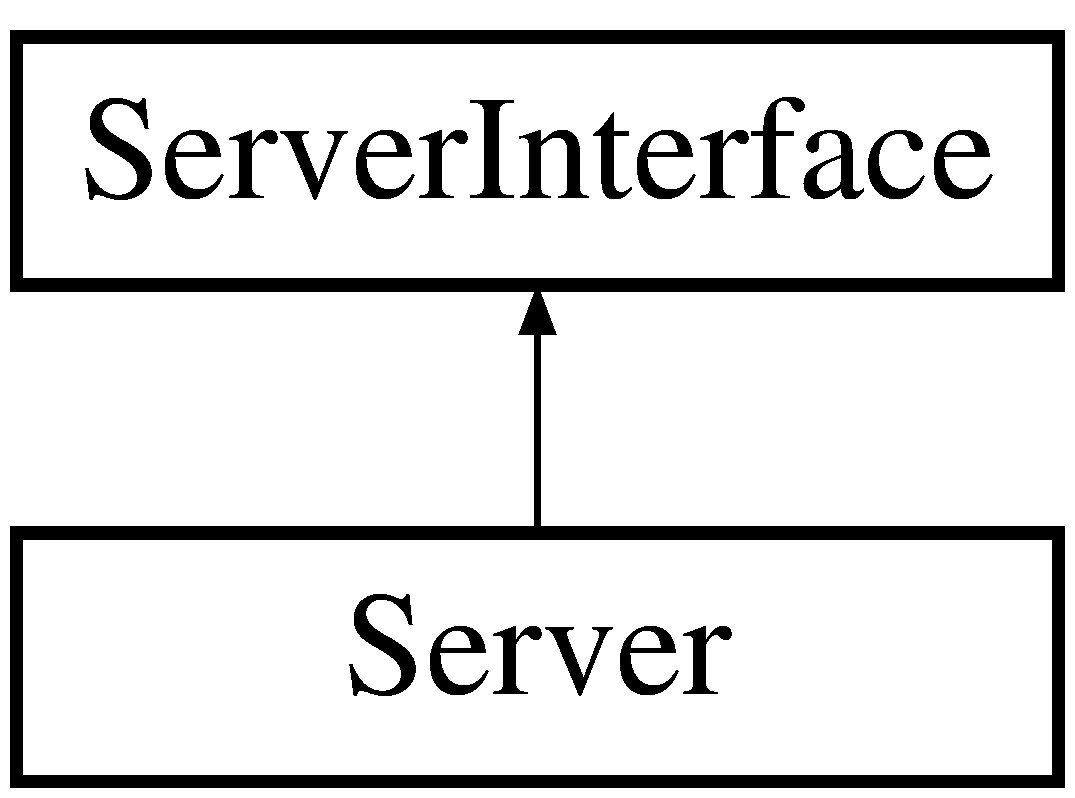
\includegraphics[height=2.000000cm]{classServerInterface}
\end{center}
\end{figure}
\subsection*{Public Member Functions}
\begin{DoxyCompactItemize}
\item 
\hypertarget{classServerInterface_a9f50fb72f2b1f039a5b0ed87fafe4446}{virtual void {\bfseries remove\-Client} (\hyperlink{classThreadSocket}{Thread\-Socket} $\ast$cli)=0}\label{classServerInterface_a9f50fb72f2b1f039a5b0ed87fafe4446}

\item 
\hypertarget{classServerInterface_a6dff7955b7dce57f18d8b5cb37602a67}{virtual \hyperlink{classPartidaInterface}{Partida\-Interface} $\ast$ {\bfseries new\-Partida} (int nivel, std\-::string \&nombre)=0}\label{classServerInterface_a6dff7955b7dce57f18d8b5cb37602a67}

\item 
\hypertarget{classServerInterface_ad17e40c4c3823ab6b52a9a82cfd55c4b}{virtual void {\bfseries remove\-Partida} (\hyperlink{classPartidaInterface}{Partida\-Interface} $\ast$p)=0}\label{classServerInterface_ad17e40c4c3823ab6b52a9a82cfd55c4b}

\item 
\hypertarget{classServerInterface_ac1a109664797797594773dd4881230cb}{virtual void {\bfseries list\-Partidas} (int nivel, Json\-::\-Value \&parts)=0}\label{classServerInterface_ac1a109664797797594773dd4881230cb}

\item 
\hypertarget{classServerInterface_a0ef2aa76b2b0c254ae96a8e737f9ef49}{virtual \hyperlink{classPartidaInterface}{Partida\-Interface} $\ast$ {\bfseries connect\-Partidas} (long id)=0}\label{classServerInterface_a0ef2aa76b2b0c254ae96a8e737f9ef49}

\end{DoxyCompactItemize}


The documentation for this class was generated from the following file\-:\begin{DoxyCompactItemize}
\item 
server.\-server\-\_\-interface.\-h\end{DoxyCompactItemize}

\hypertarget{classSocket}{\section{Socket Class Reference}
\label{classSocket}\index{Socket@{Socket}}
}
Inheritance diagram for Socket\-:\begin{figure}[H]
\begin{center}
\leavevmode
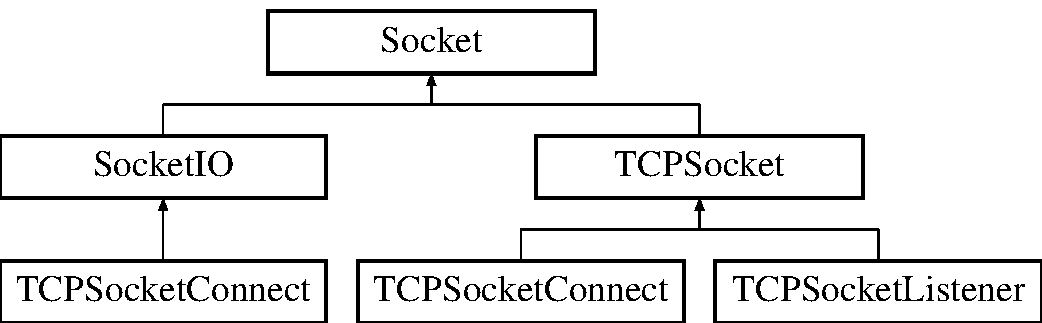
\includegraphics[height=3.000000cm]{classSocket}
\end{center}
\end{figure}
\subsection*{Public Member Functions}
\begin{DoxyCompactItemize}
\item 
\hypertarget{classSocket_a41a26876313a89591552648677320602}{int {\bfseries shutdown} ()}\label{classSocket_a41a26876313a89591552648677320602}

\item 
\hypertarget{classSocket_a8ca1576b3de3ff4685101c833ad3418c}{int {\bfseries shutdown} (int how)}\label{classSocket_a8ca1576b3de3ff4685101c833ad3418c}

\end{DoxyCompactItemize}
\subsection*{Protected Member Functions}
\begin{DoxyCompactItemize}
\item 
\hypertarget{classSocket_a7b44c495bfeddf489649464e8d5445e1}{struct sockaddr\-\_\-in $\ast$ {\bfseries ip2struct} (const int port, const std\-::string \&ip)}\label{classSocket_a7b44c495bfeddf489649464e8d5445e1}

\item 
\hypertarget{classSocket_ae3fd77c7223c9489b3b170a02d5fd385}{struct sockaddr\-\_\-in $\ast$ {\bfseries ip2struct} (const std\-::string \&port, const std\-::string \&ip)}\label{classSocket_ae3fd77c7223c9489b3b170a02d5fd385}

\item 
\hypertarget{classSocket_a6cb5eb88e856b00e1adb3cce809634f8}{struct sockaddr\-\_\-in $\ast$ {\bfseries ip2struct} (const std\-::string \&ipport)}\label{classSocket_a6cb5eb88e856b00e1adb3cce809634f8}

\end{DoxyCompactItemize}
\subsection*{Protected Attributes}
\begin{DoxyCompactItemize}
\item 
\hypertarget{classSocket_a25dd8cf38a7a8742858f5b3193deeb15}{unsigned int {\bfseries fd}}\label{classSocket_a25dd8cf38a7a8742858f5b3193deeb15}

\end{DoxyCompactItemize}


The documentation for this class was generated from the following files\-:\begin{DoxyCompactItemize}
\item 
common.\-socket.\-h\item 
common.\-socket.\-cpp\end{DoxyCompactItemize}

\hypertarget{classSocketIO}{\section{Socket\-I\-O Class Reference}
\label{classSocketIO}\index{Socket\-I\-O@{Socket\-I\-O}}
}


{\ttfamily \#include $<$common.\-socket\-\_\-io.\-h$>$}

Inheritance diagram for Socket\-I\-O\-:\begin{figure}[H]
\begin{center}
\leavevmode
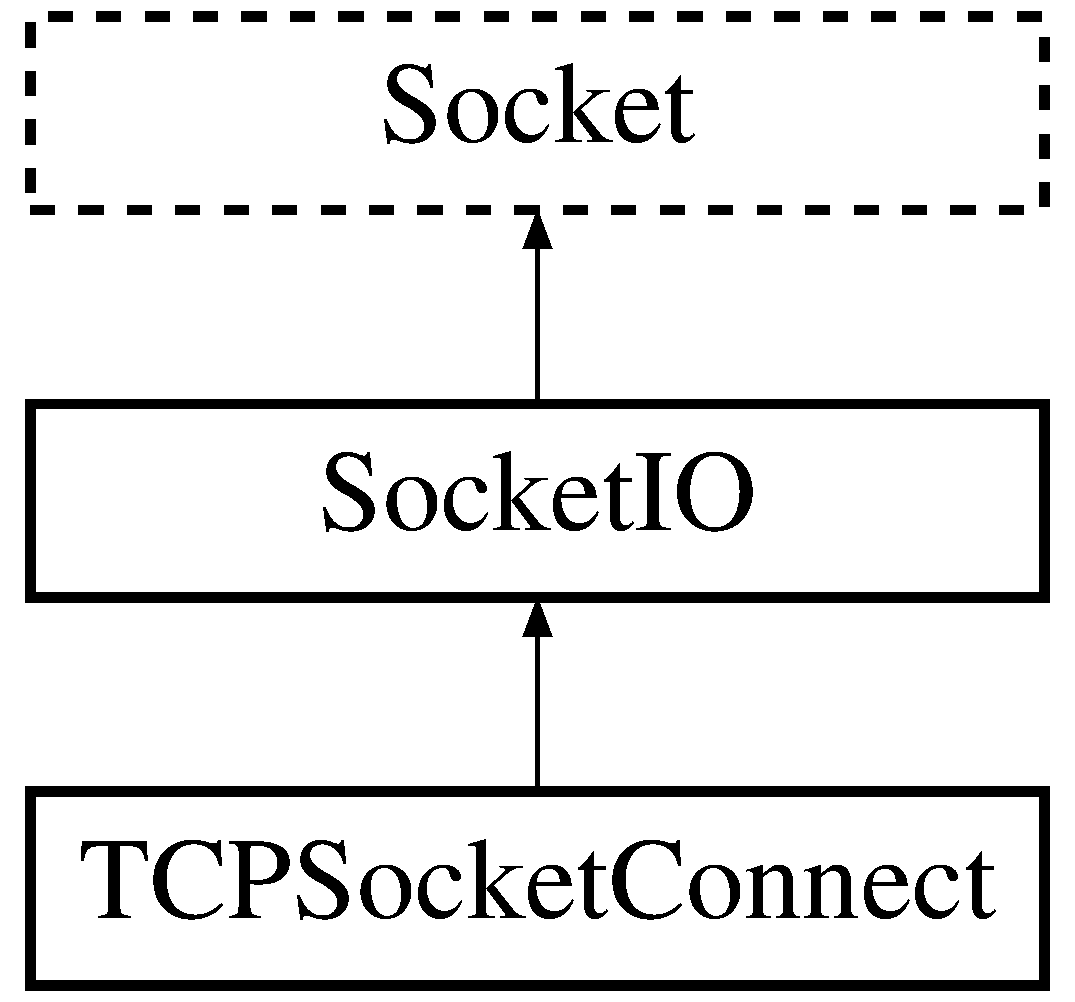
\includegraphics[height=3.000000cm]{classSocketIO}
\end{center}
\end{figure}
\subsection*{Public Member Functions}
\begin{DoxyCompactItemize}
\item 
\hypertarget{classSocketIO_a6fab1f7899e781b7fea87fbdc6c0e353}{{\bfseries Socket\-I\-O} (unsigned int fd)}\label{classSocketIO_a6fab1f7899e781b7fea87fbdc6c0e353}

\item 
int \hyperlink{classSocketIO_aa9f50be5a8b12fbab93893de212b8a59}{read} (Json\-::\-Value \&data, const std\-::string \&key, bool check=true)
\item 
int \hyperlink{classSocketIO_a29877c264b1d6c116d07e0a9f76c5373}{write} (const Json\-::\-Value \&data, const std\-::string \&key)
\end{DoxyCompactItemize}
\subsection*{Additional Inherited Members}


\subsection{Detailed Description}
\hyperlink{classSocket}{Socket} de entrada y salida. Implementa metodos de escribir y leer con firma. 

\subsection{Member Function Documentation}
\hypertarget{classSocketIO_aa9f50be5a8b12fbab93893de212b8a59}{\index{Socket\-I\-O@{Socket\-I\-O}!read@{read}}
\index{read@{read}!SocketIO@{Socket\-I\-O}}
\subsubsection[{read}]{\setlength{\rightskip}{0pt plus 5cm}int Socket\-I\-O\-::read (
\begin{DoxyParamCaption}
\item[{Json\-::\-Value \&}]{data, }
\item[{const std\-::string \&}]{key, }
\item[{bool}]{check = {\ttfamily true}}
\end{DoxyParamCaption}
)}}\label{classSocketIO_aa9f50be5a8b12fbab93893de212b8a59}
read\-: lee mensaje. Lee mensaje de socket. Primero lee prefijo de longitud, dependiendo de eso, lee el mensaje, y despues lee la firma, la validacion de la misma es opcional, pero siempre se la leera. El metodo se encarga de la transformacion de la data json entrante en objeto. En el caso de haber una firma invalida, se saldra con error, pero se devolvera por data el json recibido. 
\begin{DoxyParams}[1]{Parameters}
\mbox{\tt out}  & {\em data} & informacion proveniente del socket. \\
\hline
\mbox{\tt in}  & {\em key} & llave usada para la comprobacion de la firma. \\
\hline
\mbox{\tt in}  & {\em check} & opcional, (true por defecto) si es verdadero se chequeara la firma. \\
\hline
\end{DoxyParams}
\begin{DoxyReturn}{Returns}
0 ok, -\/1 para cualqier error de lectura de socket, 1 para error de validacion de firma, 2 para problemas de parseo de json. 
\end{DoxyReturn}
\hypertarget{classSocketIO_a29877c264b1d6c116d07e0a9f76c5373}{\index{Socket\-I\-O@{Socket\-I\-O}!write@{write}}
\index{write@{write}!SocketIO@{Socket\-I\-O}}
\subsubsection[{write}]{\setlength{\rightskip}{0pt plus 5cm}int Socket\-I\-O\-::write (
\begin{DoxyParamCaption}
\item[{const Json\-::\-Value \&}]{data, }
\item[{const std\-::string \&}]{key}
\end{DoxyParamCaption}
)}}\label{classSocketIO_a29877c264b1d6c116d07e0a9f76c5373}
write\-: envia el mensaje. Agrega prefijo de longitud (en bytes) y firma del mensaje. El prefijo de longitud es un uint32\-\_\-t que esta puesto con hton, despues viene el mensaje (en json) y por ultimo la firma del mensaje\begin{DoxySeeAlso}{See Also}
hmac\-\_\-msje(). El largo se refiere solo al largo del mensaje, no incluye el largo de la firma que siempre sera el mismo. El orden es $<$prefijo\-\_\-longitud$>$$<$mensaje$>$$<$firma$>$. El metodo se encarga de serializar. 
\end{DoxySeeAlso}

\begin{DoxyParams}[1]{Parameters}
\mbox{\tt in}  & {\em data} & data a enviar \\
\hline
\mbox{\tt in}  & {\em key} & llave para la firma \\
\hline
\end{DoxyParams}
\begin{DoxyReturn}{Returns}
codigo de error, 0 ok, resto error. 
\end{DoxyReturn}


The documentation for this class was generated from the following files\-:\begin{DoxyCompactItemize}
\item 
common.\-socket\-\_\-io.\-h\item 
common.\-socket\-\_\-io.\-cpp\end{DoxyCompactItemize}

\hypertarget{classSoundPlayer}{\section{Sound\-Player Class Reference}
\label{classSoundPlayer}\index{Sound\-Player@{Sound\-Player}}
}


{\ttfamily \#include $<$cliente.\-sound\-\_\-player.\-h$>$}

\subsection*{Static Public Member Functions}
\begin{DoxyCompactItemize}
\item 
static bool \hyperlink{classSoundPlayer_abe94eb635c2c94b9ae4e852b35a2402f}{play} (const std\-::string \&str)
\item 
\hypertarget{classSoundPlayer_a8a59acf29748daccddc07c0595ce834e}{static bool {\bfseries play} (const char $\ast$str)}\label{classSoundPlayer_a8a59acf29748daccddc07c0595ce834e}

\end{DoxyCompactItemize}
\subsection*{Protected Member Functions}
\begin{DoxyCompactItemize}
\item 
\hypertarget{classSoundPlayer_a7a15151efe24e566febd36238ff6056a}{void {\bfseries thread\-\_\-play} (int fd, int sample\-\_\-rate, int seconds)}\label{classSoundPlayer_a7a15151efe24e566febd36238ff6056a}

\end{DoxyCompactItemize}
\subsection*{Static Protected Member Functions}
\begin{DoxyCompactItemize}
\item 
\hypertarget{classSoundPlayer_a9bda2f100c481f1142712f03e94ff3d0}{static bool {\bfseries play\-\_\-wave} (const std\-::string \&str)}\label{classSoundPlayer_a9bda2f100c481f1142712f03e94ff3d0}

\item 
\hypertarget{classSoundPlayer_ad7ae434f37549077a8296af13dbbeed5}{static void $\ast$ {\bfseries wav\-\_\-runner} (void $\ast$arg)}\label{classSoundPlayer_ad7ae434f37549077a8296af13dbbeed5}

\end{DoxyCompactItemize}
\subsection*{Static Protected Attributes}
\begin{DoxyCompactItemize}
\item 
static std\-::map$<$ std\-::string, \\*
std\-::time\-\_\-t $>$ \hyperlink{classSoundPlayer_aa597752d2e520979b12e026fdd9c116d}{archs}
\end{DoxyCompactItemize}


\subsection{Detailed Description}
Clase singleton usada para reproducir sonidos. No es threadsafe, solo se puede ejecutar desde un thread. Si se mandan a reproducir dos sonidos iguales en el mismo segundo, solo reproduce el primero. 

\subsection{Member Function Documentation}
\hypertarget{classSoundPlayer_abe94eb635c2c94b9ae4e852b35a2402f}{\index{Sound\-Player@{Sound\-Player}!play@{play}}
\index{play@{play}!SoundPlayer@{Sound\-Player}}
\subsubsection[{play}]{\setlength{\rightskip}{0pt plus 5cm}bool Sound\-Player\-::play (
\begin{DoxyParamCaption}
\item[{const std\-::string \&}]{str}
\end{DoxyParamCaption}
)\hspace{0.3cm}{\ttfamily [static]}}}\label{classSoundPlayer_abe94eb635c2c94b9ae4e852b35a2402f}
Funciones usadas para reproducir. 

\subsection{Member Data Documentation}
\hypertarget{classSoundPlayer_aa597752d2e520979b12e026fdd9c116d}{\index{Sound\-Player@{Sound\-Player}!archs@{archs}}
\index{archs@{archs}!SoundPlayer@{Sound\-Player}}
\subsubsection[{archs}]{\setlength{\rightskip}{0pt plus 5cm}std\-::map$<$ std\-::string, std\-::time\-\_\-t $>$ Sound\-Player\-::archs\hspace{0.3cm}{\ttfamily [static]}, {\ttfamily [protected]}}}\label{classSoundPlayer_aa597752d2e520979b12e026fdd9c116d}
Guarda usando de clave el path, la hora de cunado fue reproducido. Se usa para ignorar archivos iguales si se reproducen en el mismo momento 

The documentation for this class was generated from the following files\-:\begin{DoxyCompactItemize}
\item 
cliente.\-sound\-\_\-player.\-h\item 
cliente.\-sound\-\_\-player.\-cpp\end{DoxyCompactItemize}

\hypertarget{classStar}{\section{Star Class Reference}
\label{classStar}\index{Star@{Star}}
}
Inheritance diagram for Star\-:\begin{figure}[H]
\begin{center}
\leavevmode
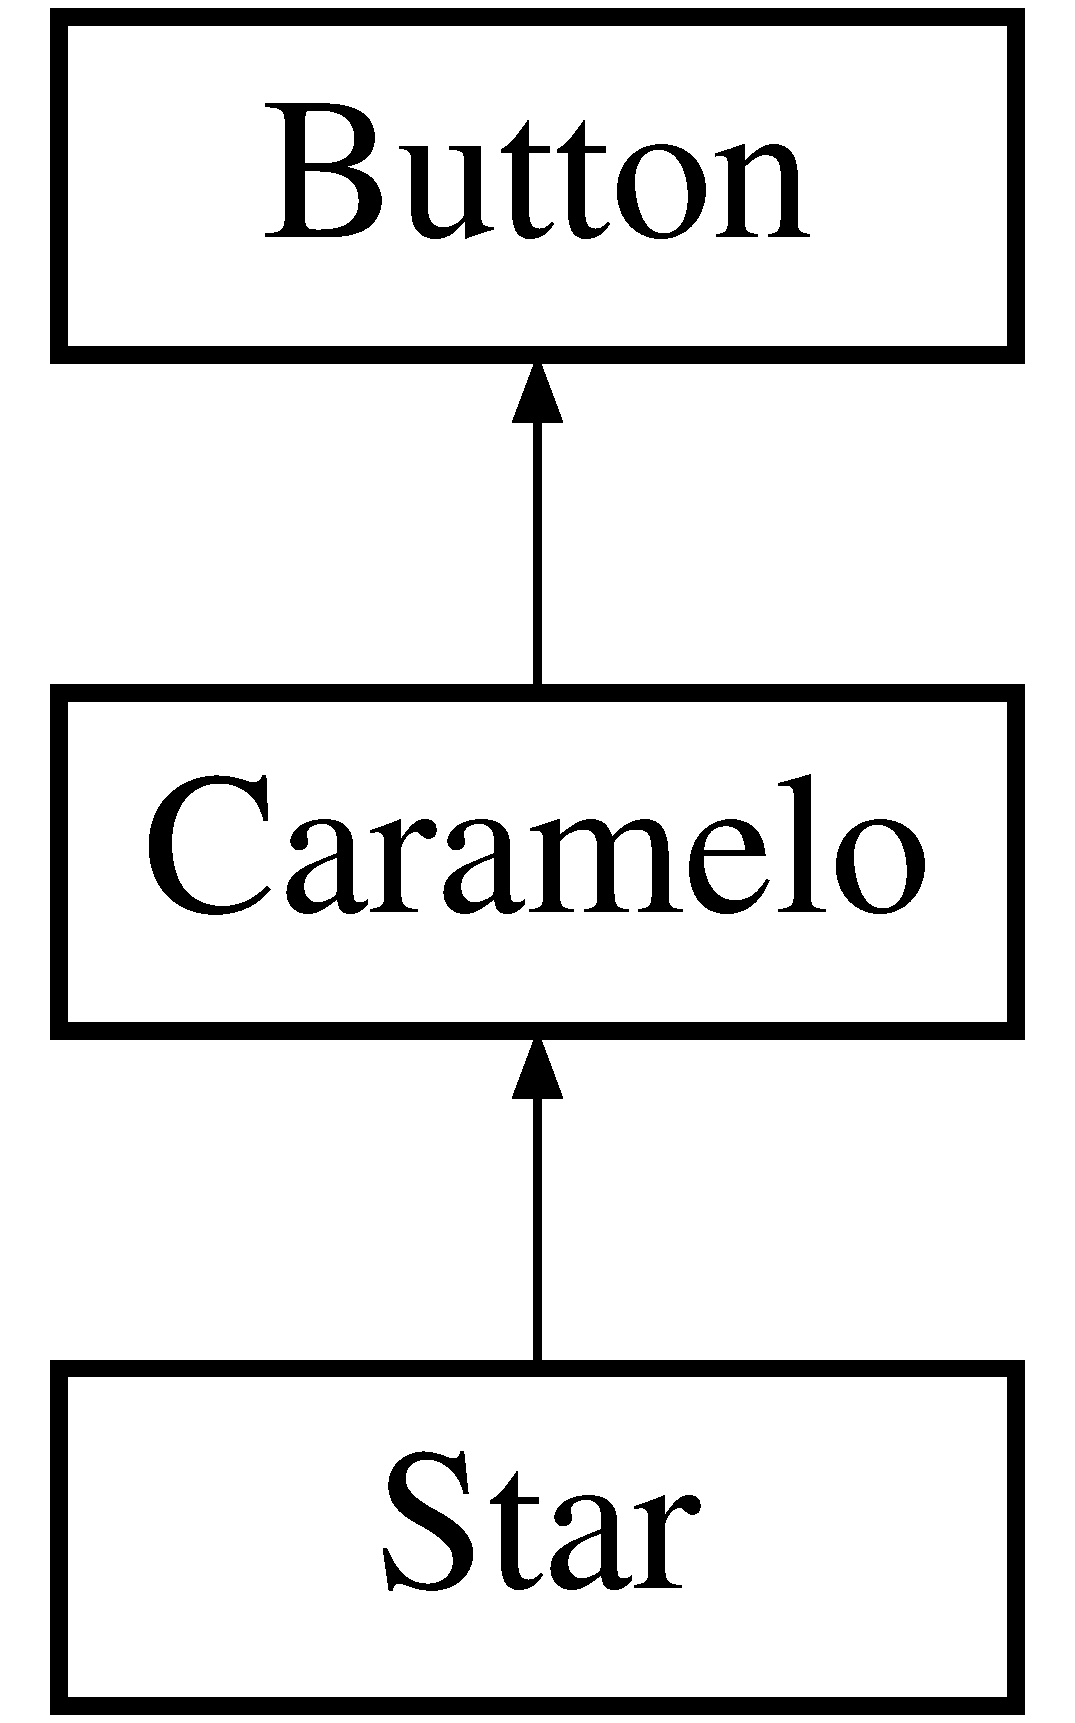
\includegraphics[height=3.000000cm]{classStar}
\end{center}
\end{figure}
\subsection*{Public Member Functions}
\begin{DoxyCompactItemize}
\item 
\hypertarget{classStar_a87aed798f84d9e121430ce9675074937}{{\bfseries Star} (int id\-Caramelo, const std\-::string \&img\-Dir, int i, int j)}\label{classStar_a87aed798f84d9e121430ce9675074937}

\item 
\hypertarget{classStar_aafa59ff0555adfb746cc40c58847fa30}{bool {\bfseries mover} ()}\label{classStar_aafa59ff0555adfb746cc40c58847fa30}

\end{DoxyCompactItemize}


The documentation for this class was generated from the following file\-:\begin{DoxyCompactItemize}
\item 
cliente.\-star.\-h\end{DoxyCompactItemize}

\hypertarget{classTablero}{\section{Tablero Class Reference}
\label{classTablero}\index{Tablero@{Tablero}}
}


{\ttfamily \#include $<$tablero.\-h$>$}

\subsection*{Public Types}
\begin{DoxyCompactItemize}
\item 
typedef sigc\-::signal$<$ void $>$ \hyperlink{classTablero_a1c847f6d745139e22ca87a32f82ded14}{type\-\_\-signal\-\_\-uncheck}
\end{DoxyCompactItemize}
\subsection*{Public Member Functions}
\begin{DoxyCompactItemize}
\item 
\hyperlink{classTablero_ada8ba5e6781488793f2f78c3799aa4ff}{Tablero} (Glib\-::\-Ref\-Ptr$<$ Gtk\-::\-Builder $>$ \&builder)
\item 
void \hyperlink{classTablero_a58e80bae3f019987b9283723f8a57b84}{on\-\_\-adj\-Cols\-\_\-changed\-\_\-tablero} (Gtk\-::\-Spin\-Button $\ast$spinbutton, int id)
\item 
void \hyperlink{classTablero_afacc7a7dd1f42590e39b87cae48e3275}{on\-\_\-cordx\-\_\-changed} (Gtk\-::\-Spin\-Button $\ast$spin\-\_\-x)
\item 
void \hyperlink{classTablero_a2e94fb8a39b63af67fc1d2d00eb40bb3}{on\-\_\-cordy\-\_\-changed} (Gtk\-::\-Spin\-Button $\ast$spin\-\_\-y)
\item 
void \hyperlink{classTablero_ab7f1519be16814243a5b425600dd59a0}{on\-\_\-adj\-\_\-changed\-\_\-tablero} (Gtk\-::\-Spin\-Button $\ast$spinbutton, int id)
\item 
void \hyperlink{classTablero_acdc841e43131788e8d722f341d2df174}{on\-\_\-image\-\_\-changed\-\_\-tablero} (Gtk\-::\-File\-Chooser $\ast$file\-Chooser)
\item 
void \hyperlink{classTablero_a910b04b2d9807d8618b2e176942da950}{on\-\_\-image\-\_\-fondo\-\_\-changed\-\_\-tablero} (Gtk\-::\-File\-Chooser $\ast$file\-Chooser)
\item 
void \hyperlink{classTablero_a2e329c07dbc1a33793958eb8b192bbc3}{on\-\_\-check\-\_\-button\-\_\-tablero} ()
\item 
void \hyperlink{classTablero_a17f4eadec115ef30e08a45d9b26a6fc4}{json\-Celdas} (Json\-::\-Value \&nivel, const std\-::string \&nombre)
\item 
void \hyperlink{classTablero_a47c278b608b5e1dd22aeafcdba0ea0f2}{json\-Columnas} (Json\-::\-Value \&nivel, const std\-::string \&nombre)
\item 
\hypertarget{classTablero_aefdae69f836627a44aec877940919099}{\hyperlink{classTablero_a1c847f6d745139e22ca87a32f82ded14}{type\-\_\-signal\-\_\-uncheck} {\bfseries signal\-\_\-uncheck} ()}\label{classTablero_aefdae69f836627a44aec877940919099}

\end{DoxyCompactItemize}


\subsection{Detailed Description}
\hyperlink{classTablero}{Tablero} de juego . 

\subsection{Member Typedef Documentation}
\hypertarget{classTablero_a1c847f6d745139e22ca87a32f82ded14}{\index{Tablero@{Tablero}!type\-\_\-signal\-\_\-uncheck@{type\-\_\-signal\-\_\-uncheck}}
\index{type\-\_\-signal\-\_\-uncheck@{type\-\_\-signal\-\_\-uncheck}!Tablero@{Tablero}}
\subsubsection[{type\-\_\-signal\-\_\-uncheck}]{\setlength{\rightskip}{0pt plus 5cm}typedef sigc\-::signal$<$ void $>$ {\bf Tablero\-::type\-\_\-signal\-\_\-uncheck}}}\label{classTablero_a1c847f6d745139e22ca87a32f82ded14}
Senal que se emite despues de hacer click 

\subsection{Constructor \& Destructor Documentation}
\hypertarget{classTablero_ada8ba5e6781488793f2f78c3799aa4ff}{\index{Tablero@{Tablero}!Tablero@{Tablero}}
\index{Tablero@{Tablero}!Tablero@{Tablero}}
\subsubsection[{Tablero}]{\setlength{\rightskip}{0pt plus 5cm}Tablero\-::\-Tablero (
\begin{DoxyParamCaption}
\item[{Glib\-::\-Ref\-Ptr$<$ Gtk\-::\-Builder $>$ \&}]{builder}
\end{DoxyParamCaption}
)\hspace{0.3cm}{\ttfamily [explicit]}}}\label{classTablero_ada8ba5e6781488793f2f78c3799aa4ff}
Constructor de tablero. 
\begin{DoxyParams}{Parameters}
{\em builder,\-:} & Utilizado para levantar widgets del archivo de glade \\
\hline
\end{DoxyParams}


\subsection{Member Function Documentation}
\hypertarget{classTablero_a17f4eadec115ef30e08a45d9b26a6fc4}{\index{Tablero@{Tablero}!json\-Celdas@{json\-Celdas}}
\index{json\-Celdas@{json\-Celdas}!Tablero@{Tablero}}
\subsubsection[{json\-Celdas}]{\setlength{\rightskip}{0pt plus 5cm}void Tablero\-::json\-Celdas (
\begin{DoxyParamCaption}
\item[{Json\-::\-Value \&}]{nivel, }
\item[{const std\-::string \&}]{nombre}
\end{DoxyParamCaption}
)}}\label{classTablero_a17f4eadec115ef30e08a45d9b26a6fc4}
Serializa la informacion de las celdas. \hypertarget{classTablero_a47c278b608b5e1dd22aeafcdba0ea0f2}{\index{Tablero@{Tablero}!json\-Columnas@{json\-Columnas}}
\index{json\-Columnas@{json\-Columnas}!Tablero@{Tablero}}
\subsubsection[{json\-Columnas}]{\setlength{\rightskip}{0pt plus 5cm}void Tablero\-::json\-Columnas (
\begin{DoxyParamCaption}
\item[{Json\-::\-Value \&}]{nivel, }
\item[{const std\-::string \&}]{nombre}
\end{DoxyParamCaption}
)}}\label{classTablero_a47c278b608b5e1dd22aeafcdba0ea0f2}
Serializa la informacion de las celdas. \hypertarget{classTablero_ab7f1519be16814243a5b425600dd59a0}{\index{Tablero@{Tablero}!on\-\_\-adj\-\_\-changed\-\_\-tablero@{on\-\_\-adj\-\_\-changed\-\_\-tablero}}
\index{on\-\_\-adj\-\_\-changed\-\_\-tablero@{on\-\_\-adj\-\_\-changed\-\_\-tablero}!Tablero@{Tablero}}
\subsubsection[{on\-\_\-adj\-\_\-changed\-\_\-tablero}]{\setlength{\rightskip}{0pt plus 5cm}void Tablero\-::on\-\_\-adj\-\_\-changed\-\_\-tablero (
\begin{DoxyParamCaption}
\item[{Gtk\-::\-Spin\-Button $\ast$}]{spinbutton, }
\item[{int}]{id}
\end{DoxyParamCaption}
)}}\label{classTablero_ab7f1519be16814243a5b425600dd59a0}
Se encarga de poner probabilidades por celda. 
\begin{DoxyParams}{Parameters}
{\em spinbutton,\-:} & Spin\-Button que cambio. \\
\hline
{\em id,\-:} & Numero de Spin\-Button que cambio. \\
\hline
\end{DoxyParams}
\hypertarget{classTablero_a58e80bae3f019987b9283723f8a57b84}{\index{Tablero@{Tablero}!on\-\_\-adj\-Cols\-\_\-changed\-\_\-tablero@{on\-\_\-adj\-Cols\-\_\-changed\-\_\-tablero}}
\index{on\-\_\-adj\-Cols\-\_\-changed\-\_\-tablero@{on\-\_\-adj\-Cols\-\_\-changed\-\_\-tablero}!Tablero@{Tablero}}
\subsubsection[{on\-\_\-adj\-Cols\-\_\-changed\-\_\-tablero}]{\setlength{\rightskip}{0pt plus 5cm}void Tablero\-::on\-\_\-adj\-Cols\-\_\-changed\-\_\-tablero (
\begin{DoxyParamCaption}
\item[{Gtk\-::\-Spin\-Button $\ast$}]{spinbutton, }
\item[{int}]{id}
\end{DoxyParamCaption}
)}}\label{classTablero_a58e80bae3f019987b9283723f8a57b84}
Se encarga de poner probabilidades por columna cuando un spinbutton cambia de valor. 
\begin{DoxyParams}{Parameters}
{\em spinbutton,\-:} & Spinbutton que cambio de valor. \\
\hline
{\em id,\-:} & Numero de spinbutton que cambio de valor. \\
\hline
\end{DoxyParams}
\hypertarget{classTablero_a2e329c07dbc1a33793958eb8b192bbc3}{\index{Tablero@{Tablero}!on\-\_\-check\-\_\-button\-\_\-tablero@{on\-\_\-check\-\_\-button\-\_\-tablero}}
\index{on\-\_\-check\-\_\-button\-\_\-tablero@{on\-\_\-check\-\_\-button\-\_\-tablero}!Tablero@{Tablero}}
\subsubsection[{on\-\_\-check\-\_\-button\-\_\-tablero}]{\setlength{\rightskip}{0pt plus 5cm}void Tablero\-::on\-\_\-check\-\_\-button\-\_\-tablero (
\begin{DoxyParamCaption}
{}
\end{DoxyParamCaption}
)}}\label{classTablero_a2e329c07dbc1a33793958eb8b192bbc3}
Pone un hueco en la celda que este seleccionada. \hypertarget{classTablero_afacc7a7dd1f42590e39b87cae48e3275}{\index{Tablero@{Tablero}!on\-\_\-cordx\-\_\-changed@{on\-\_\-cordx\-\_\-changed}}
\index{on\-\_\-cordx\-\_\-changed@{on\-\_\-cordx\-\_\-changed}!Tablero@{Tablero}}
\subsubsection[{on\-\_\-cordx\-\_\-changed}]{\setlength{\rightskip}{0pt plus 5cm}void Tablero\-::on\-\_\-cordx\-\_\-changed (
\begin{DoxyParamCaption}
\item[{Gtk\-::\-Spin\-Button $\ast$}]{spin\-\_\-x}
\end{DoxyParamCaption}
)}}\label{classTablero_afacc7a7dd1f42590e39b87cae48e3275}
Guarda el valor de spin\-\_\-x que contiene la cantidad de filas seleccionada. \hypertarget{classTablero_a2e94fb8a39b63af67fc1d2d00eb40bb3}{\index{Tablero@{Tablero}!on\-\_\-cordy\-\_\-changed@{on\-\_\-cordy\-\_\-changed}}
\index{on\-\_\-cordy\-\_\-changed@{on\-\_\-cordy\-\_\-changed}!Tablero@{Tablero}}
\subsubsection[{on\-\_\-cordy\-\_\-changed}]{\setlength{\rightskip}{0pt plus 5cm}void Tablero\-::on\-\_\-cordy\-\_\-changed (
\begin{DoxyParamCaption}
\item[{Gtk\-::\-Spin\-Button $\ast$}]{spin\-\_\-y}
\end{DoxyParamCaption}
)}}\label{classTablero_a2e94fb8a39b63af67fc1d2d00eb40bb3}
Guarda el valor de spin\-\_\-y que contiene la cantidad de columnas seleccionada. \hypertarget{classTablero_acdc841e43131788e8d722f341d2df174}{\index{Tablero@{Tablero}!on\-\_\-image\-\_\-changed\-\_\-tablero@{on\-\_\-image\-\_\-changed\-\_\-tablero}}
\index{on\-\_\-image\-\_\-changed\-\_\-tablero@{on\-\_\-image\-\_\-changed\-\_\-tablero}!Tablero@{Tablero}}
\subsubsection[{on\-\_\-image\-\_\-changed\-\_\-tablero}]{\setlength{\rightskip}{0pt plus 5cm}void Tablero\-::on\-\_\-image\-\_\-changed\-\_\-tablero (
\begin{DoxyParamCaption}
\item[{Gtk\-::\-File\-Chooser $\ast$}]{file\-Chooser}
\end{DoxyParamCaption}
)}}\label{classTablero_acdc841e43131788e8d722f341d2df174}
Pone una imagen a una celda. 
\begin{DoxyParams}{Parameters}
{\em file\-Chooser,\-:} & File\-Chooser que contiene el archivo seleccionado. \\
\hline
\end{DoxyParams}
\hypertarget{classTablero_a910b04b2d9807d8618b2e176942da950}{\index{Tablero@{Tablero}!on\-\_\-image\-\_\-fondo\-\_\-changed\-\_\-tablero@{on\-\_\-image\-\_\-fondo\-\_\-changed\-\_\-tablero}}
\index{on\-\_\-image\-\_\-fondo\-\_\-changed\-\_\-tablero@{on\-\_\-image\-\_\-fondo\-\_\-changed\-\_\-tablero}!Tablero@{Tablero}}
\subsubsection[{on\-\_\-image\-\_\-fondo\-\_\-changed\-\_\-tablero}]{\setlength{\rightskip}{0pt plus 5cm}void Tablero\-::on\-\_\-image\-\_\-fondo\-\_\-changed\-\_\-tablero (
\begin{DoxyParamCaption}
\item[{Gtk\-::\-File\-Chooser $\ast$}]{file\-Chooser}
\end{DoxyParamCaption}
)}}\label{classTablero_a910b04b2d9807d8618b2e176942da950}
Pone una imagen de fondo al tablero. 
\begin{DoxyParams}{Parameters}
{\em file\-Chooser,\-:} & File\-Chooser que contiene el archivo seleccionado. \\
\hline
\end{DoxyParams}


The documentation for this class was generated from the following files\-:\begin{DoxyCompactItemize}
\item 
tablero.\-h\item 
tablero.\-cpp\end{DoxyCompactItemize}

\hypertarget{classTableroJuego}{\section{Tablero\-Juego Class Reference}
\label{classTableroJuego}\index{Tablero\-Juego@{Tablero\-Juego}}
}
Inheritance diagram for Tablero\-Juego\-:\begin{figure}[H]
\begin{center}
\leavevmode
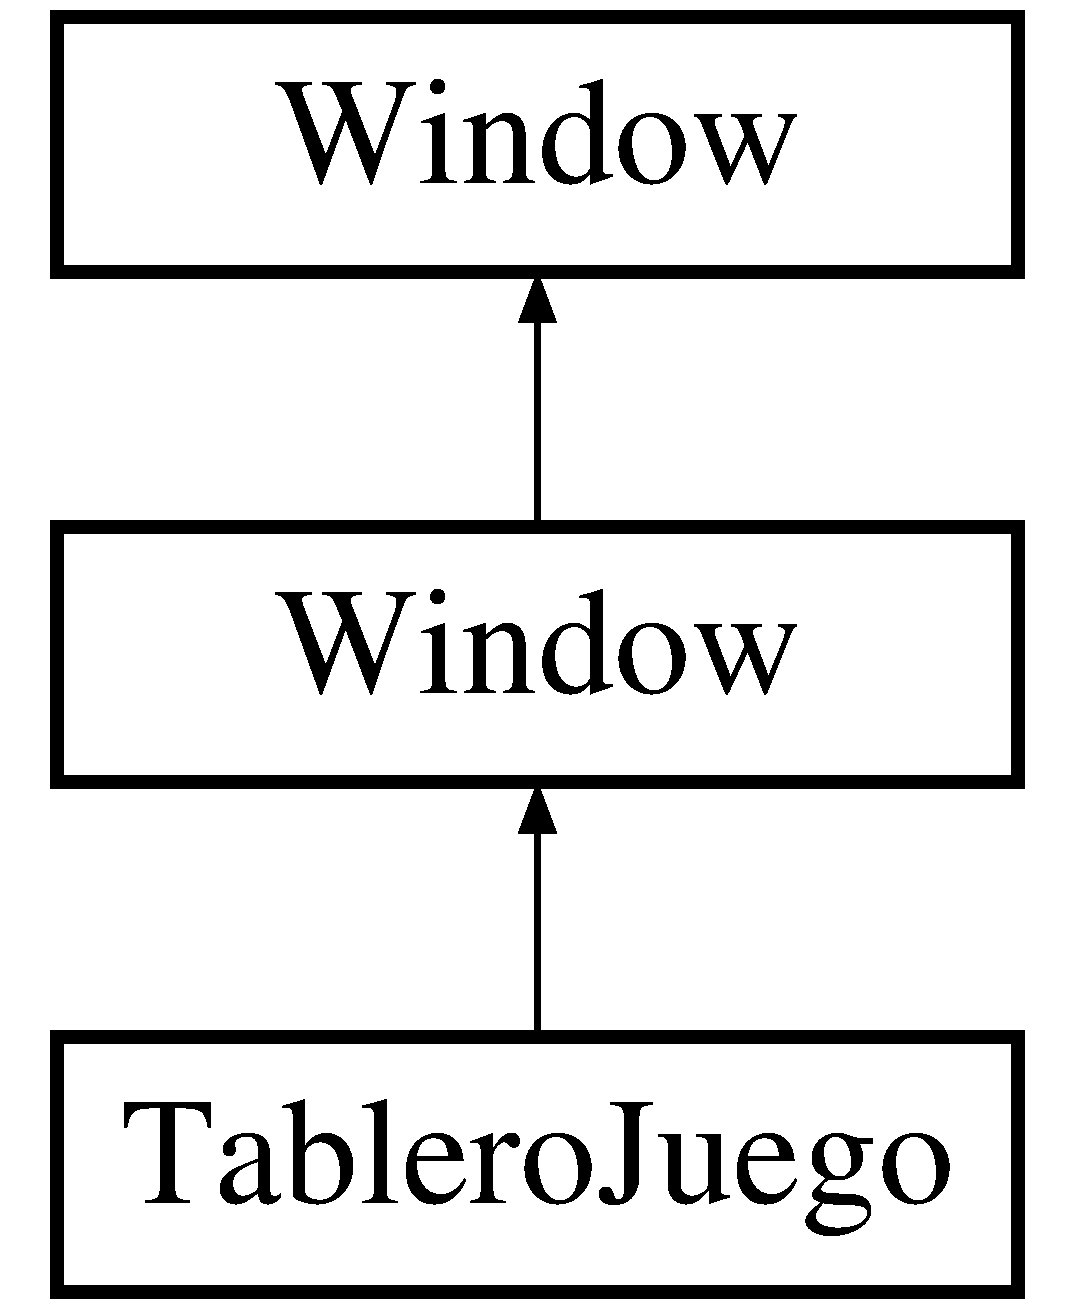
\includegraphics[height=3.000000cm]{classTableroJuego}
\end{center}
\end{figure}
\subsection*{Public Member Functions}
\begin{DoxyCompactItemize}
\item 
\hypertarget{classTableroJuego_a2eec33d7937d0456864c4f60974ba2eb}{{\bfseries Tablero\-Juego} (Json\-::\-Value mapa)}\label{classTableroJuego_a2eec33d7937d0456864c4f60974ba2eb}

\item 
\hypertarget{classTableroJuego_a15fd7203a35010f6c6d380cd7eba91fe}{void {\bfseries dibujar} ()}\label{classTableroJuego_a15fd7203a35010f6c6d380cd7eba91fe}

\item 
virtual void \hyperlink{classTableroJuego_a7da547b04514c8af0a68e9bf069d147b}{mensaje} (Json\-::\-Value \&data)
\end{DoxyCompactItemize}
\subsection*{Additional Inherited Members}


\subsection{Member Function Documentation}
\hypertarget{classTableroJuego_a7da547b04514c8af0a68e9bf069d147b}{\index{Tablero\-Juego@{Tablero\-Juego}!mensaje@{mensaje}}
\index{mensaje@{mensaje}!TableroJuego@{Tablero\-Juego}}
\subsubsection[{mensaje}]{\setlength{\rightskip}{0pt plus 5cm}void Tablero\-Juego\-::mensaje (
\begin{DoxyParamCaption}
\item[{Json\-::\-Value \&}]{data}
\end{DoxyParamCaption}
)\hspace{0.3cm}{\ttfamily [virtual]}}}\label{classTableroJuego_a7da547b04514c8af0a68e9bf069d147b}
Metodo que se usa para recibir mensajes. 
\begin{DoxyParams}{Parameters}
{\em data,\-:} & mensaje \{ \char`\"{}event\char`\"{}\-: , ... \} \\
\hline
\end{DoxyParams}


Implements \hyperlink{classWindow_a6034ea4f54b6647de07b19ff95fb22ae}{Window}.



The documentation for this class was generated from the following files\-:\begin{DoxyCompactItemize}
\item 
cliente.\-tablerojuego.\-h\item 
cliente.\-tablerojuego.\-cpp\end{DoxyCompactItemize}

\hypertarget{classTCPSocket}{\section{T\-C\-P\-Socket Class Reference}
\label{classTCPSocket}\index{T\-C\-P\-Socket@{T\-C\-P\-Socket}}
}
Inheritance diagram for T\-C\-P\-Socket\-:\begin{figure}[H]
\begin{center}
\leavevmode
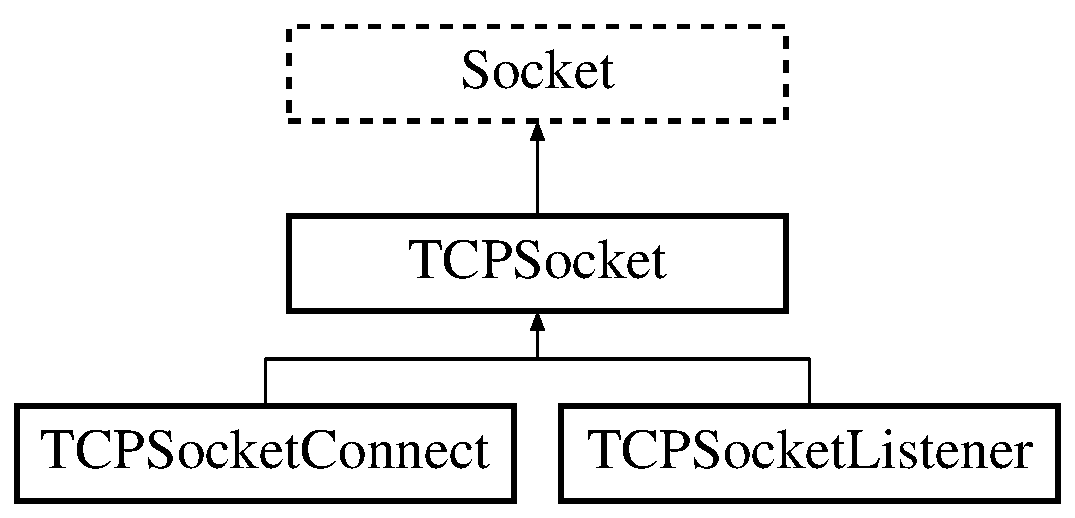
\includegraphics[height=3.000000cm]{classTCPSocket}
\end{center}
\end{figure}
\subsection*{Additional Inherited Members}


The documentation for this class was generated from the following files\-:\begin{DoxyCompactItemize}
\item 
common.\-socket.\-h\item 
common.\-socket.\-cpp\end{DoxyCompactItemize}

\hypertarget{classTCPSocketConnect}{\section{T\-C\-P\-Socket\-Connect Class Reference}
\label{classTCPSocketConnect}\index{T\-C\-P\-Socket\-Connect@{T\-C\-P\-Socket\-Connect}}
}


{\ttfamily \#include $<$cliente.\-socket\-\_\-connect.\-h$>$}

Inheritance diagram for T\-C\-P\-Socket\-Connect\-:\begin{figure}[H]
\begin{center}
\leavevmode
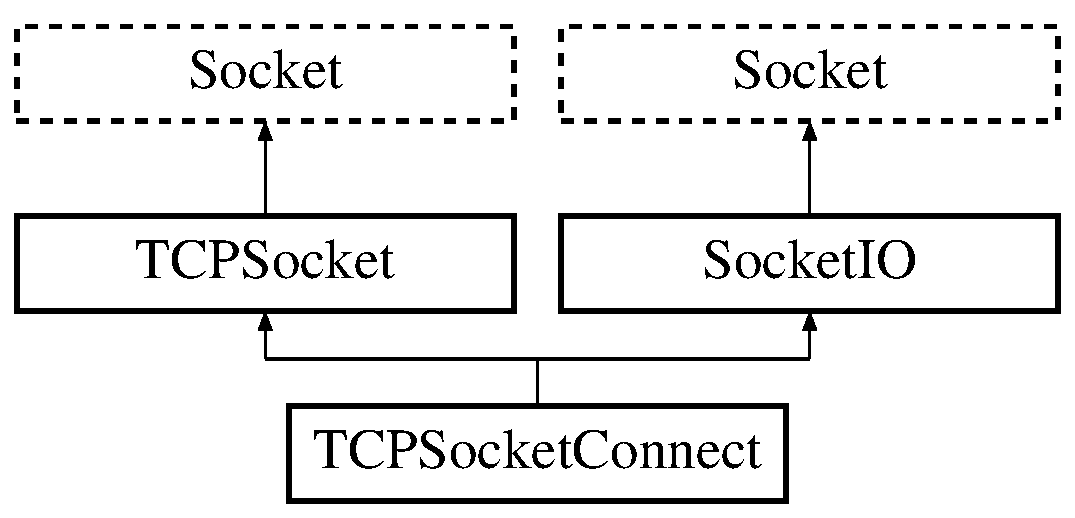
\includegraphics[height=3.000000cm]{classTCPSocketConnect}
\end{center}
\end{figure}
\subsection*{Public Member Functions}
\begin{DoxyCompactItemize}
\item 
\hypertarget{classTCPSocketConnect_a592be26bf68b59f04a91217b87b62b9c}{int {\bfseries connect} (const std\-::string \&ip)}\label{classTCPSocketConnect_a592be26bf68b59f04a91217b87b62b9c}

\item 
\hypertarget{classTCPSocketConnect_aa8bd820d4b7924dd2f556e8fb79c6ddd}{int {\bfseries connect} (const int port, const std\-::string \&ip)}\label{classTCPSocketConnect_aa8bd820d4b7924dd2f556e8fb79c6ddd}

\item 
\hypertarget{classTCPSocketConnect_ad2c5596b70e1278d0a5835b410d3e6f1}{int {\bfseries connect} (struct sockaddr\-\_\-in \&serv\-\_\-addr)}\label{classTCPSocketConnect_ad2c5596b70e1278d0a5835b410d3e6f1}

\end{DoxyCompactItemize}
\subsection*{Additional Inherited Members}


\subsection{Detailed Description}
\hyperlink{classSocket}{Socket} T\-C\-P que permite hacer una coneccion. 

The documentation for this class was generated from the following files\-:\begin{DoxyCompactItemize}
\item 
cliente.\-socket\-\_\-connect.\-h\item 
cliente.\-socket\-\_\-connect.\-cpp\end{DoxyCompactItemize}

\hypertarget{classTCPSocketListener}{\section{T\-C\-P\-Socket\-Listener Class Reference}
\label{classTCPSocketListener}\index{T\-C\-P\-Socket\-Listener@{T\-C\-P\-Socket\-Listener}}
}
Inheritance diagram for T\-C\-P\-Socket\-Listener\-:\begin{figure}[H]
\begin{center}
\leavevmode
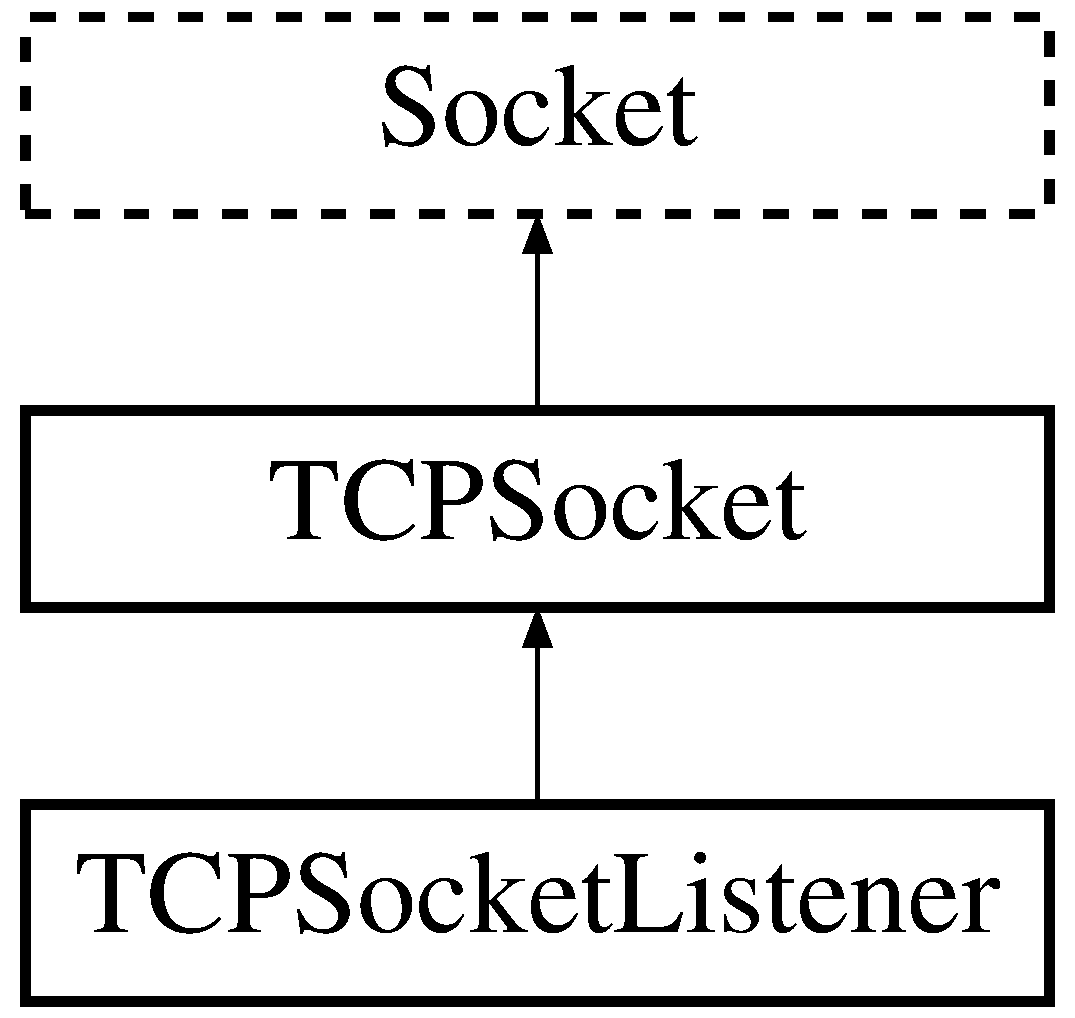
\includegraphics[height=3.000000cm]{classTCPSocketListener}
\end{center}
\end{figure}
\subsection*{Public Member Functions}
\begin{DoxyCompactItemize}
\item 
int \hyperlink{classTCPSocketListener_ac0f2aae9fd85f916c6d9cd05f4bfd7ef}{listen} (const int port)
\item 
\hypertarget{classTCPSocketListener_a693cccd1b9f304f746d8780d33248875}{int {\bfseries listen} (const int port, const std\-::string \&ip)}\label{classTCPSocketListener_a693cccd1b9f304f746d8780d33248875}

\item 
\hypertarget{classTCPSocketListener_af8455db0b7c454b3ba0b4ac2d4b9cd1c}{int {\bfseries listen} (struct sockaddr\-\_\-in \&serv\-\_\-addr)}\label{classTCPSocketListener_af8455db0b7c454b3ba0b4ac2d4b9cd1c}

\item 
\hyperlink{classSocketIO}{Socket\-I\-O} $\ast$ \hyperlink{classTCPSocketListener_a4cff944e470d8ef76807bceb3b6ce349}{accept} ()
\item 
\hypertarget{classTCPSocketListener_a7f098a2870d74ce9c87a774e1caaac77}{\hyperlink{classTCPSocketListener}{T\-C\-P\-Socket\-Listener} \& {\bfseries set\-Backlog} (const unsigned int backlog)}\label{classTCPSocketListener_a7f098a2870d74ce9c87a774e1caaac77}

\end{DoxyCompactItemize}
\subsection*{Protected Attributes}
\begin{DoxyCompactItemize}
\item 
\hypertarget{classTCPSocketListener_a1a166893f50a3668450bb155cfe24654}{unsigned int {\bfseries backlog}}\label{classTCPSocketListener_a1a166893f50a3668450bb155cfe24654}

\end{DoxyCompactItemize}
\subsection*{Additional Inherited Members}


\subsection{Member Function Documentation}
\hypertarget{classTCPSocketListener_a4cff944e470d8ef76807bceb3b6ce349}{\index{T\-C\-P\-Socket\-Listener@{T\-C\-P\-Socket\-Listener}!accept@{accept}}
\index{accept@{accept}!TCPSocketListener@{T\-C\-P\-Socket\-Listener}}
\subsubsection[{accept}]{\setlength{\rightskip}{0pt plus 5cm}{\bf Socket\-I\-O} $\ast$ T\-C\-P\-Socket\-Listener\-::accept (
\begin{DoxyParamCaption}
{}
\end{DoxyParamCaption}
)}}\label{classTCPSocketListener_a4cff944e470d8ef76807bceb3b6ce349}
Acepta una nueva conexion, devuelve un file descriptor. Bloqueante \hypertarget{classTCPSocketListener_ac0f2aae9fd85f916c6d9cd05f4bfd7ef}{\index{T\-C\-P\-Socket\-Listener@{T\-C\-P\-Socket\-Listener}!listen@{listen}}
\index{listen@{listen}!TCPSocketListener@{T\-C\-P\-Socket\-Listener}}
\subsubsection[{listen}]{\setlength{\rightskip}{0pt plus 5cm}int T\-C\-P\-Socket\-Listener\-::listen (
\begin{DoxyParamCaption}
\item[{const int}]{port}
\end{DoxyParamCaption}
)}}\label{classTCPSocketListener_ac0f2aae9fd85f916c6d9cd05f4bfd7ef}
Escucha a una nueva conexion. 

The documentation for this class was generated from the following files\-:\begin{DoxyCompactItemize}
\item 
server.\-socket\-\_\-listener.\-h\item 
server.\-socket\-\_\-listener.\-cpp\end{DoxyCompactItemize}

\hypertarget{classThread}{\section{Thread Class Reference}
\label{classThread}\index{Thread@{Thread}}
}
Inheritance diagram for Thread\-:\begin{figure}[H]
\begin{center}
\leavevmode
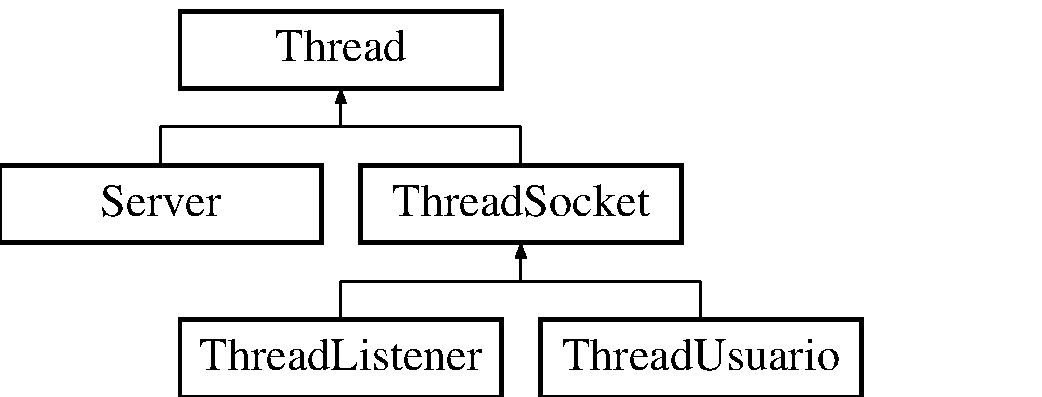
\includegraphics[height=3.000000cm]{classThread}
\end{center}
\end{figure}
\subsection*{Public Member Functions}
\begin{DoxyCompactItemize}
\item 
\hypertarget{classThread_a7d563f3201d081af8cc24ea552c6a4e4}{int {\bfseries start} ()}\label{classThread_a7d563f3201d081af8cc24ea552c6a4e4}

\item 
\hypertarget{classThread_a7c3b04b32b4327923cc4c9553a403e32}{int {\bfseries join} ()}\label{classThread_a7c3b04b32b4327923cc4c9553a403e32}

\item 
\hypertarget{classThread_a2a08036a4598cfc554114fee9d0e8485}{int {\bfseries detach} ()}\label{classThread_a2a08036a4598cfc554114fee9d0e8485}

\end{DoxyCompactItemize}
\subsection*{Protected Member Functions}
\begin{DoxyCompactItemize}
\item 
\hypertarget{classThread_a0ceaa28981eacf1051845542053d82b6}{virtual void $\ast$ {\bfseries run} ()=0}\label{classThread_a0ceaa28981eacf1051845542053d82b6}

\end{DoxyCompactItemize}


The documentation for this class was generated from the following files\-:\begin{DoxyCompactItemize}
\item 
common.\-thread.\-h\item 
common.\-thread.\-cpp\end{DoxyCompactItemize}

\hypertarget{classThreadListener}{\section{Thread\-Listener Class Reference}
\label{classThreadListener}\index{Thread\-Listener@{Thread\-Listener}}
}


{\ttfamily \#include $<$cliente.\-thread\-\_\-listener.\-h$>$}

Inheritance diagram for Thread\-Listener\-:\begin{figure}[H]
\begin{center}
\leavevmode
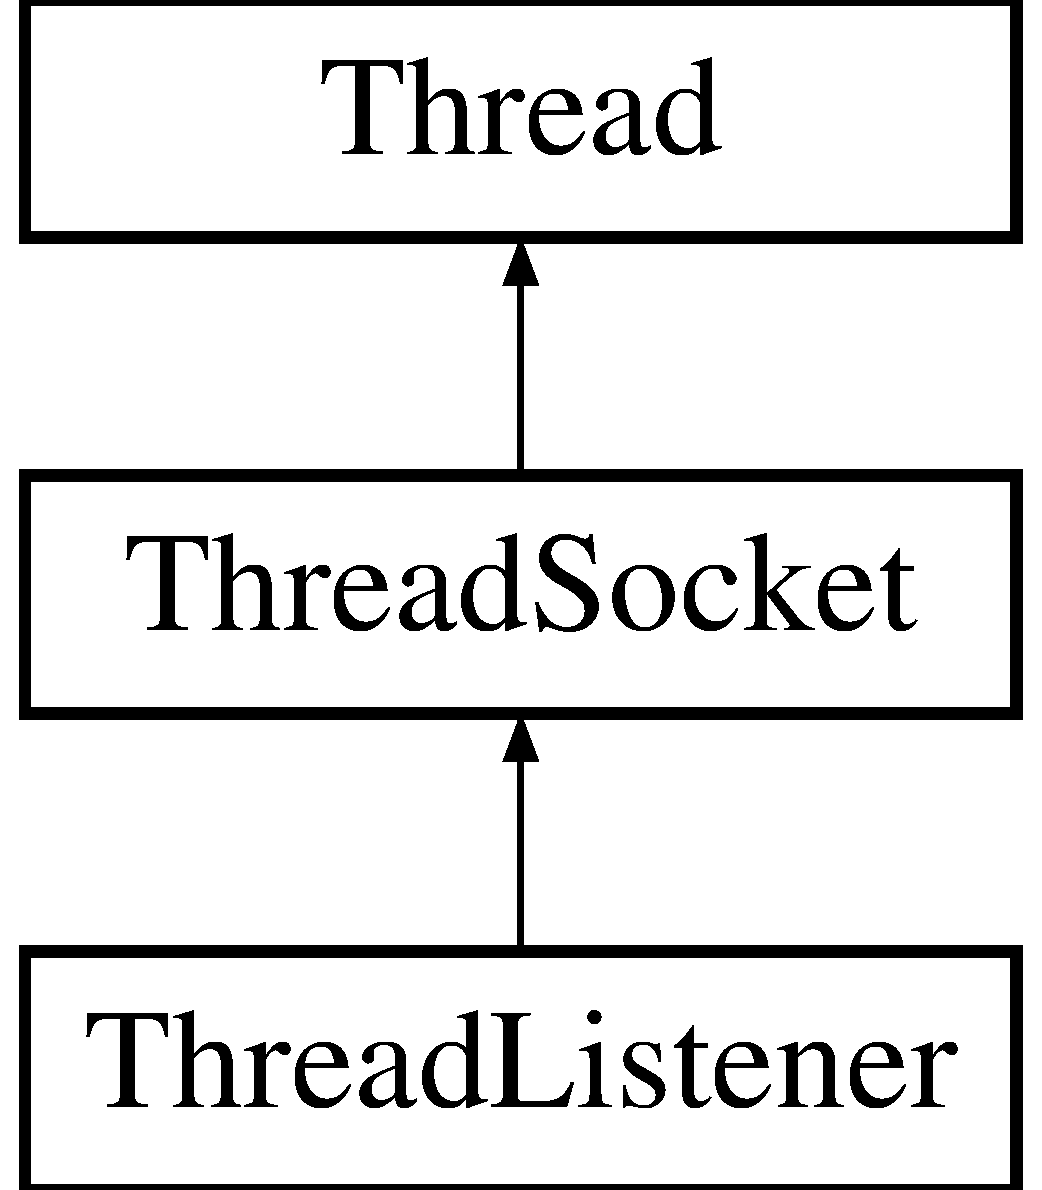
\includegraphics[height=3.000000cm]{classThreadListener}
\end{center}
\end{figure}
\subsection*{Public Member Functions}
\begin{DoxyCompactItemize}
\item 
\hypertarget{classThreadListener_a2b74bbe948a95248dfc86dda0d597b45}{{\bfseries Thread\-Listener} (\hyperlink{classClienteInterface}{Cliente\-Interface} $\ast$s, \hyperlink{classSocketIO}{Socket\-I\-O} $\ast$fd)}\label{classThreadListener_a2b74bbe948a95248dfc86dda0d597b45}

\item 
void \hyperlink{classThreadListener_a8fb16a6bf5b346c368cf4a190699eefc}{set\-Key} (std\-::string \&key)
\end{DoxyCompactItemize}
\subsection*{Protected Member Functions}
\begin{DoxyCompactItemize}
\item 
\hypertarget{classThreadListener_a76186eca6fa62382baf0a7835abe3668}{virtual int {\bfseries event\-No\-Firmado} (Json\-::\-Value \&data)}\label{classThreadListener_a76186eca6fa62382baf0a7835abe3668}

\item 
\hypertarget{classThreadListener_a510060ad5fbaa44711574b409b4ccaa8}{virtual int {\bfseries event\-Firmado} (Json\-::\-Value \&data)}\label{classThreadListener_a510060ad5fbaa44711574b409b4ccaa8}

\item 
\hypertarget{classThreadListener_aacfdbbcb7b2f30a7e757e6c4cde14657}{virtual void $\ast$ {\bfseries sub\-Run} ()}\label{classThreadListener_aacfdbbcb7b2f30a7e757e6c4cde14657}

\end{DoxyCompactItemize}
\subsection*{Protected Attributes}
\begin{DoxyCompactItemize}
\item 
\hypertarget{classThreadListener_a9d1782a3bd19b633935c29b8c45d2e27}{\hyperlink{classClienteInterface}{Cliente\-Interface} $\ast$ {\bfseries cliente}}\label{classThreadListener_a9d1782a3bd19b633935c29b8c45d2e27}

\end{DoxyCompactItemize}


\subsection{Detailed Description}
\hyperlink{classThread}{Thread} que se encarga de leer constantemente al socket. De recibir algun mensaje lo agrega a la cola de mensajes del cliente. 

\subsection{Member Function Documentation}
\hypertarget{classThreadListener_a8fb16a6bf5b346c368cf4a190699eefc}{\index{Thread\-Listener@{Thread\-Listener}!set\-Key@{set\-Key}}
\index{set\-Key@{set\-Key}!ThreadListener@{Thread\-Listener}}
\subsubsection[{set\-Key}]{\setlength{\rightskip}{0pt plus 5cm}void Thread\-Listener\-::set\-Key (
\begin{DoxyParamCaption}
\item[{std\-::string \&}]{key}
\end{DoxyParamCaption}
)}}\label{classThreadListener_a8fb16a6bf5b346c368cf4a190699eefc}
Setear la clave usada para la firma digital de los paquetes 

The documentation for this class was generated from the following files\-:\begin{DoxyCompactItemize}
\item 
cliente.\-thread\-\_\-listener.\-h\item 
cliente.\-thread\-\_\-listener.\-cpp\end{DoxyCompactItemize}

\hypertarget{classThreadSocket}{\section{Thread\-Socket Class Reference}
\label{classThreadSocket}\index{Thread\-Socket@{Thread\-Socket}}
}


{\ttfamily \#include $<$common.\-thread\-\_\-socket.\-h$>$}

Inheritance diagram for Thread\-Socket\-:\begin{figure}[H]
\begin{center}
\leavevmode
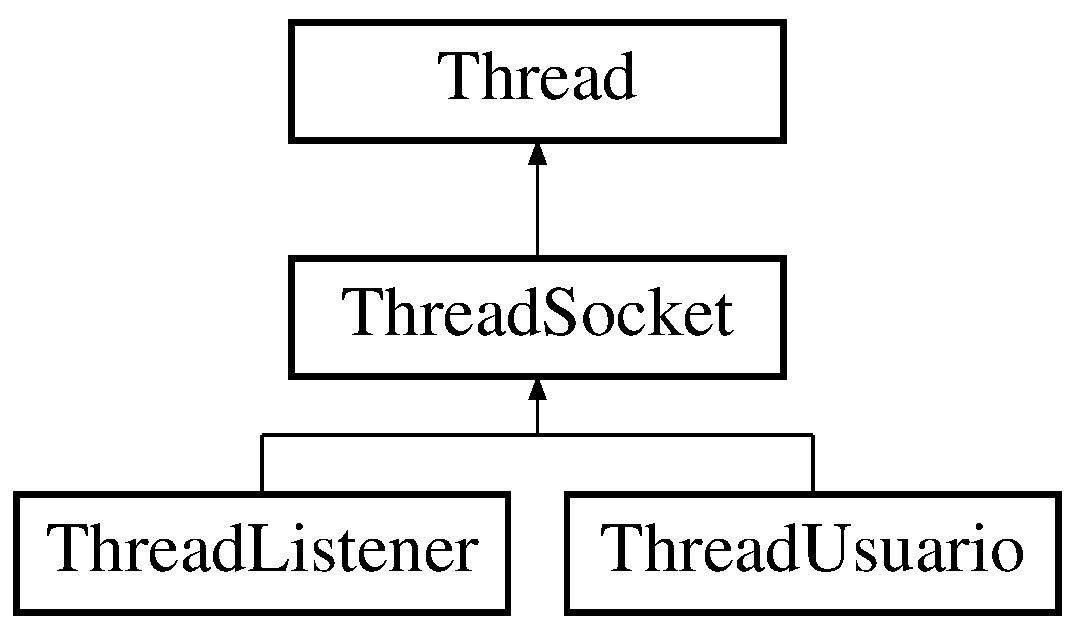
\includegraphics[height=3.000000cm]{classThreadSocket}
\end{center}
\end{figure}
\subsection*{Public Member Functions}
\begin{DoxyCompactItemize}
\item 
\hypertarget{classThreadSocket_acde9e8d6f617c737b3f1fcae8dbd5035}{{\bfseries Thread\-Socket} (\hyperlink{classSocketIO}{Socket\-I\-O} $\ast$fd)}\label{classThreadSocket_acde9e8d6f617c737b3f1fcae8dbd5035}

\item 
\hypertarget{classThreadSocket_adcd69d1774f9446524447212dc1aa4cf}{int {\bfseries shutdown} (int how)}\label{classThreadSocket_adcd69d1774f9446524447212dc1aa4cf}

\item 
\hypertarget{classThreadSocket_ad449f071be16b20b3a224602fc0cc1ac}{int {\bfseries shutdown} ()}\label{classThreadSocket_ad449f071be16b20b3a224602fc0cc1ac}

\item 
\hypertarget{classThreadSocket_a8c818be3e8fd7318494766e06346a58e}{int {\bfseries write} (Json\-::\-Value data)}\label{classThreadSocket_a8c818be3e8fd7318494766e06346a58e}

\end{DoxyCompactItemize}
\subsection*{Protected Member Functions}
\begin{DoxyCompactItemize}
\item 
\hypertarget{classThreadSocket_af1b0cef0db707285a0b85859604c9108}{virtual void $\ast$ {\bfseries run} ()}\label{classThreadSocket_af1b0cef0db707285a0b85859604c9108}

\item 
\hypertarget{classThreadSocket_a7053b41c6b371af8196846f4a8fb4efd}{virtual void $\ast$ {\bfseries sub\-Run} ()=0}\label{classThreadSocket_a7053b41c6b371af8196846f4a8fb4efd}

\item 
\hypertarget{classThreadSocket_a10bcf11e1b8ee011517598ebc6743a0f}{int {\bfseries read} (bool check=true)}\label{classThreadSocket_a10bcf11e1b8ee011517598ebc6743a0f}

\item 
\hypertarget{classThreadSocket_a06335dda20d235a6a39c2996bff43187}{virtual int {\bfseries event\-No\-Firmado} (Json\-::\-Value \&data)=0}\label{classThreadSocket_a06335dda20d235a6a39c2996bff43187}

\item 
\hypertarget{classThreadSocket_a91d3707cd81604c3667813bdcdee19fb}{virtual int {\bfseries event\-Firmado} (Json\-::\-Value \&data)=0}\label{classThreadSocket_a91d3707cd81604c3667813bdcdee19fb}

\end{DoxyCompactItemize}
\subsection*{Protected Attributes}
\begin{DoxyCompactItemize}
\item 
\hypertarget{classThreadSocket_ad04462842b9d43917bf42f19949f0396}{\hyperlink{classSocketIO}{Socket\-I\-O} $\ast$ {\bfseries fd}}\label{classThreadSocket_ad04462842b9d43917bf42f19949f0396}

\item 
\hypertarget{classThreadSocket_a1d262d599d927682b104c667d7da2b4a}{\hyperlink{classMutex}{Mutex} {\bfseries write\-Mutex}}\label{classThreadSocket_a1d262d599d927682b104c667d7da2b4a}

\item 
\hypertarget{classThreadSocket_aad2ecc5af11bbf135d5bcf85bc717fd9}{std\-::string {\bfseries my\-Id}}\label{classThreadSocket_aad2ecc5af11bbf135d5bcf85bc717fd9}

\item 
\hypertarget{classThreadSocket_a48d57199861265eec3eeb69eacd92198}{std\-::string {\bfseries key}}\label{classThreadSocket_a48d57199861265eec3eeb69eacd92198}

\end{DoxyCompactItemize}


\subsection{Detailed Description}
\hyperlink{classThread}{Thread} encargado del manejo de un socket. Posee un metodo de escritura protegida con mutex, la lectura siempre se hace dentro del thread. 

The documentation for this class was generated from the following files\-:\begin{DoxyCompactItemize}
\item 
common.\-thread\-\_\-socket.\-h\item 
common.\-thread\-\_\-socket.\-cpp\end{DoxyCompactItemize}

\hypertarget{classThreadUsuario}{\section{Thread\-Usuario Class Reference}
\label{classThreadUsuario}\index{Thread\-Usuario@{Thread\-Usuario}}
}


{\ttfamily \#include $<$server.\-thread\-\_\-usuario.\-h$>$}

Inheritance diagram for Thread\-Usuario\-:\begin{figure}[H]
\begin{center}
\leavevmode
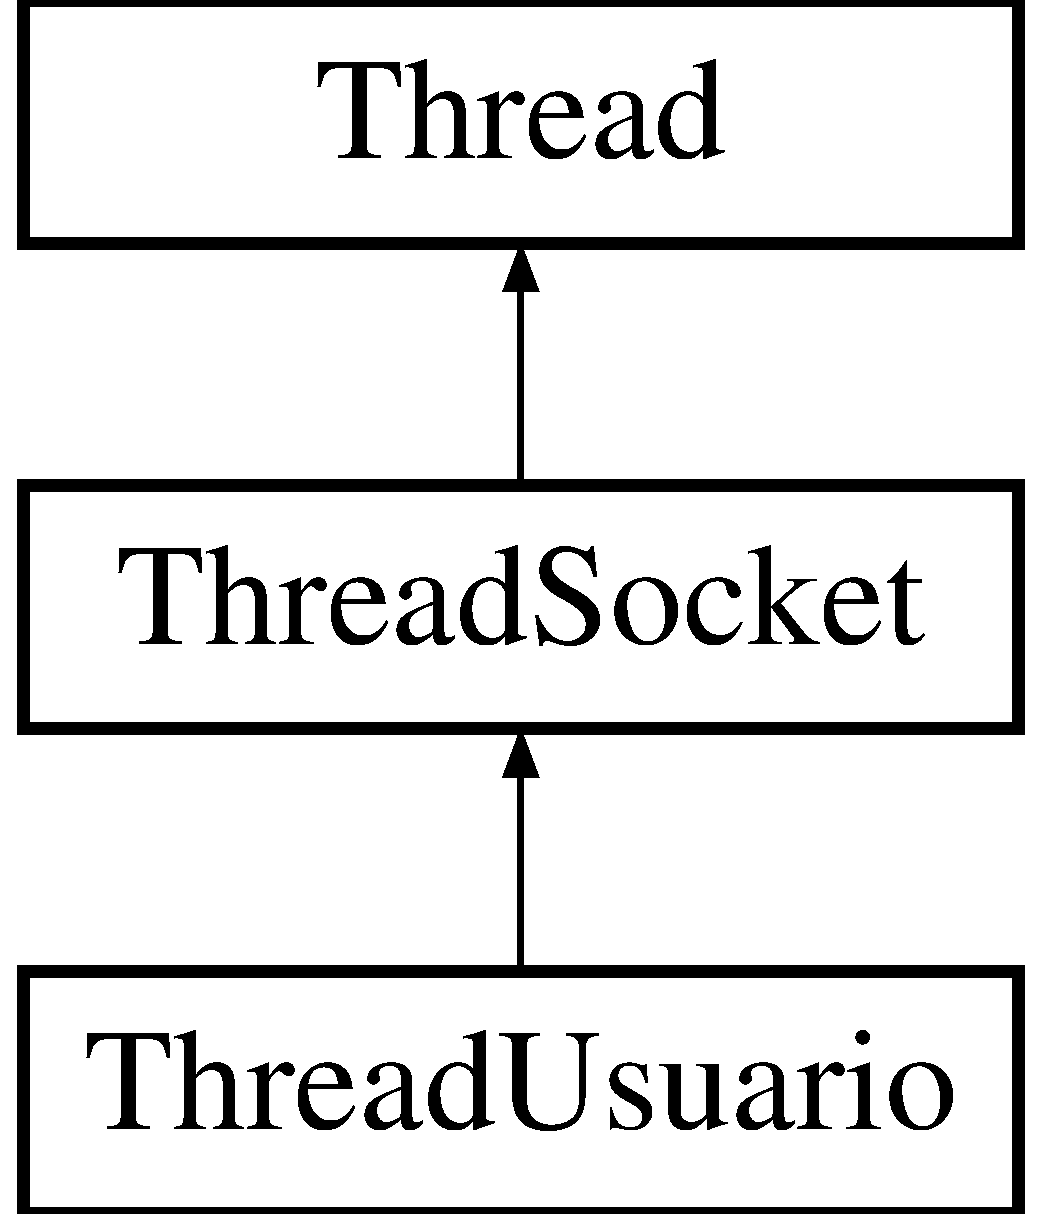
\includegraphics[height=3.000000cm]{classThreadUsuario}
\end{center}
\end{figure}
\subsection*{Public Member Functions}
\begin{DoxyCompactItemize}
\item 
\hypertarget{classThreadUsuario_a89614bb5871f99c8effaba450e5aa4f0}{{\bfseries Thread\-Usuario} (\hyperlink{classServerInterface}{Server\-Interface} $\ast$s, \hyperlink{classSocketIO}{Socket\-I\-O} $\ast$fd)}\label{classThreadUsuario_a89614bb5871f99c8effaba450e5aa4f0}

\end{DoxyCompactItemize}
\subsection*{Protected Member Functions}
\begin{DoxyCompactItemize}
\item 
\hypertarget{classThreadUsuario_a8e1776d0b712b02710564f5172476fab}{virtual int {\bfseries event\-No\-Firmado} (Json\-::\-Value \&data)}\label{classThreadUsuario_a8e1776d0b712b02710564f5172476fab}

\item 
\hypertarget{classThreadUsuario_a0ed65fc90c1e188cd3a492dbebf9d0a2}{virtual int {\bfseries event\-Firmado} (Json\-::\-Value \&data)}\label{classThreadUsuario_a0ed65fc90c1e188cd3a492dbebf9d0a2}

\item 
\hypertarget{classThreadUsuario_a7f7c0738bd4320e3f9f2eb065a2d45f3}{virtual void $\ast$ {\bfseries sub\-Run} ()}\label{classThreadUsuario_a7f7c0738bd4320e3f9f2eb065a2d45f3}

\item 
\hypertarget{classThreadUsuario_ab51cc252bc76f33fefb4b601f47b289c}{int {\bfseries on\-Join\-Game} (Json\-::\-Value \&data, Json\-::\-Value \&user\-Data)}\label{classThreadUsuario_ab51cc252bc76f33fefb4b601f47b289c}

\item 
\hypertarget{classThreadUsuario_a541854eb8f6a5c47cec0ebc30e403bc8}{int {\bfseries on\-Leave\-Game} (Json\-::\-Value \&data, Json\-::\-Value \&user\-Data)}\label{classThreadUsuario_a541854eb8f6a5c47cec0ebc30e403bc8}

\item 
\hypertarget{classThreadUsuario_ab6033809c7c416bb2210c7fabec26ae7}{int {\bfseries on\-New\-Game} (Json\-::\-Value \&data, Json\-::\-Value \&user\-Data)}\label{classThreadUsuario_ab6033809c7c416bb2210c7fabec26ae7}

\item 
\hypertarget{classThreadUsuario_a56b98549728c0f4aa77282325414ca32}{int {\bfseries on\-Get\-Maps} (Json\-::\-Value \&data, Json\-::\-Value \&user\-Data)}\label{classThreadUsuario_a56b98549728c0f4aa77282325414ca32}

\item 
\hypertarget{classThreadUsuario_a88100073941ca7caf1a38dd019e10946}{int {\bfseries welcome} ()}\label{classThreadUsuario_a88100073941ca7caf1a38dd019e10946}

\end{DoxyCompactItemize}
\subsection*{Protected Attributes}
\begin{DoxyCompactItemize}
\item 
\hypertarget{classThreadUsuario_ab778e6d6893a51191a76cc4a7f45938b}{\hyperlink{classServerInterface}{Server\-Interface} $\ast$ {\bfseries server}}\label{classThreadUsuario_ab778e6d6893a51191a76cc4a7f45938b}

\item 
\hypertarget{classThreadUsuario_a161d5b28cdbd8116969bf698ebec11c3}{\hyperlink{classPartidaInterface}{Partida\-Interface} $\ast$ {\bfseries partida}}\label{classThreadUsuario_a161d5b28cdbd8116969bf698ebec11c3}

\item 
\hypertarget{classThreadUsuario_a513f404350b08bee0b09b0291869a660}{std\-::string {\bfseries user}}\label{classThreadUsuario_a513f404350b08bee0b09b0291869a660}

\end{DoxyCompactItemize}


\subsection{Detailed Description}
\hyperlink{classThread}{Thread} usado para cada usuario que se conecta 

The documentation for this class was generated from the following files\-:\begin{DoxyCompactItemize}
\item 
server.\-thread\-\_\-usuario.\-h\item 
server.\-thread\-\_\-usuario.\-cpp\end{DoxyCompactItemize}

\hypertarget{structTWavArgs}{\section{T\-Wav\-Args Struct Reference}
\label{structTWavArgs}\index{T\-Wav\-Args@{T\-Wav\-Args}}
}
\subsection*{Public Attributes}
\begin{DoxyCompactItemize}
\item 
\hypertarget{structTWavArgs_a531620488d50622828137833592ab8d9}{int {\bfseries sample\-\_\-rate}}\label{structTWavArgs_a531620488d50622828137833592ab8d9}

\item 
\hypertarget{structTWavArgs_a84d83e5cdbd062fb51849f07cdb08fbb}{int {\bfseries channels}}\label{structTWavArgs_a84d83e5cdbd062fb51849f07cdb08fbb}

\item 
\hypertarget{structTWavArgs_a8cd4a5f5b1a07dd824aaf8cf42e775db}{int {\bfseries seconds}}\label{structTWavArgs_a8cd4a5f5b1a07dd824aaf8cf42e775db}

\item 
\hypertarget{structTWavArgs_a770ba7334153112aa7fd588b3597765e}{int {\bfseries fd}}\label{structTWavArgs_a770ba7334153112aa7fd588b3597765e}

\end{DoxyCompactItemize}


The documentation for this struct was generated from the following file\-:\begin{DoxyCompactItemize}
\item 
cliente.\-sound\-\_\-player.\-cpp\end{DoxyCompactItemize}

\hypertarget{structTWavHeader}{\section{T\-Wav\-Header Struct Reference}
\label{structTWavHeader}\index{T\-Wav\-Header@{T\-Wav\-Header}}
}
\subsection*{Public Attributes}
\begin{DoxyCompactItemize}
\item 
\hypertarget{structTWavHeader_a8f7cef0ea47060bc2c39215d65190cf0}{char {\bfseries riff} \mbox{[}4\mbox{]}}\label{structTWavHeader_a8f7cef0ea47060bc2c39215d65190cf0}

\item 
\hypertarget{structTWavHeader_ab7a5d66f1d330dcaeec23fbac8e5170c}{uint32\-\_\-t {\bfseries size}}\label{structTWavHeader_ab7a5d66f1d330dcaeec23fbac8e5170c}

\item 
\hypertarget{structTWavHeader_a78a648bed553acac2435561542c547c3}{char {\bfseries wave} \mbox{[}4\mbox{]}}\label{structTWavHeader_a78a648bed553acac2435561542c547c3}

\item 
\hypertarget{structTWavHeader_ae618233b087bf9af4d51d1877857ceac}{uint16\-\_\-t {\bfseries fmt}}\label{structTWavHeader_ae618233b087bf9af4d51d1877857ceac}

\item 
\hypertarget{structTWavHeader_a2934af23aeee8dd8612f380cffb93f5c}{uint32\-\_\-t {\bfseries length}}\label{structTWavHeader_a2934af23aeee8dd8612f380cffb93f5c}

\item 
\hypertarget{structTWavHeader_a91b2a0acae0e0bb3040b741521addc44}{uint16\-\_\-t {\bfseries type}}\label{structTWavHeader_a91b2a0acae0e0bb3040b741521addc44}

\item 
\hypertarget{structTWavHeader_a8e5a38b7cc4aeb25e71a3ad83e5c820a}{uint16\-\_\-t {\bfseries channels}}\label{structTWavHeader_a8e5a38b7cc4aeb25e71a3ad83e5c820a}

\item 
\hypertarget{structTWavHeader_ac81c6f1ee53a8b1dfeb58b7628f5956f}{uint32\-\_\-t {\bfseries sample\-\_\-rate}}\label{structTWavHeader_ac81c6f1ee53a8b1dfeb58b7628f5956f}

\item 
\hypertarget{structTWavHeader_a2470e86e5258bd285262323a3ab96771}{uint32\-\_\-t {\bfseries bit\-\_\-rate}}\label{structTWavHeader_a2470e86e5258bd285262323a3ab96771}

\item 
\hypertarget{structTWavHeader_aa463a443f52fb3f2cc2f249ddf046063}{uint32\-\_\-t {\bfseries bits\-\_\-per\-\_\-sample}}\label{structTWavHeader_aa463a443f52fb3f2cc2f249ddf046063}

\item 
\hypertarget{structTWavHeader_adce8403001ab3f9e0e8c9b133b81e054}{char {\bfseries data} \mbox{[}4\mbox{]}}\label{structTWavHeader_adce8403001ab3f9e0e8c9b133b81e054}

\item 
\hypertarget{structTWavHeader_a72fbdd2ccca8b4d729b404e280a31684}{uint32\-\_\-t {\bfseries file\-\_\-size}}\label{structTWavHeader_a72fbdd2ccca8b4d729b404e280a31684}

\end{DoxyCompactItemize}


The documentation for this struct was generated from the following file\-:\begin{DoxyCompactItemize}
\item 
cliente.\-sound\-\_\-player.\-cpp\end{DoxyCompactItemize}

\hypertarget{classUserManager}{\section{User\-Manager Class Reference}
\label{classUserManager}\index{User\-Manager@{User\-Manager}}
}


{\ttfamily \#include $<$common.\-user\-\_\-manager.\-h$>$}

\subsection*{Static Public Member Functions}
\begin{DoxyCompactItemize}
\item 
\hypertarget{classUserManager_a712e64b638d4586652bca563c19f427c}{static void {\bfseries init} (const std\-::string \&path)}\label{classUserManager_a712e64b638d4586652bca563c19f427c}

\item 
\hypertarget{classUserManager_aacdfb7ae91fee25bf7d61f047299396f}{static void {\bfseries destroy} ()}\label{classUserManager_aacdfb7ae91fee25bf7d61f047299396f}

\item 
static void \hyperlink{classUserManager_a42d338740bb3317751799a3e85b15903}{get} (const std\-::string \&user, Json\-::\-Value \&data)
\item 
static int \hyperlink{classUserManager_a78eee9121e7ceb88c18ec011391bd397}{set} (const Json\-::\-Value \&data)
\end{DoxyCompactItemize}
\subsection*{Protected Member Functions}
\begin{DoxyCompactItemize}
\item 
\hypertarget{classUserManager_a450ad78085c4462f149023559d7876eb}{{\bfseries User\-Manager} (const std\-::string \&path)}\label{classUserManager_a450ad78085c4462f149023559d7876eb}

\item 
\hypertarget{classUserManager_aecad336ff52d5121e6bdd61636a91f45}{void {\bfseries \-\_\-get} (const std\-::string \&user, Json\-::\-Value \&data)}\label{classUserManager_aecad336ff52d5121e6bdd61636a91f45}

\item 
\hypertarget{classUserManager_a3160806deccfc95412a275696ff57074}{int {\bfseries \-\_\-set} (const Json\-::\-Value \&data)}\label{classUserManager_a3160806deccfc95412a275696ff57074}

\end{DoxyCompactItemize}
\subsection*{Protected Attributes}
\begin{DoxyCompactItemize}
\item 
\hypertarget{classUserManager_adcd1cf9ee71d16fbeadd6cb7c9a04656}{std\-::string {\bfseries path}}\label{classUserManager_adcd1cf9ee71d16fbeadd6cb7c9a04656}

\item 
\hypertarget{classUserManager_aa996769bd40f6d2d0c3a88cc3f69f422}{Json\-::\-Value {\bfseries users}}\label{classUserManager_aa996769bd40f6d2d0c3a88cc3f69f422}

\item 
\hypertarget{classUserManager_ae251a67890e92d82c4d6bc9b26cd6cfd}{\hyperlink{classMutex}{Mutex} {\bfseries mut}}\label{classUserManager_ae251a67890e92d82c4d6bc9b26cd6cfd}

\end{DoxyCompactItemize}
\subsection*{Static Protected Attributes}
\begin{DoxyCompactItemize}
\item 
\hypertarget{classUserManager_acae4ad483ab485ac3747da2a2f3f9e45}{static \hyperlink{classUserManager}{User\-Manager} $\ast$ {\bfseries me} = N\-U\-L\-L}\label{classUserManager_acae4ad483ab485ac3747da2a2f3f9e45}

\end{DoxyCompactItemize}


\subsection{Detailed Description}
Clase estilo singleton encargada del manejo de toda la informacion de los usuarios. Se la debe iniciar con init y destruir con destroy. 

\subsection{Member Function Documentation}
\hypertarget{classUserManager_a42d338740bb3317751799a3e85b15903}{\index{User\-Manager@{User\-Manager}!get@{get}}
\index{get@{get}!UserManager@{User\-Manager}}
\subsubsection[{get}]{\setlength{\rightskip}{0pt plus 5cm}void User\-Manager\-::get (
\begin{DoxyParamCaption}
\item[{const std\-::string \&}]{user, }
\item[{Json\-::\-Value \&}]{data}
\end{DoxyParamCaption}
)\hspace{0.3cm}{\ttfamily [static]}}}\label{classUserManager_a42d338740bb3317751799a3e85b15903}
Obtiene la informacion de un usario. 
\begin{DoxyParams}{Parameters}
{\em user\mbox{[}in\mbox{]},\-:} & nombre del usuario. \\
\hline
{\em data\mbox{[}out\mbox{]},\-:} & informacion del usuario \\
\hline
\end{DoxyParams}
\hypertarget{classUserManager_a78eee9121e7ceb88c18ec011391bd397}{\index{User\-Manager@{User\-Manager}!set@{set}}
\index{set@{set}!UserManager@{User\-Manager}}
\subsubsection[{set}]{\setlength{\rightskip}{0pt plus 5cm}int User\-Manager\-::set (
\begin{DoxyParamCaption}
\item[{const Json\-::\-Value \&}]{data}
\end{DoxyParamCaption}
)\hspace{0.3cm}{\ttfamily [static]}}}\label{classUserManager_a78eee9121e7ceb88c18ec011391bd397}
Setea y guarda la informacion (recordar que el nombre de usaurio esta dentro de la data. 
\begin{DoxyParams}{Parameters}
{\em data\mbox{[}in\mbox{]},\-:} & informacion del usuario \\
\hline
\end{DoxyParams}


The documentation for this class was generated from the following files\-:\begin{DoxyCompactItemize}
\item 
common.\-user\-\_\-manager.\-h\item 
common.\-user\-\_\-manager.\-cpp\end{DoxyCompactItemize}

\hypertarget{classWindow}{\section{Window Class Reference}
\label{classWindow}\index{Window@{Window}}
}


{\ttfamily \#include $<$cliente.\-window.\-h$>$}

Inheritance diagram for Window\-:\begin{figure}[H]
\begin{center}
\leavevmode
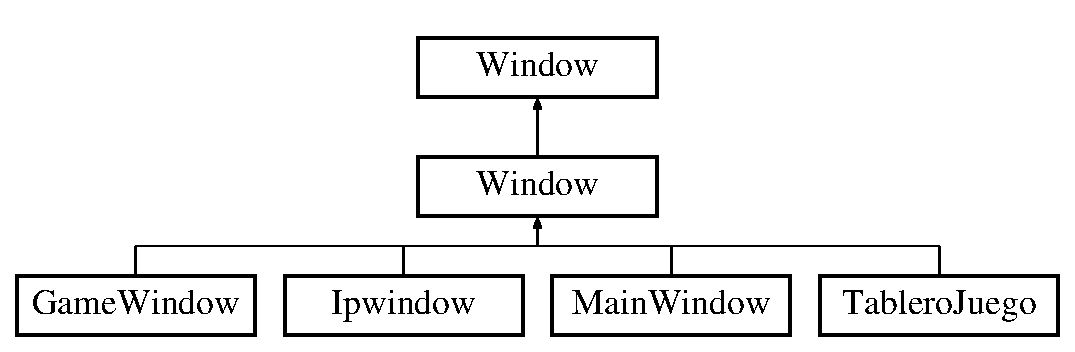
\includegraphics[height=3.000000cm]{classWindow}
\end{center}
\end{figure}
\subsection*{Public Types}
\begin{DoxyCompactItemize}
\item 
typedef sigc\-::signal$<$ void, \\*
Json\-::\-Value $>$ \hyperlink{classWindow_aee13a32f2064bb223c52ed10f8e41cb7}{type\-\_\-signal\-\_\-mensaje}
\end{DoxyCompactItemize}
\subsection*{Public Member Functions}
\begin{DoxyCompactItemize}
\item 
virtual void \hyperlink{classWindow_a6034ea4f54b6647de07b19ff95fb22ae}{mensaje} (Json\-::\-Value \&data)=0
\item 
\hypertarget{classWindow_a6d58f947e191a7c43d2578af1bae0bc5}{\hyperlink{classWindow_aee13a32f2064bb223c52ed10f8e41cb7}{type\-\_\-signal\-\_\-mensaje} {\bfseries signal\-\_\-mensaje} ()}\label{classWindow_a6d58f947e191a7c43d2578af1bae0bc5}

\item 
\hypertarget{classWindow_aa675d86b2857aac2a9111f8e8f473312}{void {\bfseries on\-\_\-about} ()}\label{classWindow_aa675d86b2857aac2a9111f8e8f473312}

\end{DoxyCompactItemize}
\subsection*{Protected Member Functions}
\begin{DoxyCompactItemize}
\item 
\hypertarget{classWindow_a8ad38ade5b5db7841a1ec0766e8aad75}{bool {\bfseries \-\_\-on\-Close} (Gdk\-Event\-Any $\ast$event)}\label{classWindow_a8ad38ade5b5db7841a1ec0766e8aad75}

\item 
\hypertarget{classWindow_a979cfd2bc52650f07b789217d6c6f570}{virtual bool {\bfseries on\-Close} ()}\label{classWindow_a979cfd2bc52650f07b789217d6c6f570}

\item 
\hypertarget{classWindow_a79dbd85218e5c2387b2d08f296304f50}{void {\bfseries set\-\_\-background\-\_\-image} (std\-::string path)}\label{classWindow_a79dbd85218e5c2387b2d08f296304f50}

\item 
\hypertarget{classWindow_a5837f14ab5bf0904be34909c440229ed}{bool {\bfseries dialog} (const char $\ast$pri, const char $\ast$sec)}\label{classWindow_a5837f14ab5bf0904be34909c440229ed}

\item 
\hypertarget{classWindow_a9891d6779c20eee09f911bbd53a5e45b}{bool {\bfseries dialog} (const std\-::string \&pri, const std\-::string \&sec)}\label{classWindow_a9891d6779c20eee09f911bbd53a5e45b}

\end{DoxyCompactItemize}
\subsection*{Protected Attributes}
\begin{DoxyCompactItemize}
\item 
\hypertarget{classWindow_a0a72d287d0625642dc3e704a61d16f88}{\hyperlink{classWindow_aee13a32f2064bb223c52ed10f8e41cb7}{type\-\_\-signal\-\_\-mensaje} {\bfseries m\-\_\-signal\-\_\-mensaje}}\label{classWindow_a0a72d287d0625642dc3e704a61d16f88}

\end{DoxyCompactItemize}


\subsection{Detailed Description}
Interfaz de ventana para todas las ventanas del cliente. 

\subsection{Member Typedef Documentation}
\hypertarget{classWindow_aee13a32f2064bb223c52ed10f8e41cb7}{\index{Window@{Window}!type\-\_\-signal\-\_\-mensaje@{type\-\_\-signal\-\_\-mensaje}}
\index{type\-\_\-signal\-\_\-mensaje@{type\-\_\-signal\-\_\-mensaje}!Window@{Window}}
\subsubsection[{type\-\_\-signal\-\_\-mensaje}]{\setlength{\rightskip}{0pt plus 5cm}typedef sigc\-::signal$<$void, Json\-::\-Value$>$ {\bf Window\-::type\-\_\-signal\-\_\-mensaje}}}\label{classWindow_aee13a32f2064bb223c52ed10f8e41cb7}
Signal para avisarle al cliente que tienen que mandar un mensaje 

\subsection{Member Function Documentation}
\hypertarget{classWindow_a6034ea4f54b6647de07b19ff95fb22ae}{\index{Window@{Window}!mensaje@{mensaje}}
\index{mensaje@{mensaje}!Window@{Window}}
\subsubsection[{mensaje}]{\setlength{\rightskip}{0pt plus 5cm}virtual void Window\-::mensaje (
\begin{DoxyParamCaption}
\item[{Json\-::\-Value \&}]{data}
\end{DoxyParamCaption}
)\hspace{0.3cm}{\ttfamily [pure virtual]}}}\label{classWindow_a6034ea4f54b6647de07b19ff95fb22ae}
Metodo que reciben los mensajes del servidor, que deben mostrar. 

Implemented in \hyperlink{classTableroJuego_a7da547b04514c8af0a68e9bf069d147b}{Tablero\-Juego}, \hyperlink{classIpwindow_ac2c428b415b6a9154ee37de6c8a9dd4d}{Ipwindow}, \hyperlink{classMainWindow_a735c7caa0682694dc016f8bb80ef1f8c}{Main\-Window}, and \hyperlink{classGameWindow_a3c37318c59913c4232757afebec0e7e1}{Game\-Window}.



The documentation for this class was generated from the following file\-:\begin{DoxyCompactItemize}
\item 
cliente.\-window.\-h\end{DoxyCompactItemize}

\addcontentsline{toc}{part}{Index}
\printindex
\end{document}
